\documentclass[UTF8,a4paper,12pt]{ctexart}
\usepackage[left=3cm, right=3cm]{geometry}
\usepackage[fontset=mac]{ctex}

\usepackage{amsmath}
\numberwithin{equation}{section}
\renewcommand\thesection{\arabic{section}}
\allowdisplaybreaks[4]       %多行公式中换页
\usepackage{array}
\usepackage[font=small,labelsep=none]{caption}
\usepackage{amssymb}
\usepackage{tikz}
\usepackage{amsthm}
\usepackage{mathrsfs}
\usepackage{float}

\usepackage{dutchcal}
\usepackage{color}
\usepackage{graphicx}    %插入图片 
\usepackage{times}
\usepackage{mathptmx}
\usepackage{fancyhdr} %页眉页脚
\usepackage{booktabs}  %三线表



\pagestyle{fancy}
\fancyhf{}
\fancyfoot[C]{\thepage}

\newcommand*{\circled}[1]{\lower.7ex\hbox{\tikz\draw (0pt, 0pt)%
    circle (.5em) node {\makebox[1em][c]{\small #1}};}}
    
\usepackage{hyperref}  %目录
\hypersetup{colorlinks=true,linkcolor=black}

\renewcommand {\thefigure} {\thesection{}.\arabic{figure}}%设定图片的编号。这样设置的实现效果为图1.1
\renewcommand {\thetable} {\thesection{}.\arabic{table}}


\usepackage{caption}
\captionsetup{font={small},labelsep=quad}%文字5号,之间空一个汉字符位。

\usepackage{appendix}
\usepackage{tocloft} 
\usepackage{titletoc}

\usepackage{setspace}
\usepackage{titlesec}
\setstretch{1.25}


% 设置section字体为黑体三号
\titleformat{\section}{\heiti\zihao{3}\centering}{\thesection}{0.5em}{}[]
% 设置subsection字体为黑体小三号
\titleformat{\subsection}{\heiti\zihao{-3}}{\thesubsection}{0.5em}{}[]
% 设置subsubsection字体为黑体四号
\titleformat{\subsubsection}{\heiti\zihao{4}}{\thesubsubsection}{0.5em}{}[]
%\titlespacing{\section}{0pt}{\baselineskip}{\baselineskip}
%\titlespacing{\section}{0pt}{0pt}{\baselineskip}

% 目录中section的格式
\titlecontents{section}[0pt]{\addvspace{0pt}\filright\heiti\zihao{4}}%
               {\contentspush{\thecontentslabel \quad}}%
               {}{\titlerule*[8pt]{.}\contentspage}
% 目录中subsection的格式
\titlecontents{subsection}[1em]{\addvspace{0pt}\filright\heiti\zihao{5}}%
               {\contentspush{\thecontentslabel \quad}}%
               {}{\titlerule*[8pt]{.}\contentspage}
% 目录中subsubsection的格式
\titlecontents{subsubsection}[2em]{\addvspace{0pt}\filright\songti\zihao{5}}%
               {\contentspush{\thecontentslabel \quad}}%
               {}{\titlerule*[8pt]{.}\contentspage}

\renewcommand{\cftsecleader}{\cftdotfill{\cftdotsep}} %为目录中section补上引导点
               
\makeatletter % 单线页眉
\def\headrule{{\if@fancyplain\let\headrulewidth\plainheadrulewidth\fi%
\hrule\@height 0.5pt \@width\headwidth\vskip1.5pt% 上面线为0.5pt粗
\vskip-2\headrulewidth\vskip-1pt}}     % 与下面正文之间的垂直间距
\makeatother



\setlength{\headheight}{14.48167pt} 
\setlength{\voffset}{-1.14cm}
\setlength{\topmargin}{0cm}
\setlength{\headsep}{2.5cm}


\begin{document}

\thispagestyle{empty}




\begin{center}
\heiti  \zihao{-2} 重庆大学本科学生毕业论文(设计)
\end{center}
%该页为中文扉页。无需页眉页脚,纸质论文应装订在右侧
~\\
\begin{center}
\heiti  \zihao{2} 面向多编程语言的代码检索系统设计与实现
\end{center}
%中文论文标题,1行或2行,黑体,二号,居中。论文题目不得超过36个汉字

~\\
\renewcommand{\headrulewidth}{1pt}
\begin{figure}[htb] 
  \centering
    \center{\includegraphics[width=5cm]  {fig1.png}} 
     \end{figure}
     
~\\
\begin{center}
\heiti\zihao{4}
\begin{tabular}{l}
学\qquad 生:夏劲\\
学\qquad 号:20214966\\
指导教师:刘超\\
专\qquad 业:软件工程\\
\end{tabular}
\end{center}

%此模版适用于理工农医等专业;人文社科类专业按《重庆大学普通本科毕业论文(设计)撰写规范化要求》。  若没有助理指导教师,请删除“助理指导教师姓名”栏。若为校外完成毕业论文(设计),请改为“校外指导教师姓名”即可。  学院、专业填全称。

~\\
\begin{center}
\heiti \zihao{-2} {重庆大学大数据与软件学院}\\
\end{center}

\begin{center}
\heiti \zihao{3} {2025年6月}
\end{center}



\newpage
\thispagestyle{empty}
\setmainfont{Times New Roman}
\begin{center}
\zihao{3}
\textbf{
Undergraduate Thesis (Design) of Chongqing University}
\end{center}
~\\
\begin{center}
\zihao{2}
\textbf{Code Search System for Multi-Programming Language}
\end{center}

~\\
\renewcommand{\headrulewidth}{1pt}
\begin{figure}[htb] 
  \centering
    \center{\includegraphics[width=5cm]  {fig1.png}} 
     \end{figure}
     

\setmainfont{Times New Roman}
\begin{center}
\zihao{3} 
\textbf{By}  \\
\textbf{Jin Xia}
\end{center}

\begin{center}
\zihao{3} 
\textbf{Supervised by}\\
\textbf{Chao Liu}\\
\end{center}

\begin{center}
\zihao{-2} 
\textbf{Software Engineering}\\ %专业
\textbf{	School of Big Data and Software Engineering}\\ %学院
\textbf{Chongqing University}
\end{center}

\begin{center}
\zihao{3} 
\textbf{June, 2025}
\end{center}


\newpage
\pagestyle{fancy}
\pagenumbering{Roman}

% 设置左侧页眉
\fancyhead[LH]{ \songti\zihao{-5} 重庆大学本科学生毕业论文(设计)}
\fancyhead[RH]{\songti\zihao{-5} 摘要}



\addcontentsline{toc}{section}{摘要}

\section*{摘\quad 要}
随着编程语言的多样化和开源项目的迅速增长,开发者在寻找特定代码片段时面临着越来越大的挑战。现有的代码托管平台主要依赖关键词匹配和特定搜索条件进行检索,效率较低且使用门槛较高。近年来,使用大语言模型赋能各项传统软件成为了工业界和学术界的大趋势。但是大语言模型的部署成本较高,针对特定的任务非常依赖特定的微调训练以及提示词工程,对普通开发者并不友好。为此,本文提出了一种基于大语言模型的代码检索任务工作流。该工作流依赖大模型的自然语言理解能力,将用户的初始搜索词改写为具有特定上下文的查询词,赋予查询词更加准确的查询范围,结合具有跨平台搜索能力检索系统, 最终实现面向多编程语言的代码检索系统。其中核心的工作内容如下:\par
(1)基于大语言模型的查询上下文增强的提示词工程:通过控制变量的试验方法,在同样提示词下对比不同模型的查询改写效果,在同样模型下对比不同提示词的查询改写效果,探索适合用于用户查询上下文的大语言模型和提示词工程。\par
(2)基于分布式系统的跨文件检索平台:设计并实现一个支持多编程语言、多代码仓库的分布式检索系统。该平台能够高效地对大规模代码库进行索引和分片,支持横向扩展,提升检索的并发能力和响应速度。通过引入高效的倒排索引、分布式缓存和负载均衡机制,保障在多用户高并发场景下的稳定性和可用性。
(3)基于微服务架构的高可用后台管理平台:构建模块化、可扩展的后台服务体系,将查询改写、检索调度、权限管理等核心功能解耦为独立微服务。每个服务可独立部署和扩展,提升系统的可维护性和容错能力。通过容器化部署和自动化运维工具,实现服务的自动扩缩容和故障自愈,确保平台在大规模访问下的高可用性和稳定性。\par
(4)基于响应式组件的人机友好的前端界面:开发直观易用的前端界面,采用响应式设计以适配不同终端设备。前端集成智能查询、代码高亮、结果聚合与筛选等功能,提升用户的检索体验。通过与后端API的高效交互,实现实时查询反馈和结果的动态展示。\par
(5)基于模型上下文协议(MCP)的下一代代码检索系统的开发探索:基于MCP协议开发具有跨进程、跨平台通信能力的MCP-Go SDK。为实现下一代代码检索系统的开发提供模型工具基石。\par
本系统在设计过程中高度重视用户体验,前端界面采用现代化响应式设计,整体风格简洁美观,交互流程清晰,极大降低了用户的学习和操作门槛。通过模块化的组件设计,用户可以便捷地进行多条件筛选、结果预览等操作,显著提升了检索的易用性和友好性。在系统实现层面,后端服务采用gRPC协议实现高效的服务间通信,结合Docker容器化部署,确保了系统的高可用性、易扩展性和跨平台兼容性。通过上述设计与实现,系统不仅满足了多编程语言、多平台环境下的高效代码检索需求,也为开发者提供了美观、易用且高性能的检索工具。
~\\
\hspace*{2em}{\heiti \zihao{-4}关键词}:代码搜索;Elasticsearch;gRPC框架;微服务;大模型提示工程;MCP\\
%关键字:宋体12磅,行距20磅,段前段后0磅,关键字之间用分号隔开,关键词三个字加粗。

\newpage
\fancyhead[LH]{ \songti\zihao{-5} 重庆大学本科学生毕业论文(设计)}
\fancyhead[RH]{\zihao{-5} ABSTRACT}

\addcontentsline{toc}{section}{ABSTRACT}
\titleformat{\section}[block]{\centering\bfseries\fontspec{Times New Roman}\fontsize{16pt}{20pt}\selectfont}{\thesection}{1em}{}[]

\section*{ABSTRACT}
%ABSTRCT:Times New Roman 加粗三号,段前段后空一行
With the diversification of programming languages and the rapid growth of open-source projects, developers are facing increasing challenges in searching for specific code snippets. Existing code hosting platforms mainly rely on keyword matching and specific search conditions, which often result in low efficiency and a high barrier to use. Large Language Models (LLMs) have become a research and industry hotspot. By leveraging LLMs, users' natural language queries can be easily translated into functional search conditions, which can be further expanded and supplemented with specific information, thus enabling a more efficient search experience. This project aims to develop a code retrieval system for multiple programming languages based on LLMs.\par

This paper first introduces the development of LLMs and demonstrates the feasibility of using LLMs for query rewriting, emphasizing the importance of prompt engineering in this process. It then briefly describes the front-end framework Vue, plugin development for the Visual Studio Code (VS Code) platform, the use of Elasticsearch, the gRPC-based back-end microservice development framework, and Docker containerization technology. According to the system's application objectives, a system requirements analysis was conducted, and the system architecture, functionalities, and database structure were designed. On this basis, the project developed a gRPC-based back-end management service, an Elasticsearch-based code retrieval service, and a query rewriting service based on DeepSeek-R1. The front-end development of the VS Code plugin was implemented using the platform's interfaces combined with the Vue framework, realizing features such as entry binding and project search.\par

The multi-language code retrieval system developed in this project offers numerous advantages, including an aesthetically pleasing interface, user-friendly operation, high query efficiency, and accurate results. The back-end management system, developed with gRPC and integrated with Docker containerization technology, is easy to manage, maintain, and extend, helping developers efficiently search for code across multi-language projects.\par
~\\ 
\hspace*{2em}\textbf{Key words}: Code Search; Elasticsearch; gRPC framework; Microservices; LLM Prompt\\
%Keywords:Times New Roman 12磅,行距20磅, “key words” 两词加粗

\newpage
\fancyhead[LH]{ \songti\zihao{-5} 重庆大学本科学生毕业论文(设计)}
\fancyhead[RH]{\songti\zihao{-5} 目录}

\renewcommand\contentsname{{目\quad 录}}

\begin{center}
{\tableofcontents
\thispagestyle{fancy}
\fancyhead [RO, L] {\zihao{-5}{\songti 1\quad 绪论}}
\fancyhead [LO, R] {\zihao{-5}{\songti 重庆大学本科学生毕业论文(设计)}}
}
\end{center}



\newpage
\fancyhead[LH]{\zihao{-5}{\songti 重庆大学本科学生毕业论文(设计)}}
\fancyhead[RH]{\zihao{-5}{\songti 1\quad 绪论}}
\pagenumbering{arabic}


\titleformat{\section}{\heiti\zihao{3}\centering}{\thesection}{0.5em}{}[]
\section{绪论}
\subsection{研究目的及意义}
\zihao{-4} 
随着软件工程的不断发展,代码量的急剧增长和开源社区的繁荣,代码检索作为软件开发过程中的重要环节,受到了学术界和工业界的广泛关注。代码检索系统能够帮助开发者高效地查找、复用和理解已有代码,从而提升开发效率、降低重复劳动、促进知识共享。尤其是在现代软件开发中,开发者常常需要在庞大的代码库中快速定位与需求相关的代码片段,代码检索技术的研究与应用显得尤为重要。\par
传统的代码检索系统多以单一编程语言为对象,然而,随着多语言开发模式的普及,越来越多的软件项目采用多种编程语言协同开发。例如,前端使用JavaScript,后端采用Python或Java,数据处理则可能用到R或Python。这种多语言协作的趋势对代码检索系统提出了更高的要求,开发者不仅需要在单一语言中检索代码,还希望能够跨语言查找功能相似或语义相关的代码实现。因此,面向多编程语言的代码检索系统的研究具有重要的理论意义和实际价值。它不仅能够提升跨语言代码复用的效率,还能促进不同语言之间的知识迁移和技术创新。\par
然而,设计与实现面向多编程语言的代码检索系统面临诸多挑战。首先,不同编程语言在语法结构、语义表达和编码风格等方面存在显著差异,如何建立统一的表示和比较机制,是实现有效检索的关键。其次,跨语言代码检索需要解决代码片段之间的语义对齐问题,即如何识别不同语言中实现相同功能的代码。再次,代码检索系统还需兼顾检索的准确性与效率,尤其是在大规模代码库中,如何快速响应用户查询、返回高相关性的结果,是系统设计的重要考量。此外,用户查询方式的多样性,如自然语言描述、代码片段等,也对系统的灵活性和智能化提出了更高要求。\par
针对上述问题,本文重点研究了以下几个方面:一是研究多编程语言代码的统一表示方法,探索基于抽象语法树(AST)实现跨语言的代码函数建模;二是设计高效的检索算法,提升系统在大规模代码库中的响应速度和检索准确率;三是基于大语言模型支持多样化的用户查询方式,增强系统的易用性和适应性。通过上述研究,旨在推动多编程语言代码检索技术的发展,为软件开发者提供更智能、高效的代码检索工具,促进软件工程领域的创新与进步。\par

\subsection{国内外研究现状}
\zihao{-4} 
\subsubsection{多语言代码搜索技术现状}
代码搜索作为软件工程领域的重要研究方向,旨在帮助开发者在庞大的代码库中高效地查找与需求相关的代码片段。早期的代码搜索系统主要基于关键词匹配和文本检索技术,如grep、Google Code Search等。这类方法通过对代码文本进行索引和检索,能够实现基本的代码查找功能,但难以理解代码的结构和语义,检索结果的相关性和准确性有限。\par
随着自然语言处理和机器学习技术的发展,学者们开始探索基于语义的代码搜索方法。近年来,越来越多的研究关注如何将代码的结构信息和语义信息融入检索过程。例如,CodeHow、CodeNN等系统利用深度学习模型,将自然语言查询与代码片段映射到同一语义空间,实现了更为智能的代码检索。此外,AST、程序依赖图(PDG)等代码结构化表示方法也被广泛应用于代码建模,提高了检索的准确性和鲁棒性。\par
在工业界,GitHub、Stack Overflow等平台也推出了面向开发者的代码搜索工具,支持多种查询方式如自然语言、API、代码片段等,并结合代码补全、推荐等功能,极大地提升了开发效率。然而,现有主流代码搜索系统大多针对单一编程语言进行优化,难以满足多语言协同开发的需求。\par
随着多语言开发模式的普及,跨语言代码搜索逐渐成为研究热点。多语言代码搜索旨在支持用户通过一种语言的查询,检索到其他语言中实现相同或相似功能的代码片段。这对于代码复用、知识迁移和技术创新具有重要意义。\par
目前,多语言代码搜索主要面临两个核心挑战:一是不同编程语言之间的语法和语义差异较大,难以直接比较和对齐;二是缺乏高质量的跨语言代码对齐数据,限制了模型的训练和评估。为此,研究者提出了多种解决方案。部分工作采用基于规则的方法,通过手工定义的语法转换和API映射实现跨语言检索,但这种方法扩展性和适应性有限。近年来,随着深度学习和预训练模型的发展,越来越多的研究尝试利用神经网络自动学习不同语言之间的语义映射。例如,CoCLR、UNIF、GraphCodeBERT等模型通过对多语言代码进行联合训练,将不同语言的代码片段映射到统一的向量空间,从而实现跨语言的代码检索。\par
此外,部分研究还关注多语言代码搜索的数据集和评测方法,如CodeSearchNet、XLCoST等多语言代码检索基准的提出,为相关技术的研究和比较提供了基础。然而,现有多语言代码搜索系统在检索准确性、系统效率、用户体验等方面仍存在不足,尚未形成成熟的工程化解决方案。如何进一步提升跨语言代码检索的效果,支持更多编程语言和多样化的查询方式,仍是当前亟需解决的研究难题。




\subsubsection{多编程语言的代码结构化表示方法现状}
在面向多编程语言的代码检索、代码理解等任务中,如何实现不同编程语言代码的统一结构化表示,是核心问题之一。由于各编程语言在语法结构、语义表达、标准库和编码风格等方面存在显著差异,直接对不同语言的代码进行比较和检索面临巨大挑战。因此,学术界和工业界围绕多编程语言代码的统一表示方法展开了大量研究,主要包括以下几类方法:\par
(1)基于手工特征和规则的方法:早期的多语言代码统一表示方法主要依赖于手工设计的特征和规则。例如,通过抽取代码的关键词、API调用、注释、函数签名等信息,将不同语言的代码片段转化为统一的特征向量。这类方法实现简单,易于解释,但难以捕捉代码的深层语义,且对新语言的适应性较差。\par
(2)基于AST的方法:AST能够较好地反映代码的结构信息。部分研究尝试将不同语言的代码解析为AST,并通过归一化处理,如节点类型映射、结构简化等,实现跨语言的统一表示。例如,Tree-based Convolutional Neural Network等模型利用AST结构对代码进行建模,提升了跨语言代码的结构对齐能力。然而,不同语言的AST结构差异较大,如何进行有效的结构归一化仍是难点。\par
(3)基于图结构的方法:除了AST,PDG、控制流图(CFG)等图结构也被用于多语言代码的统一表示。近年来,图神经网络等深度学习方法被引入代码建模领域,通过对代码的图结构进行编码,实现了更强的跨语言语义建模能力。例如,GraphCodeBERT等模型将代码表示为数据流图,并通过图神经网络学习代码的结构和语义特征,取得了较好的跨语言泛化效果。\par
(4)基于预训练模型的方法:受自然语言处理领域BERT、GPT等预训练模型的启发,研究者提出了多种面向代码的预训练模型,如CodeBERT、GraphCodeBERT、PLBART、UniXcoder等。这些模型通过在大规模多语言代码语料上进行预训练,能够自动学习不同语言代码的通用语义表示。以CodeBERT为例,它采用从自然语言到代码的双语预训练方式,支持多种主流编程语言,并能将不同语言的代码片段映射到统一的向量空间。UniXcoder进一步支持多语言、多任务的代码表示学习,提升了跨语言代码检索和理解的能力。\par
(5)基于对齐和翻译的方法:部分研究还尝试通过代码对齐或代码翻译的方式实现多语言代码的统一表示。例如,利用跨语言代码对进行对齐训练,使模型能够自动捕捉不同语言间的语义对应关系。但是这类方法依赖高质量的跨语言代码对数据集,因此在实践过程中,开发者很难完成这样大规模的对齐工程。


\subsection{论文研究内容}
\zihao{-4} 
本文旨在研究并设计一套面向多编程语言的代码检索系统,聚焦于提升跨语言代码检索的准确性、效率与开发者体验。为实现上述目标,论文将围绕以下四个核心研究方向展开:\par
(1)多编程语言代码采集与预处理方法研究:本部分将研究如何高效、合规地采集多种主流编程语言的开源代码资源。具体包括,分析不同编程语言代码的分布特征,设计适配多语言的分布式爬虫策略;探索基于GitHub API等主流平台的高效数据获取方式,确保数据的广泛性与代表性;研究AST等结构化解析技术,实现对不同语言代码片段的统一结构化提取,探索自动化开源协议识别与合规性校验机制,确保采集数据的合法合规。\par
(2)面向代码语法与语义特征的索引与存储机制研究:本部分将研究如何构建既能表达代码语法特征,又能捕捉代码语义特征的高效索引结构。设计适用于多语言代码的混合索引方案,结合BM25等经典检索算法与稠密向量表征,实现语法与语义的双重索引;研究专业术语分词与代码片段分词的优化方法,提升检索系统对代码专业词汇的理解能力;探索Elasticsearch等分布式搜索引擎在大规模代码数据存储与检索中的应用与优化策略。\par
(3)智能代码检索服务与自然语言理解技术研究:本部分将研究如何融合大语言模型的自然语言处理能力,提升代码检索的智能化水平。具体包括,探索基于大语言模型的搜索意图理解与查询词重构方法,构建高效的大语言模型查询词上下文增强提示词工程,实现自然语言与代码语义的高效映射;研究微服务架构下的高性能检索服务设计,采用gRPC等高效通信协议,提升系统吞吐量与可扩展性,设计服务网关,实现请求鉴权、路由与负载均衡,保障系统安全与稳定。\par
(4)多端交互界面与IDE深度集成技术研究:本部分将研究如何为开发者提供友好、高效的代码检索交互体验。具体包括,探索基于Vue3等现代前端框架的响应式界面设计,提升用户操作的流畅性与可视化效果;研究VS Code等主流IDE插件开发技术,实现代码检索功能的无缝集成,支持快捷搜索、交互式预览等开发场景。分析多端协同与用户行为数据,优化检索交互流程,提升开发者的实际使用体验。\par
综上,本文将系统性地研究多编程语言代码检索系统的关键技术与实现方法,涵盖数据采集、索引存储、大语言提示词工程、智能检索服务及交互界面等多个层面。\par

\subsection{论文组织架构}
\zihao{-4} 
第一章,绪论。阐述了本研究的目的和背景,并分析当前国内外的搜索技术和大模型研究现状,概述了本论文的主要研究内容。\par
第二章,相关理论和技术。通过对大模型与提示工程相关技术的介绍,阐明了本研究选择大模型作为搜索词重写基石的原因,并介绍开发多编程语言代码检索系统所使用的技术框架。\par
第三章,系统需求分析与设计。对系统进行需求分析后,以此设计流程完整的应用程序。\par
第四章,系统后端应用层实现。\par
第五章,系统前端表现层实现。\par


\newpage
\fancyhead[LH]{\zihao{-5}{\songti 重庆大学本科学生毕业论文(设计)}}
\fancyhead[RH]{\zihao{-5}{\songti 2\quad 正文}}

\section{相关理论和技术}
\subsection{代码搜索问题概述}
代码检索是指在大规模代码库中,根据用户输入的查询条件,自动检索出与需求相关的代码片段、函数、类或项目的过程。它是软件工程、程序理解与开发者工具领域的基础性问题之一。随着软件系统规模的不断扩大和开源社区的蓬勃发展,代码库的体量呈现爆炸式增长,开发者在日常开发、调试、复用和学习过程中,越来越依赖于高效的代码检索工具来定位所需的实现逻辑、API用法或最佳实践。代码搜索的核心目标是帮助开发者在庞杂的代码资源中,快速、准确地找到与其查询意图相匹配的代码实现。这不仅可以显著提升开发效率,减少重复造轮子的现象,还能促进知识共享和技术创新。典型的代码搜索场景包括:开发者希望查找某个算法的实现、了解某个API的用法、寻找特定功能的代码片段,或在多语言项目中跨语言查找功能等。\par 
从技术角度来看,代码搜索问题具有以下几个显著特点。首先是数据结构复杂,与普通文本检索不同,代码具有严格的语法结构和丰富的语义信息。代码片段之间不仅存在文本上的相似性,还存在结构和功能上的对应关系。其次代码检索的查询方式十分多样,用户的查询可能是自然语言描述、代码片段、API名称、函数签名等,甚至是多种方式的组合。这对检索系统的灵活性和智能化提出了更高要求。在很多情况下,用户可能需要进行跨语言或者跨平台地进行代码搜索。现代软件开发常常需要多种编程语言协作开发,服务的配置和业务逻辑通常也相互解耦,所以用户希望能够跨语言、跨项目地检索功能相似或语义相关的代码实现。另外,对于一个掌管着海量数据源的检索系统,还面临着查询高效性与系统可扩展性的挑战。在面对海量代码数据时,如何保证检索的实时性和高并发响应能力,也是系统设计的重要考量。传统的代码搜索方法多基于关键词匹配和倒排索引,虽然实现简单,但难以理解代码的深层语义和结构,导致检索结果相关性有限。近年来,随着自然语言处理、深度学习和大语言模型的发展,代码搜索逐渐向语义理解、智能检索方向演进。通过将代码与自然语言查询映射到统一的语义空间,结合结构化建模和上下文理解,现代代码搜索系统能够更好地满足开发者的多样化需求。\par
代码搜索不仅是信息检索领域的一个重要分支,更是推动软件工程智能化、自动化发展的关键技术之一。其研究与应用对于提升开发效率、促进知识复用和推动技术创新具有重要意义。
\subsection{代码结构化表达方式}
代码结构化表达方式是指将源代码从原始的文本形式转化为能够反映其语法结构和语义信息的形式化表示。与普通文本不同,源代码具有严格的语法规则和层次化的结构,单纯依赖表层的字符串匹配难以捕捉代码的深层含义。因此,如何对代码进行结构化建模,是实现高效、准确代码检索和理解的基础。在软件工程的实践中,我们通常会用到AST、PDG这样的静态分析手段来对代码进行结构化的表达。
\subsubsection{AST}
AST是代码结构化表示中最常用的方法之一。AST以树状结构描述源代码的语法结构,将代码分解为语法单元,并以节点的形式组织起来。通过AST,可以有效捕捉代码的层次关系和语法特征,便于后续的代码分析、转换和检索。通常抽象语法树以代码中的条件判断分支作为树的节点,之所以说AST是抽象的因为树上的每一个节点不代表任何一种具体语言的具体条件控制语句,仅代表节点本身所映射的条件控制逻辑,例如“如果”,“循环”等。\par
\begin{figure}[H]
	\center{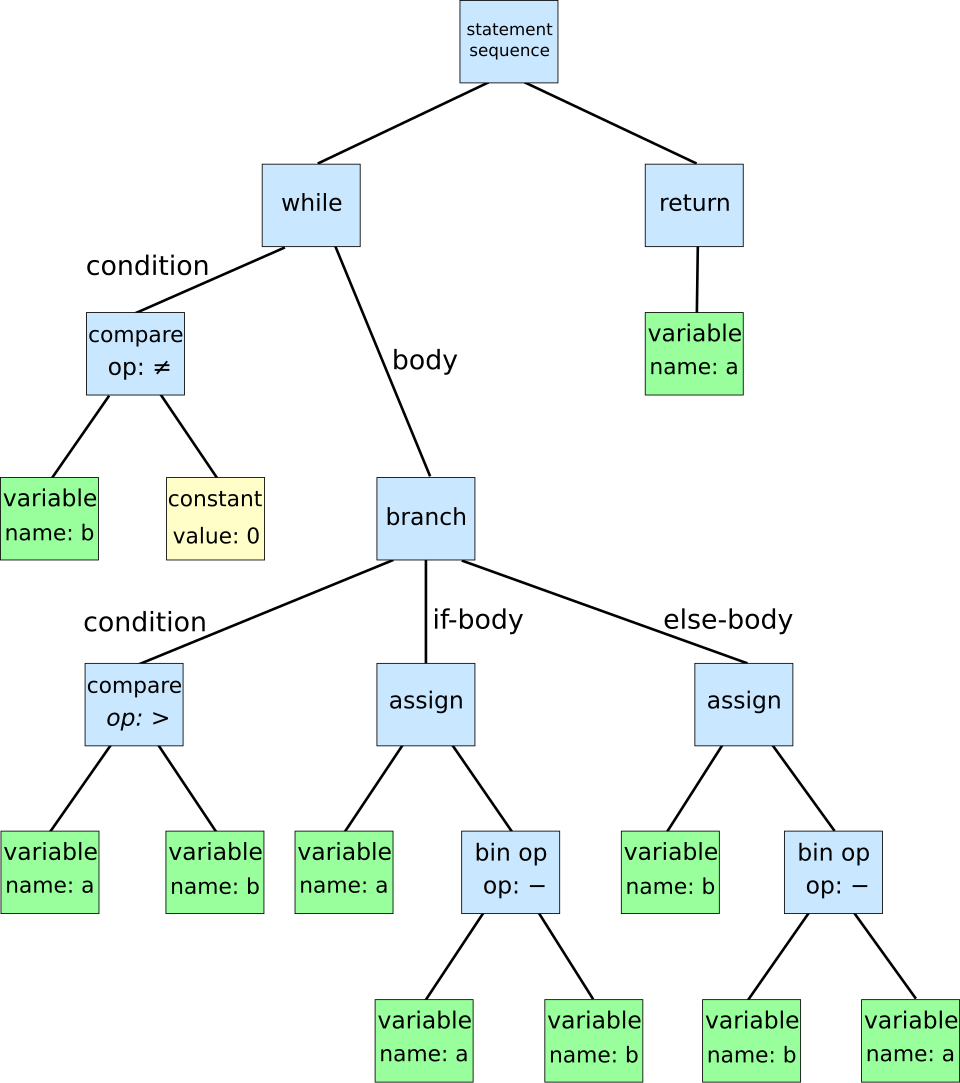
\includegraphics[width=0.95\textwidth]  {ast.svg.png}} 
	\caption{抽象语法树示例}
	\label{ast}
\end{figure}
一个常见的语法树如图\ref{ast}所示,图中的“while”,“compare”都表示实际代码中的具体控制逻辑,但是该抽象语法树并未映射任何语言。通过抽象语法树,能够高效的分析出代码的具体的控制结构。由于AST本质上是一种抽象的语法表示,不依赖于具体编程语言的语法细节。通过对不同语言的AST进行归一化处理,可以实现跨语言的结构对齐和统一建模,为多语言代码检索和迁移提供基础。由于大部分的代码结构都较为规范,因此使用AST能够很好的适配较多数的代码。并且由于AST采用树状图的结构对代码进行分析,能够便于对代码的层次关系和控制结构进行分析。基于AST可以实现对完整项目的具体拆解,是的代码搜索的颗粒度得到细化,能够有助于代码检索系统实现跨语言搜索的特性。
\subsubsection{PDG}
除了AST之外,PDG也是代码结构化表达中的重要手段。PDG能够同时刻画代码中的控制依赖和数据依赖关系,为代码的深层语义分析提供了有力工具。与AST主要关注代码的语法结构不同,PDG更侧重于描述程序执行过程中各语句之间的依赖关系。在PDG中,节点通常表示程序中的语句或操作,边则表示控制依赖,如条件分支、循环和数据依赖等。通过PDG,可以得知代码片段之间的执行顺序、变量流转和影响范围。比如,在一个if-else结构中,PDG能够明确表示条件判断对后续语句的控制影响;在变量赋值和使用的场景下,PDG能够追踪数据的流向。
\begin{figure}[H]
	\center{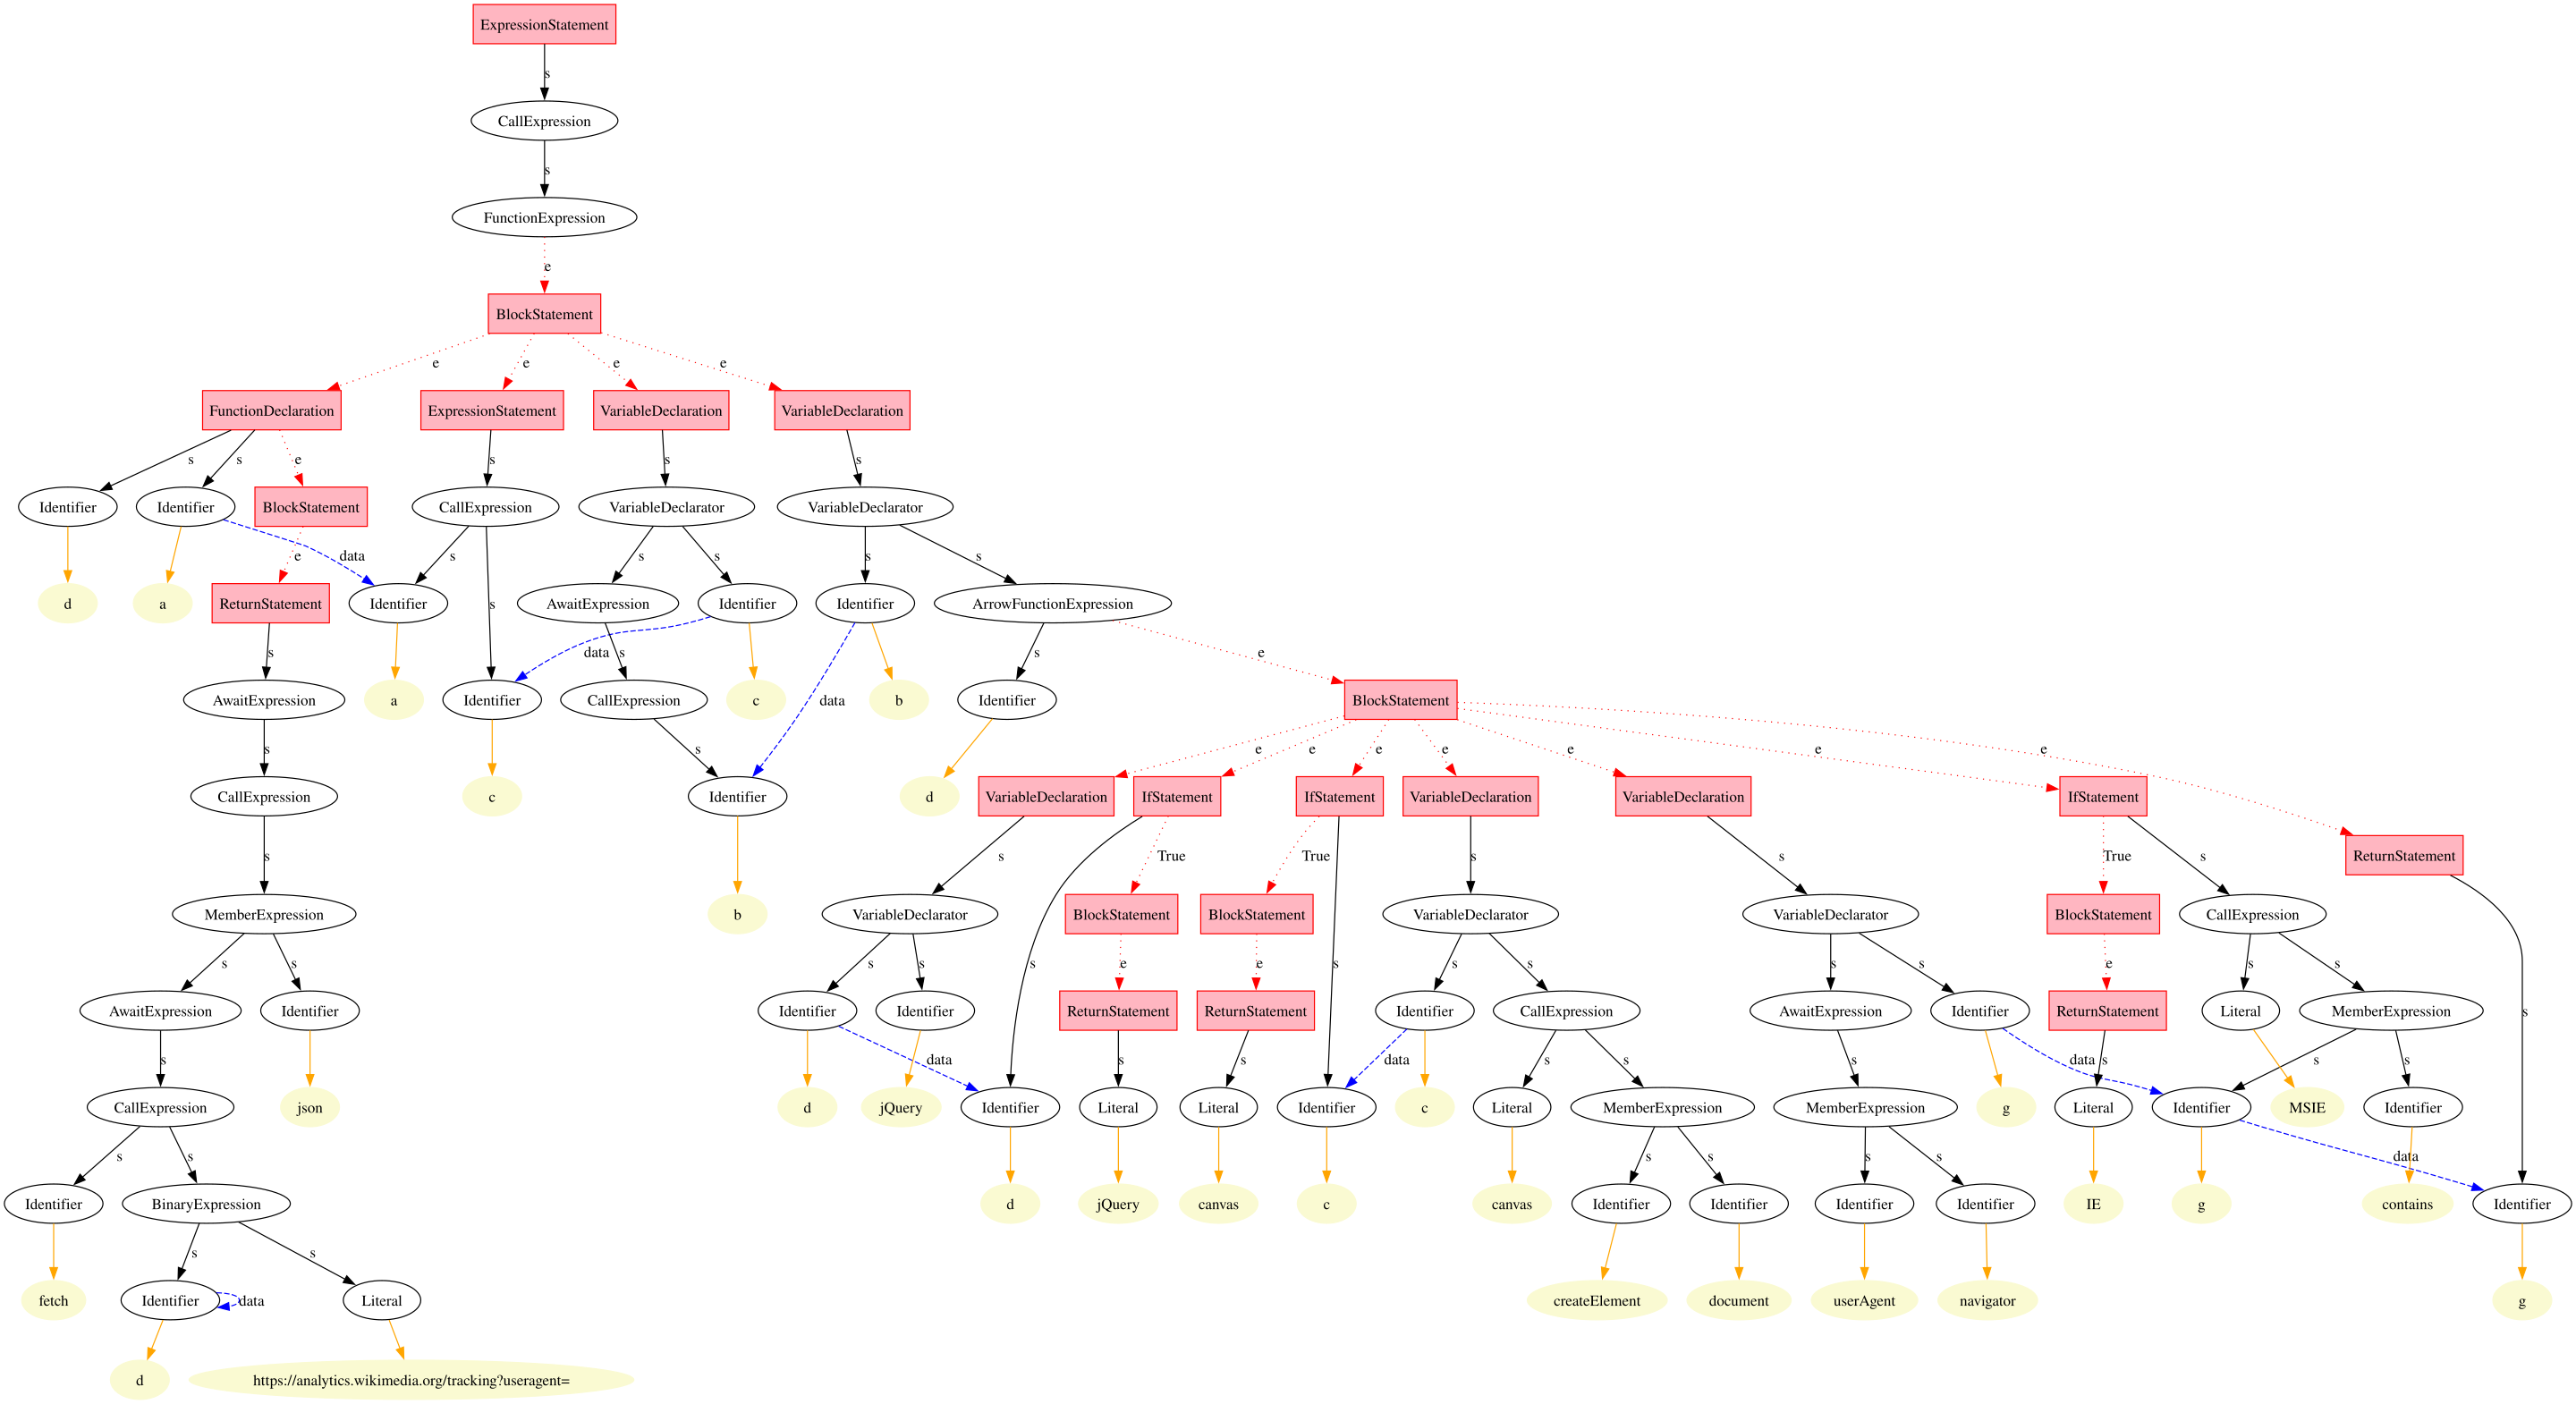
\includegraphics[width=0.95\textwidth]  {PDG.png}} 
	\caption{程序依赖图示例}
	\label{pdg}
\end{figure}
这种结构化表示对于代码克隆检测、漏洞分析、程序切片等高级软件工程任务具有重要意义。PDG的构建通常依赖于对AST和CFG的进一步分析。通过结合静态分析技术,可以自动化地从源代码中提取PDG结构。对于多编程语言的代码检索场景,PDG可以通过节点和依赖类型的归一化,实现跨语言的结构对齐和语义映射,达到跨语言检索的目的。\par
代码结构化表达方式通过将源代码从原始文本转化为统一、抽象的语法和语义表示,有效地消除了不同编程语言在表层语法上的差异,实现了代码结构和功能的归一化建模,这为构建面向多编程语言的代码检索系统提供了坚实的基础。借助代码的结构化表达,检索系统可以跨越语言壁垒,对不同语言实现的相似功能或语义进行对齐和匹配,从而支持跨语言、跨平台的高效代码搜索。

\subsection{基于分布式的高性能搜索引擎}
随着代码库规模的不断扩大和多语言,单机环境下的传统检索系统已难以满足高并发、大数据量场景下的实时性和可扩展性需求。为此,基于分布式架构的高性能搜索引擎是现代代码检索系统的核心基础设施。分布式搜索引擎通过将数据和计算任务分布到多台服务器上,显著地提升了系统的存储能力、检索吞吐量和容错性,能够满足海量代码数据的高效管理与快速检索。
\subsubsection{Apache Solr}
Apache Solr 是当前主流的开源分布式搜索引擎之一,广泛应用于大规模数据检索与分析场景。Solr 基于 Apache Lucene 构建,具备高性能、良好的可扩展性以及强大的容错能力,能够满足代码检索系统在高并发、低延迟和大数据量处理等方面的需求。Solr 采用分布式架构,通过分片(Shard)和副本(Replica)机制,将索引数据分布存储在多个节点上,实现了系统的水平扩展和高可用性。当用户发起检索请求时,Solr 会将查询任务分发到各个分片并行处理,最后将结果汇总返回,从而显著提升了检索效率和系统吞吐量。\par

\begin{figure}[H]
	\center{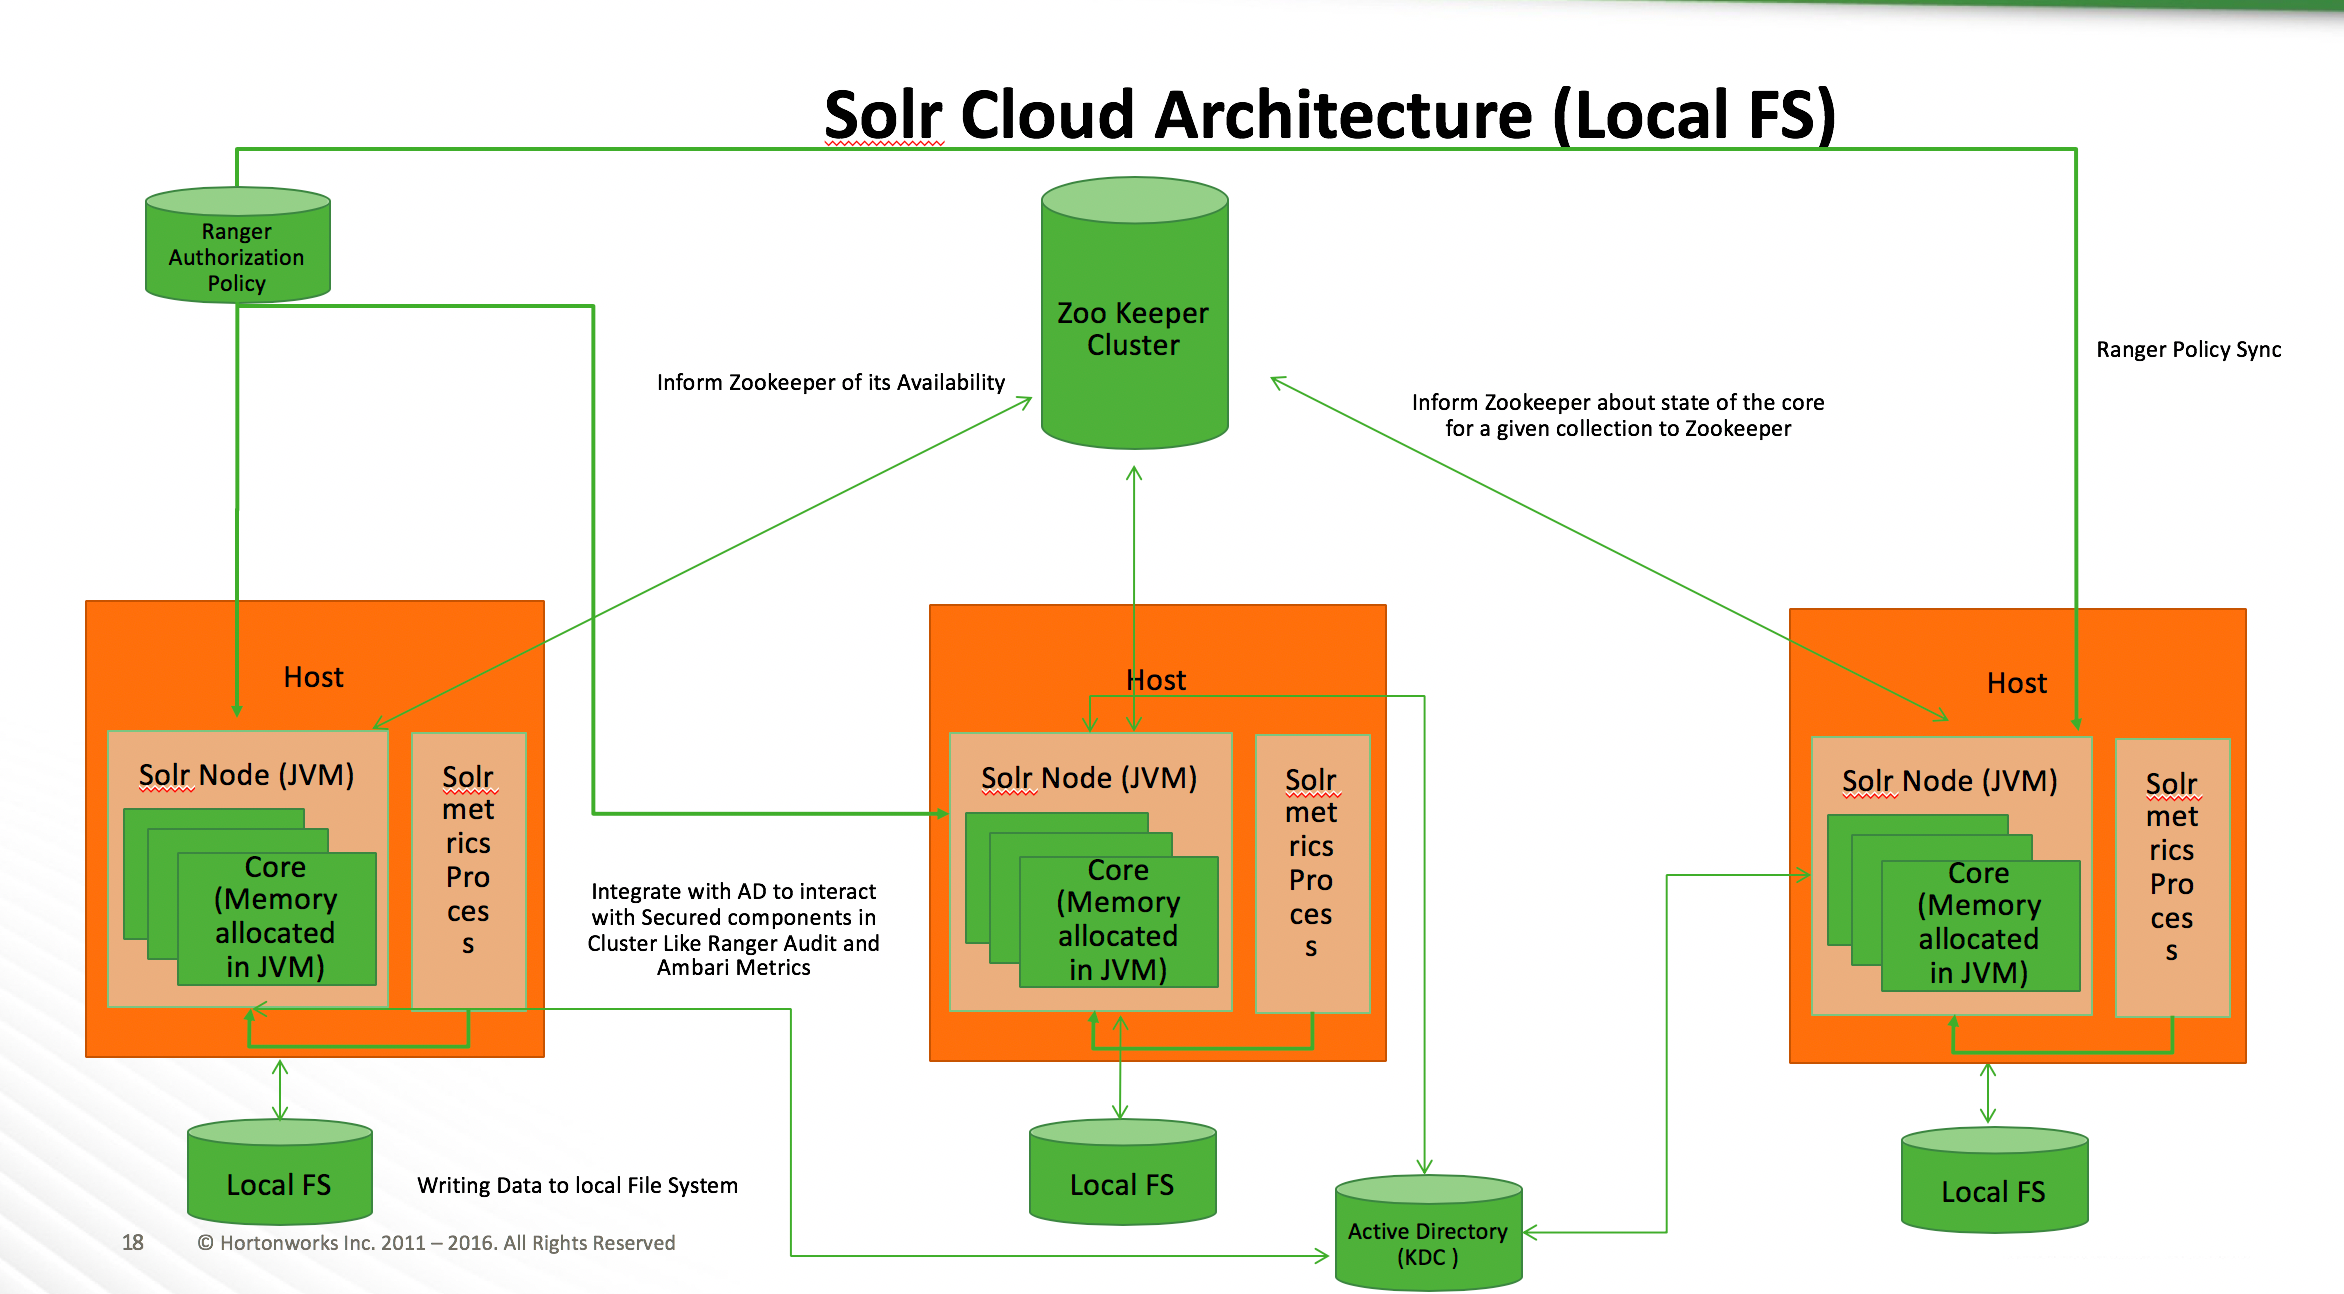
\includegraphics[width=0.95\textwidth]  {solr.png}}
	\caption{Solr结构图}
	\label{solr}
\end{figure}

如图\ref{solr}所示,Solr 的集群由一组通过 ZooKeeper 协同工作的 Solr 节点组成,并作为一个整体进行统一管理。一个集群可以包含多个集合(Collection),每个集合相当于一个独立的逻辑索引,内部包含一组文档(Document),并采用统一的配置和 Schema 进行管理。在 SolrCloud 模式下,一个集合可以被划分为多个逻辑分片(Shard),这些分片可以分布在集群中的不同节点上,实现数据的分布式存储和高可用性。而在单节点部署的 Solr 中,一个集合通常对应一个核心(Core)。核心是 Solr 的基本工作单元,代表一个独立的逻辑索引,一个节点上可以运行多个核心,实现多索引的灵活管理。\par

此外,Solr 提供了完善的 RESTful API,便于与各类应用系统集成,并支持分布式部署、负载均衡、故障转移等企业级特性,保障系统的稳定性和可扩展性。此外,Solr 支持丰富的数据类型和灵活的索引配置,能够对结构化、半结构化和非结构化数据进行高效管理。在代码检索场景中,可以将代码片段、函数、类等不同粒度的代码实体作为文档存储在 Solr 中,并结合代码结构化表达(如 AST、PDG 等)提取的特征进行索引,支持多种查询方式,包括关键词检索、布尔查询、短语匹配等。Solr 还内置了强大的全文检索、分词、排序和高亮显示等功能,便于开发者快速定位所需代码。通过这些机制,Solr 能够高效地管理和组织大规模的代码数据,全面支持分布式、高并发的代码检索需求。\par
\subsubsection{Elasticsearch}

Elasticsearch 是当前主流的开源分布式搜索与分析引擎之一,广泛应用于大规模数据的实时检索与分析场景。Elasticsearch 基于 Apache Lucene 构建,具备高性能、良好的可扩展性以及强大的容错能力,能够满足代码检索系统在高并发、低延迟和大数据量处理等方面的需求。Elasticsearch 采用分布式架构,通过分片(Shard)和副本(Replica)机制,将索引数据分布存储在多个节点上,实现了系统的水平扩展和高可用性。当用户发起检索请求时,Elasticsearch 会将查询任务分发到各个分片并行处理,最后将结果汇总返回,从而显著提升了检索效率和系统吞吐量。\par

\begin{figure}[H]
	\center{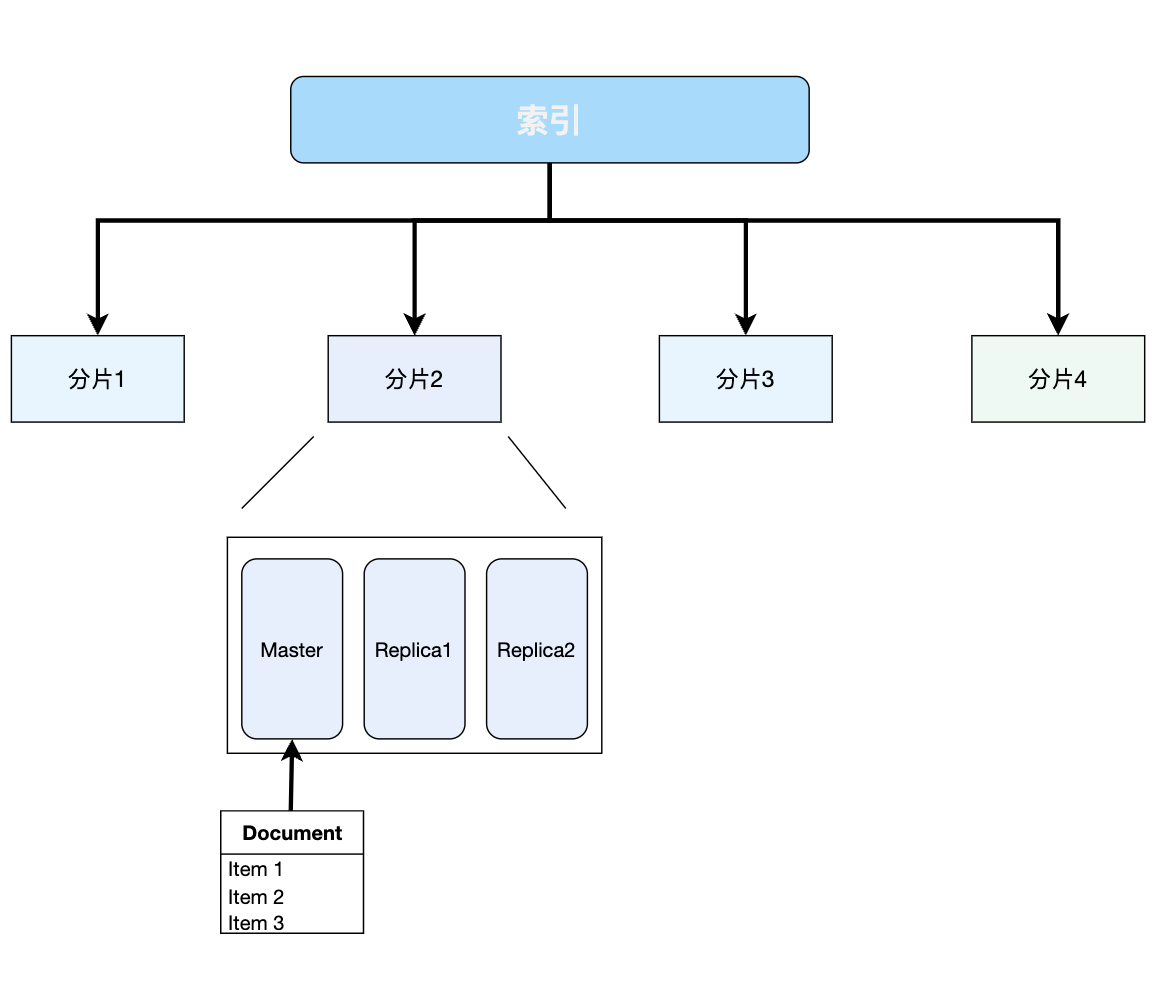
\includegraphics[width=0.95\textwidth]  {Elasticsearch.png}} 
	\caption{Elasticsearch结构}
	\label{es}
\end{figure}

如图\ref{es}所示,Elasticsearch 的集群由多个节点(Node)组成,每个节点可以承载一个或多个分片。集群中的数据以索引(Index)为单位进行组织,每个索引包含一组具有相似结构的文档(Document),并采用统一的映射(Mapping)进行管理。在多语言代码检索系统中,可以为不同的编程语言或项目类型分别建立索引,也可以将所有代码文件统一存储在一个索引中,便于统一检索和管理。需要注意的是,Elasticsearch 中的索引是逻辑上的数据集合,而分片则是物理上的数据分布单元。\par

为了实现分布式存储和提升系统的可用性与性能,Elasticsearch 引入了分片和副本的机制。每个索引可以被划分为多个主分片(Primary Shard),每个主分片又可以有一个或多个副本分片(Replica Shard)。主分片负责数据的写入和主控,副本分片则用于容错和负载均衡。当某个节点发生故障时,副本分片可以迅速接管,保证系统的高可用性和数据安全。在代码检索系统中,针对数百万个开源项目文件,可以通过合理配置分片和副本数量,优化系统的检索性能和容错能力。\par

文档(Document)是 Elasticsearch 中可被索引和检索的最小数据单元,采用 JSON 格式进行存储,类似于关系型数据库中的一行数据。在代码检索场景下,一个文档通常对应一个具体的代码文件,包含文件名、代码内容、开源协议、星数等丰富的元数据信息。通过灵活的映射配置,可以对不同类型的字段(如文本、数值、日期等)进行高效索引和检索。\par

此外,Elasticsearch 提供了功能强大的 RESTful API,便于与各类应用系统集成,并支持分布式部署、负载均衡、故障转移等企业级特性,保障系统的稳定性和可扩展性。Elasticsearch 内置了高效的全文检索、分词、聚合分析、排序和高亮显示等功能,支持多种复杂查询方式,包括关键词检索、布尔查询、短语匹配等。在代码检索系统中,可以结合代码结构化表达提取的特征进行索引,进一步提升检索的准确性和相关性。通过这些机制,Elasticsearch 能够高效地管理和组织大规模的代码数据,全面支持分布式、高并发的代码检索需求。\par
\subsection{Transformer驱动的大规模预训练语言模型}
\zihao{-4} 
大语言模型是实现本系统搜索功能的核心技术。近年来,随着代码数据规模的爆炸式增长,传统的基于关键词和规则的代码检索方法已难以满足开发者对语义理解和智能检索的需求。大语言模型凭借强大的语义建模和理解能力,能够对代码片段、函数、类等多粒度代码实体进行深层次的语义表示和推理,从而极大提升代码检索系统的智能化水平。当前,基于大语言模型的代码检索系统已成为智能开发辅助、代码推荐、自动补全等场景的关键基础设施。要深入理解当前的大语言模型,必须先了解其核心架构——Transformer。因此,本节将简要介绍Transformer及大语言模型的其他关键技术,并结合其在代码检索系统中的应用进行说明。

\subsubsection{Transformer}
Vaswani等人指出,循环神经网络模型(RNN)在每个时间步都需要依赖前一时间步的隐藏状态信息进行计算,这种固有的顺序依赖性使得RNN难以在多GPU上进行并行计算,从而限制了RNN在处理超大规模文本数据时的训练能力。为了解决这一问题,他们提出了Transformer架构,这是一种完全依赖注意力机制连接编码器和解码器的网络架构。Transformer显著提高了训练的并行度和速度。后续的一系列研究表明,基于Transformer架构的预训练模型(pre-trained models / pre-trained language models,PTM / PLM)在各种任务上都能实现最先进的性能表现,因此,Transformer已成为自然语言处理(NLP)领域的首选架构。除了在语言相关领域的应用之外,Transformer还被广泛应用于计算机视觉、音频处理以及自然科学学科,如化学、生物等领域。\par

\begin{figure}[H] 
	\center{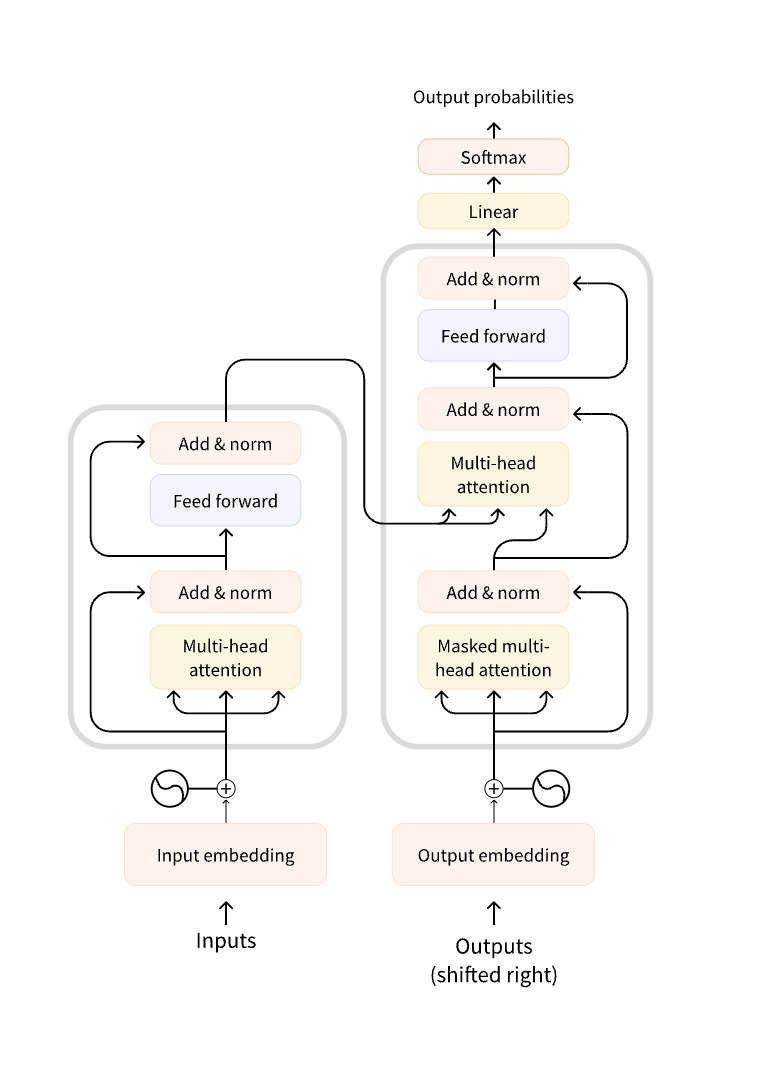
\includegraphics[width=0.95\textwidth]  {transformer.png}} 
	\caption{Transformer结构}
	\label{transformer}
\end{figure} %图表上下各空一行

Transformer架构如图\ref{transformer}所示,其整体由编码器(图\ref{transformer}左)和解码器(图\ref{transformer}右)组成。每个编码器块由多头注意力机制模块和位置前馈网络组成,模块间使用残差连接,并配有层归一化模块;解码器块在位置前馈网络和多头自注意力模块之间插入了交叉注意力模块,其中的自注意力模块用于组织某个位置信息对后续位置信息的影响。下面将简要介绍上述几种重要模块:\par
(1) 多头注意力机制:让序列中的每一个元素学习并计算与其他元素的互注意力分数权重,如公式\ref{func_1}所示:
\begin{eqnarray}
	\text{Attention(Q,K,V)} =  \text{softmax}(\frac{QK^T}{\sqrt[]{d_k}})V
	\label{func_1}
\end{eqnarray}
但Transformer并不只是简单应用了单个注意力函数,而是使用了多头注意力机制将 \(d_m\) 维度的原始 \(Q\)、\(K\)、\(V\) 分别线性投影到 \(d_k\)、\(d_k\)、\(d_v\) 维度,再根据公式\ref{func_1}进行注意力计算,整体公式如下:
\begin{eqnarray}
	\mathrm{MultiHead(Q,K,V)=~Concat(head_{1},...,head_{h})W^{O}} \\
	\mathrm{where~head_{i}~=~Attention(QW_{i}^{Q},KW_{i}^{K},VW_{i}^{V})}
	\label{func_2}
\end{eqnarray}
Transformer利用多头注意力机制能够同时关注到来自不同位置的且具有不同表示的子空间信息,增强了架构的表达能力。\par
(2) 位置前馈网络:全连接前馈网络模块,用于接收自注意力模块的输出:\par
\begin{eqnarray}
	\mathrm{FFN}(x) & =\max(0,x\mathrm{W}_1+\mathrm{b}_1)\mathrm{W}_2+\mathrm{b}_2 \\
	& =\mathrm{~ReLU(H'W}_1+\mathrm{b}_1)\mathrm{W}_2+\mathrm{b}_2
	\label{func_3}
\end{eqnarray}
(3) 残差连接与归一化:Transformer 在每个模块间使用残差连接,然后进行层归一化。其中编码器块表示为:\par
\begin{eqnarray}
	\mathrm{H^{\prime}=~LayerNorm(Self~Attention(X)+(X)} \\
	\mathrm{H=~LayerNorm(FFN(H^{\prime})+(H^{\prime})}
	\label{func_4}
\end{eqnarray}

\textbf{大语言模型与代码检索系统的关系:}  
基于Transformer的大规模预训练语言模型(如GPT、CodeBERT、Codex等)能够对自然语言查询和代码片段进行统一的语义建模,实现跨语言、跨风格的代码理解与检索。在代码检索系统中,大语言模型通常作为语义编码器,将用户的自然语言查询和代码库中的代码片段映射到同一语义空间,通过向量相似度检索相关代码。这种方法突破了传统基于关键词的检索方式,能够理解复杂的语义关系和上下文信息,显著提升了代码检索的准确率和智能化水平。此外,大语言模型还可用于代码摘要生成、代码补全、错误修复等多种智能开发场景,极大丰富了代码检索系统的功能边界。

\subsubsection{面向任务自适应的混合专家深度学习框架}
\begin{figure}[H]
	\center{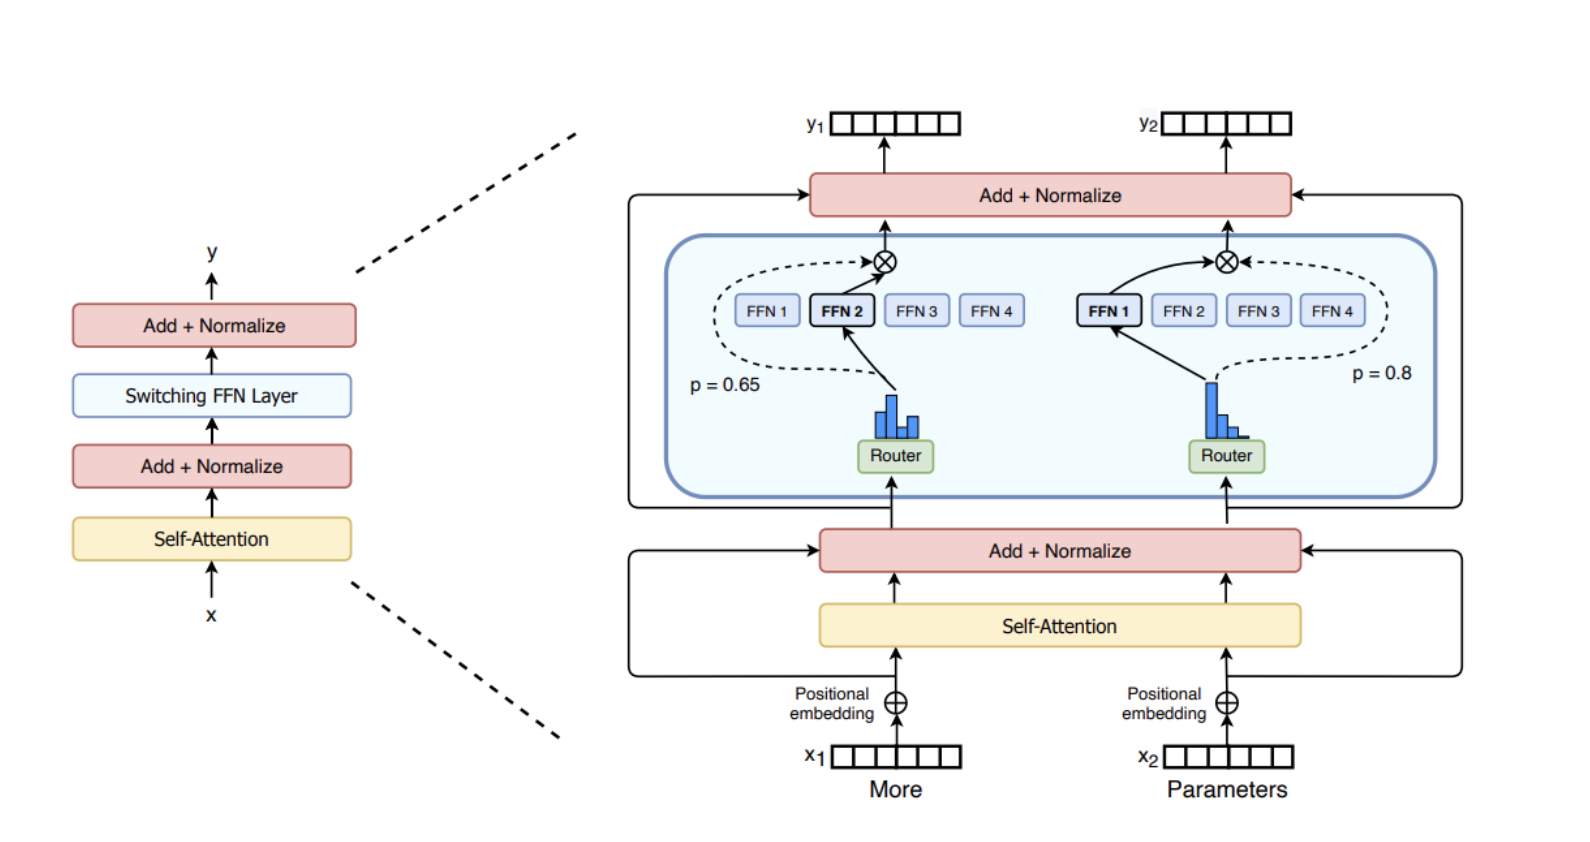
\includegraphics[width=0.95\textwidth]  {MoE.png}} 
	\caption{MoE结构}
	\label{MoE}
\end{figure}
Google Brain团队发现传统Transformer架构在扩展到超大规模时面临计算资源消耗激增的问题,尤其是前馈网络层(FFN)的全参数激活机制导致训练和推理效率急剧下降。为此,他们提出基于混合专家模型(Mixture of Experts, MoE)的稀疏架构改造方案,通过将Transformer中的FFN层替换为动态路由的专家网络集合,实现计算效率与模型容量的平衡。MoE架构如图\ref{MoE}所示,其核心创新在于引入稀疏门控机制(图\ref{MoE}蓝色部分),该机制由可学习的路由网络构成,针对每个输入词元生成专家选择概率分布,仅激活概率最高的前K个专家(通常K=2-4),其余专家保持非激活状态。具体而言,每个MoE层包含N个独立的前馈网络作为专家(例如N=8或32),其数学表达为:
\begin{eqnarray}
	\mathrm{MoE}(x)=\sum_{i=1}^KG(x)_i\cdot E_i(x)
	\label{func_5}
\end{eqnarray}
其中$G(x)$为门控网络输出的Top-K权重,$E_i(x)$为被选中的专家网络输出。这种设计使得模型总参数量可扩展至万亿级别,而实际计算量仅与激活专家数相关。实验表明,Switch Transformer在同等计算资源下,训练速度较传统稠密模型提升4倍,且推理时内存占用降低至1/4。进一步地,通过引入噪声注入(Noisy Top-K Gating)和负载均衡损失函数,MoE有效缓解了专家利用率不均衡问题,例如GLaM模型以1.2万亿参数仅激活97亿参数即达到GPT-3的97\%性能。当前,MoE架构已在GPT-4、DeepSeek、Mixtral 8x7B等主流大模型中广泛应用,成为突破单一模型规模瓶颈的核心技术路径。

\subsubsection{基于语义增强的大模型提示工程}
提示(Prompt)是一系列提供给大语言模型的指令,我们可以通过自定义提示来增强、改善大语言模型的能力。Reynolds等人首次系统性地提出Prompt作为调控大型语言模型行为的核心接口,其本质是通过自然语言指令或结构化模板显式定义输入规范、处理规则及输出约束,从而动态重构大语言模型的上下文推理路径以适配特定任务需求。比如,可以指定大语言模型在生成文档时标记重点内容;可以指定大语言模型只输出符合要求的关键词语;可以指定大语言模型只生成指定代码风格的代码等。\par

提示工程(Prompt Engineering)作为一种独特的编程模式,主要围绕向大型语言模型精准输入提示展开操作。本质上,这一过程需要精心设计适配的提示模板,以此助力完成特定的下游任务。实践表明,优化提示内容能够显著提升模型在各类任务中的表现。\par

\begin{figure}[H]
	\center{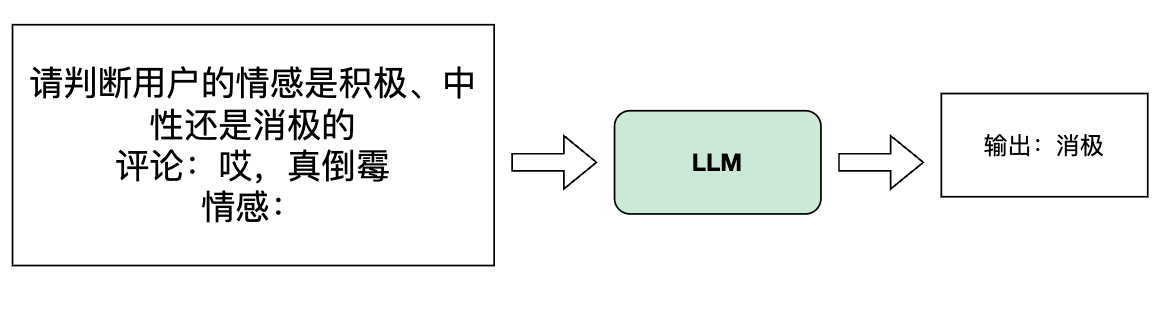
\includegraphics[width=0.95\textwidth]  {zero_shot.png}}
	\caption{零样本提示示例}
	\label{zero_shot}
\end{figure}
\begin{figure}[H]
	\center{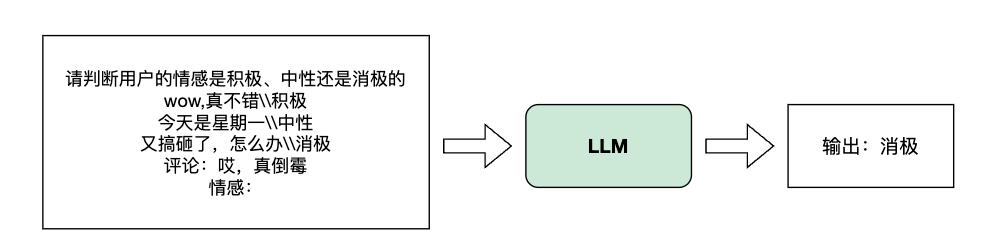
\includegraphics[width=0.95\textwidth]  {few_shot.png}}
	\caption{少样本提示示例}
	\label{few_shot}
\end{figure}
在提示工程的实际应用中,零样本提示(Zero-Shot Prompting)是一种基础方法,图\ref{zero_shot}展示了相关示例。该方法下,即便不向模型提供任何参考示例,模型也能够给出有价值的回应,完成既定任务。然而,当零样本提示无法满足需求时,少样本提示(Few-Shot Prompting)便派上用场,如图\ref{few_shot}。此时,需针对下游任务设计专门的提示模板,模板不仅要囊括一系列大语言模型处理规则,还要为后续待输入文本预留特定位置。在向大语言模型发起询问时,只需将待输入文本填充至提示模板预留空位,即可构建完整提示。除此之外,开启思维链、给大语言模型指定角色性格等提示技巧都能显著改变大语言模型输出效果和对任务的执行情况。\par
进一步看,巧妙构建提示能够催生全新的交互模式。借助提示指令,大语言模型可生成与软件工程概念相关的测验题目,模拟程序运行流程,甚至模拟命令行终端窗口的交互场景。不仅如此,提示还具备自适应特性,部分提示能够依据当前情况,推荐其他提示,以便收集更多信息,或生成相关成果物。提示的这些进阶功能,充分彰显了深入设计提示、挖掘其在简单文本与代码生成之外价值的重要意义。\par
在代码检索系统中,提示工程不仅可以用于优化自然语言查询的表达方式,还能引导大语言模型更好地理解用户意图,实现更为精准的代码匹配。通过设计针对代码风格、功能描述、编程语言等维度的提示,可以让大语言模型在检索和生成代码时更加贴合实际开发需求。此外,提示工程还可用于多轮对话、代码解释、错误定位等场景,提升代码检索系统的人机交互体验和智能化水平。
\subsection{基于微服务的高可用后台架构}
\zihao{-4}
微服务架构是本系统实现的核心技术之一,与微服务相对应的是传统的单体架构方案。单体架构(如图\ref{compare}左所示)将整个系统封装在一个程序中,集成了登录、鉴权、业务逻辑、数据处理等所有功能模块。这种“大而全”的架构对于小型系统而言,能够缩短开发周期,且开发和部署流程相对简单,符合开发者的直觉和习惯。然而,随着系统规模的扩大和业务复杂度的提升,单体架构逐渐暴露出模块耦合度高、扩展性差、维护成本高等问题,难以满足高并发、大数据量和多语言支持等现代应用场景的需求。\par
相比之下,微服务架构采用了“高内聚、低耦合”的设计理念,将系统的各个功能模块拆分为独立的服务,每个服务专注于完成某一特定功能,并以单独的进程或容器形式运行。整个系统由一组相互协作的微服务构成,服务之间通过网络进行通信(如图\ref{compare}右所示)。微服务架构的核心特点在于服务的颗粒度更细,职责更加单一,便于独立开发、测试、部署和扩展。通常情况下,每个微服务会运行在 Docker 容器中,而 Kubernetes 则负责对这些服务进行高效的管理和编排。通过这种方式,微服务架构不仅提升了系统的灵活性和可扩展性,还为大型复杂系统的开发和维护提供了更强的支持。\par

\begin{figure}[H]
	\center{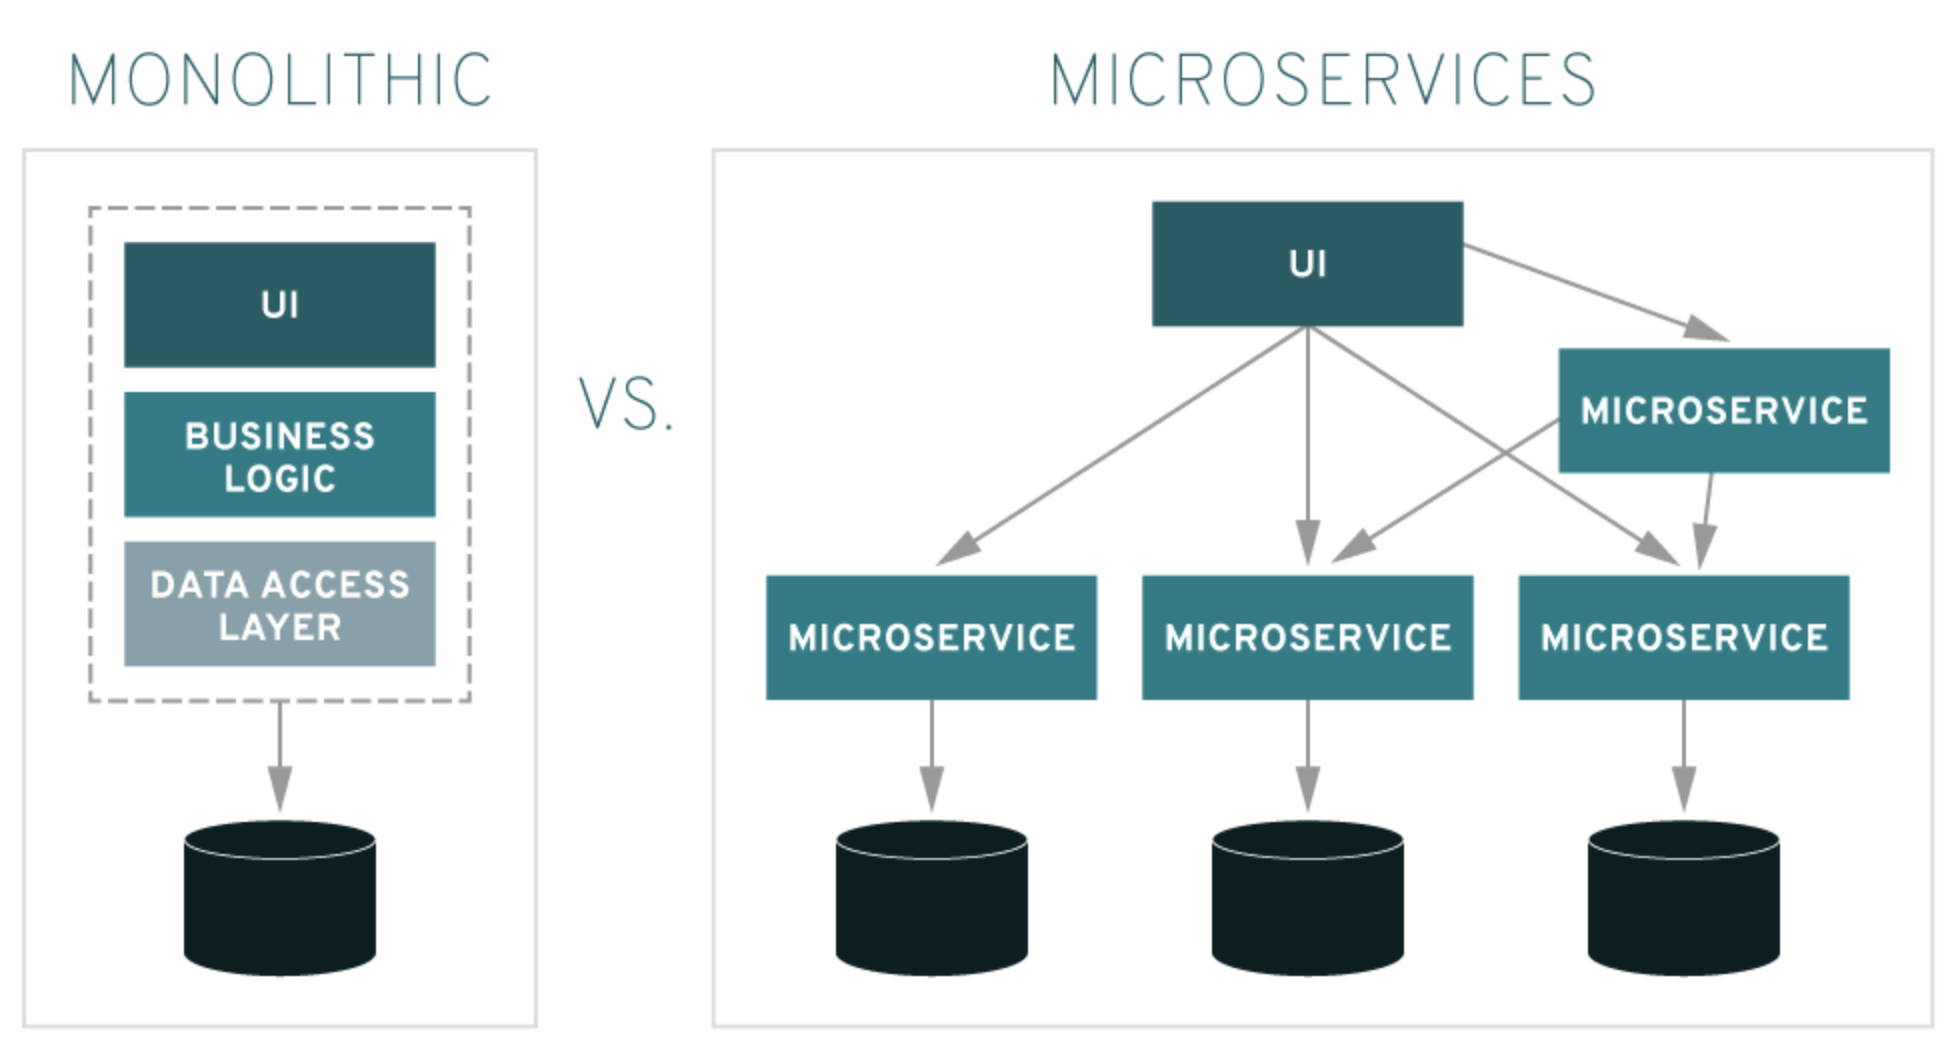
\includegraphics[width=0.95\textwidth]  {compare.png}} 
	\caption{单体架构和微服务架构对比}
	\label{compare}
\end{figure}
对于构建面向多编程语言的代码检索系统而言,系统通常需要处理多种编程语言的解析、索引、检索、语义分析等复杂任务,同时还需要依赖大模型实现检索词的检索增强功能。不同编程语言的处理逻辑、依赖环境和扩展需求各不相同,单体架构难以灵活应对多语言场景下的异构需求。但是对于微服务而言,每个微服务可以采用最适合其功能的编程语言和技术栈。例如可以使用Python服务部署大语言模型,实现系统中的检索增强功能,使用Go语言搭建的网关、鉴权、检索等服务可以应对高并发的请求处理,以及业务的安全校验。这样不仅提升了开发效率,也方便集成社区已有的多语言处理工具。同时针对不同模块的微服务而言,可以独立扩展相关微服务的实例数,实现资源的动态分配和弹性伸缩。比如对于网关这类的服务而言,往往是IO密集型而非CPU密集型,因此在部署的时候可以考虑使用轻量级的容器实例进行横向扩展,以应对高并发的网络请求压力;而对于大语言模型推理服务,则通常是计算密集型任务,可以部署在具备GPU加速能力的节点上,并根据实际负载动态调整模型服务的副本数,从而实现资源的高效利用和系统整体的弹性伸缩。此外,微服务架构还支持服务的独立升级与灰度发布。当需要对某一编程语言的解析模块进行功能优化或安全加固时,只需对对应的微服务进行迭代和部署,无需影响其他服务的正常运行。这种解耦的架构极大降低了系统维护和演进的复杂度,提升了系统的可维护性和可用性。在多语言代码检索系统中,微服务架构还便于集成和管理多种第三方工具与智能组件。例如,可以为不同编程语言分别集成专用的语法分析器、静态检查工具或代码格式化服务,也可以灵活接入多种大语言模型用于语义增强、代码补全或自然语言查询理解。各服务之间通过gRPC等高效协议进行通信,保证了系统的高性能和低延迟。\par
因此,微服务架构为面向多编程语言的代码检索系统提供了高可用、高扩展性和高灵活性的基础设施保障,是支撑大规模、智能化代码检索服务的关键技术路径。\par

\subsubsection{跨语言的远程调用框架}
gRPC是一种高性能、开源的跨语言远程过程调用(RPC)框架,广泛应用于微服务架构下的服务间通信。gRPC允许客户端应用程序直接调用服务器端应用的方法,就像它们是本地对象一样,这使得分布式应用程序开发变得更加容易。gRPC使用HTTP/2作为传输协议,支持双向流、头部压缩等特性,从而提供了更高效的网络通信。此外,gRPC通过Protocol Buffers定义接口和服务,这是一种轻量级、跨平台的消息格式,有助于提高数据交换效率并减少带宽使用。在微服务架构中,gRPC因其高效性而被广泛用于服务间通信。\par
在gRPC中,服务定义和数据交换格式通常使用Protocol Buffers。Protocol Buffers是由Google设计的一种轻量级、跨平台的消息格式,用于序列化结构化数据。通过.proto文件,开发者可以定义自己的数据结构和服务接口。这些定义被编译成不同编程语言的代码,以便生成易于使用的类来构建强类型的请求和响应消息。与其他序列化协议(如JSON、XML、BSON等)相比,protobuf采用二进制编码,消息体积小,传输高效,适合高并发和大数据量场景。除此之外,protobuf支持多种编程语言,gRPC自带的编译工具可快速生成多语言桩代码,适合多语言协作的微服务架构。并且protobuf通过为字段分配唯一标识符,支持消息格式的平滑演进,保障了系统的长期可维护性。

\subsubsection{容器化部署与环境隔离基础设施}
Docker是一个开源的应用容器引擎,使开发者可以将应用程序及其依赖打包到一个可移植的容器中,然后发布到任何流行的Linux或Windows机器上,也可以实现虚拟化。容器采用沙箱机制,彼此隔离,安全性高。Docker容器的轻量化和快速部署能力使其成为微服务架构中的理想选择。每一个微服务都可以被打包成一个独立的Docker容器,确保了环境一致性,简化了开发、测试和部署流程。同时,由于Docker容器的资源消耗低,多个容器可以在同一台物理机上高效共存,提高了资源利用率。Docker采用联合文件系统(Union File System)技术,将不同的文件系统层叠加在一起,形成统一视图。每个Docker镜像由一系列只读层组成,创建容器时会在最顶层添加一个可写层。层次化设计不仅加快了镜像构建和分发过程,还提升了数据隔离性和安全性(如图\ref{docker})。\par
\begin{figure}[H]
	\center{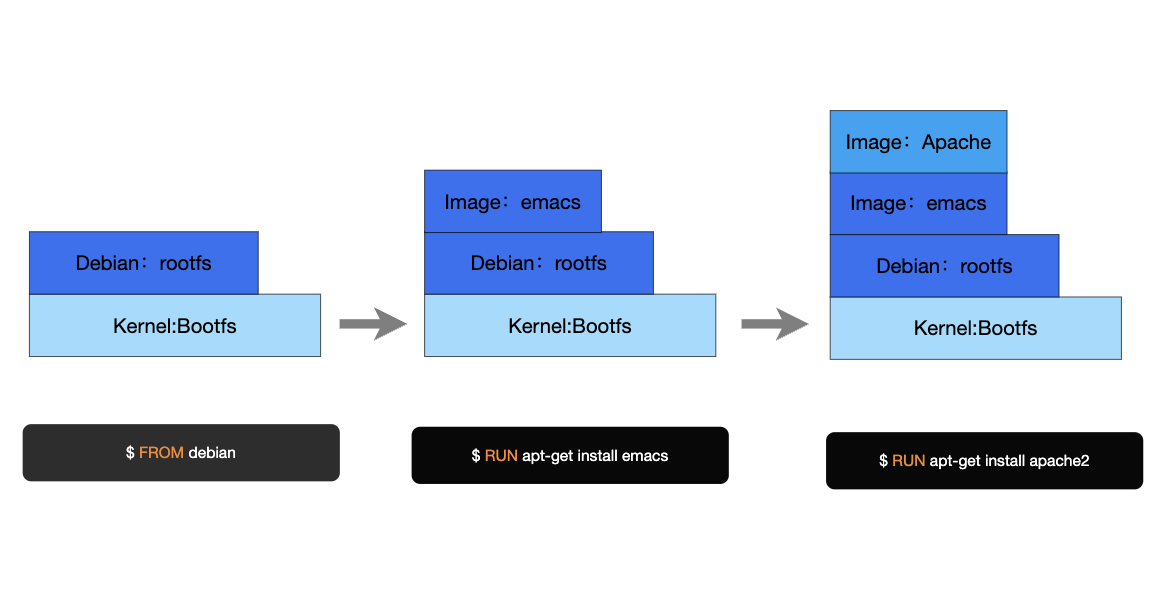
\includegraphics[width=0.95\textwidth]  {docker.png}} 
	\caption{docker层次化构建示例}
	\label{docker}
\end{figure}

\subsubsection{自动化编排与弹性伸缩的云原生平台}
\begin{figure}[H]
	\center{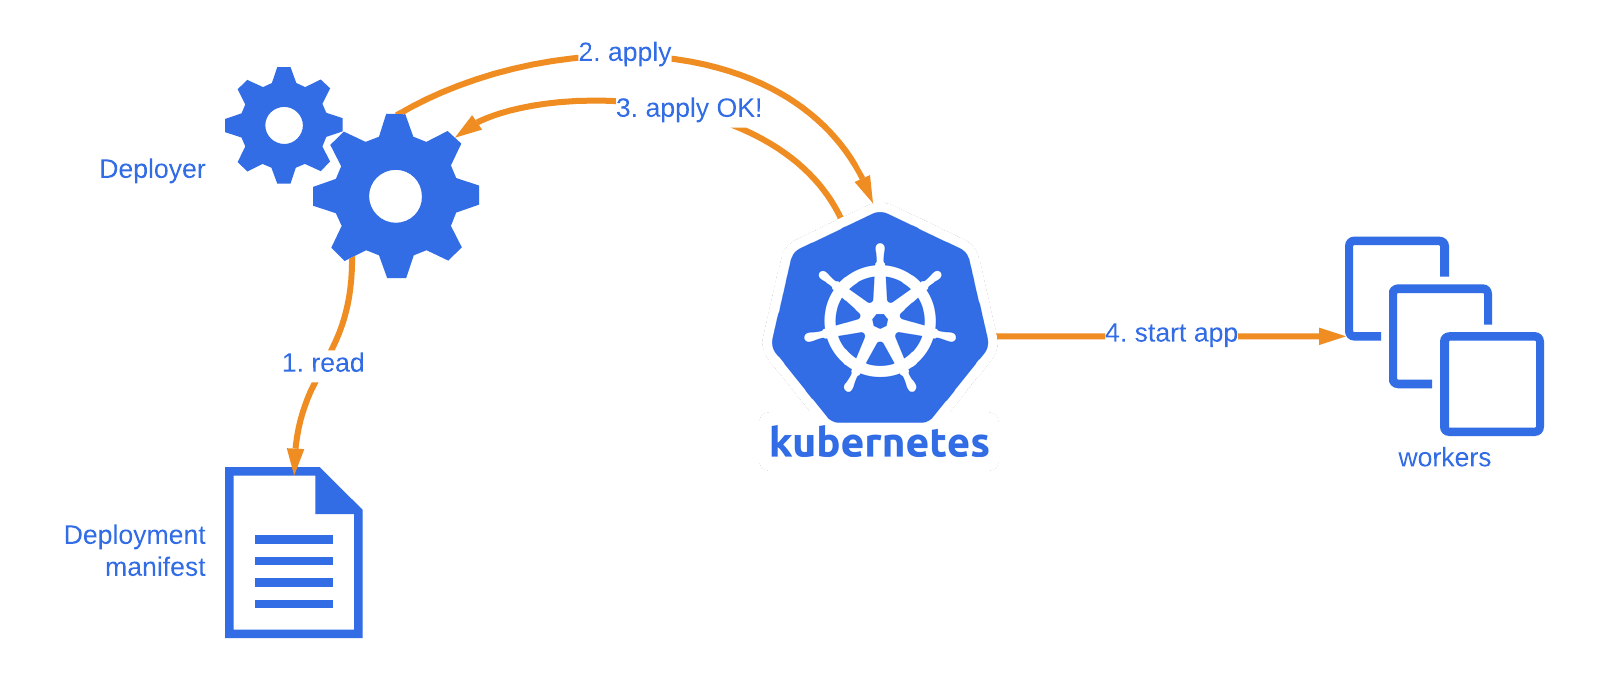
\includegraphics[width=0.95\textwidth]  {k8s_m.png}} 
	\caption{Kubernetes交互过程}
	\label{k8s_m}
\end{figure}
Kubernetes是一个用于自动化部署、扩展和管理容器化应用程序的开源平台。如图\ref{k8s_m}所示,用户可以通过简单地配置Kubernetes的编排文件就能实现对整个系统的集中资源调度。它最初由Google设计,现在由Cloud Native Computing Foundation (CNCF)维护。Kubernetes提供了一个强大的框架来运行分布式系统,能够处理负载均衡、故障转移、自我修复以及水平扩展等任务。Kubernetes 的架构如图\ref{k8s_structure}所示,主要由一个 Master 节点和多个工作节点(Node)组成。Master 节点中的 kube-apiserver 作为系统的网关,负责所有指令的转发;kube-scheduler 负责资源调度,将任务分配到合适的节点;controller 负责维护系统中所有资源对象的状态;etcd 用于存储所有资源对象的数据。在 Node 节点上,kubelet 负责执行资源操作指令,kube-proxy 实现服务间的负载均衡,Pod 作为 Kubernetes 管理的最小单元,内部运行一个或多个容器,容器引擎(如 Docker)则为容器提供运行环境。在微服务架构中,Kubernetes 负责管理和编排各个微服务的生命周期与交互,确保所有服务能够高效、稳定地协同工作。通过自动化的滚动更新和回滚机制,Kubernetes 极大地简化了应用的维护流程,降低了人为操作失误的风险。\par
\begin{figure}[H]
	\center{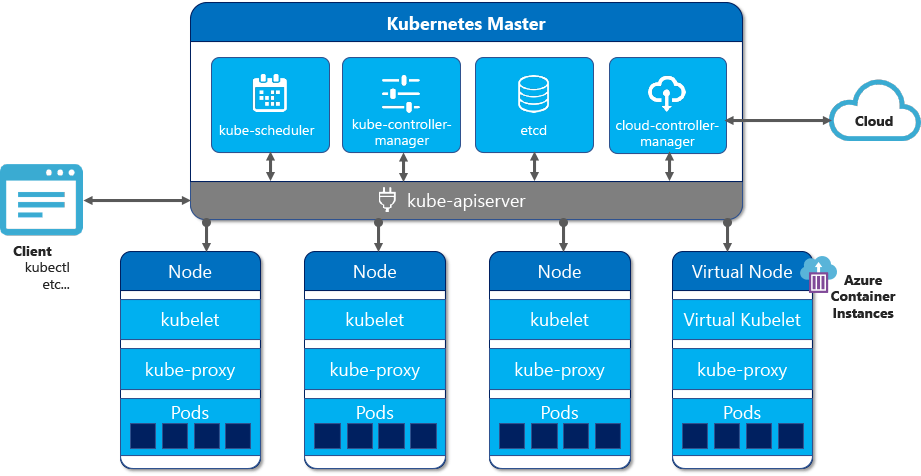
\includegraphics[width=0.95\textwidth]  {k8s_structure.png}} 
	\caption{Kubernetes结构}
	\label{k8s_structure}
\end{figure}
综上,微服务架构通过解耦系统功能、支持多语言开发、提升可扩展性和高可用性,为面向多编程语言的代码检索系统提供了坚实的技术基础。结合gRPC、Docker和Kubernetes等现代云原生技术,高效地支撑了大规模、异构、智能化的代码检索服务,满足了复杂业务场景下的高并发、低延迟和持续演进的需求。
\subsection{面向高效开发的VS Code插件生态与创新实践}
\zihao{-4}
为了高效构建美观且用户友好的交互界面,VS Code通过支持TypeScript或JavaScript实现其官方接口,显著简化了开发流程。此外,VS Code允许在侧边栏(Side Bar)中嵌入WebView页面,这一特性为开发者提供了利用前端框架开发插件的可行性,极大降低了技术学习门槛。在持续开发与维护前端项目时,选择成熟框架已成为关键策略。Vue.js作为主流前端框架,已迭代至Vue 3版本。其庞大的开源生态(如Element Plus等UI组件库)为开发者提供了丰富的可视化资源,即使缺乏专业设计支持,也能快速构建出美观的界面。相较于前代版本,Vue 3在响应式系统、组件化开发及性能优化等方面引入了多项革新性改进。本章节将系统性地介绍Vue.js框架的核心特性,\par
\subsubsection{基于组件化思想的Vue框架}
Vue.js是一套渐进式JavaScript框架,凭借其轻量级架构、低学习门槛、高效性能等核心优势,已成为全球范围内最受欢迎的前端框架之一。作为渐进式框架的典型代表,Vue.js的设计以灵活性为核心原则,开发者可根据实际需求逐步采用其提供的功能模块,而非强制要求一次性全面使用所有特性。这种渐进式特性使其既能满足小型项目的快速开发需求,又能支撑大型应用的复杂架构。\par
在设计模式方面,Vue采用模型-视图-视图模型(Model-View-ViewModel,MVVM)架构(图\ref{MVVM}所示)。相较于传统的MVC模式,Vue的MVVM模式实现了视图与模型的解耦,并通过视图模型(ViewModel)层实现数据的无缝双向绑定。该模式通过数据绑定和视图自动更新机制,显著减少了冗余代码的编写,使开发者能够将精力集中于核心业务逻辑与界面设计的优化。\par
\begin{figure}[H]
	\center{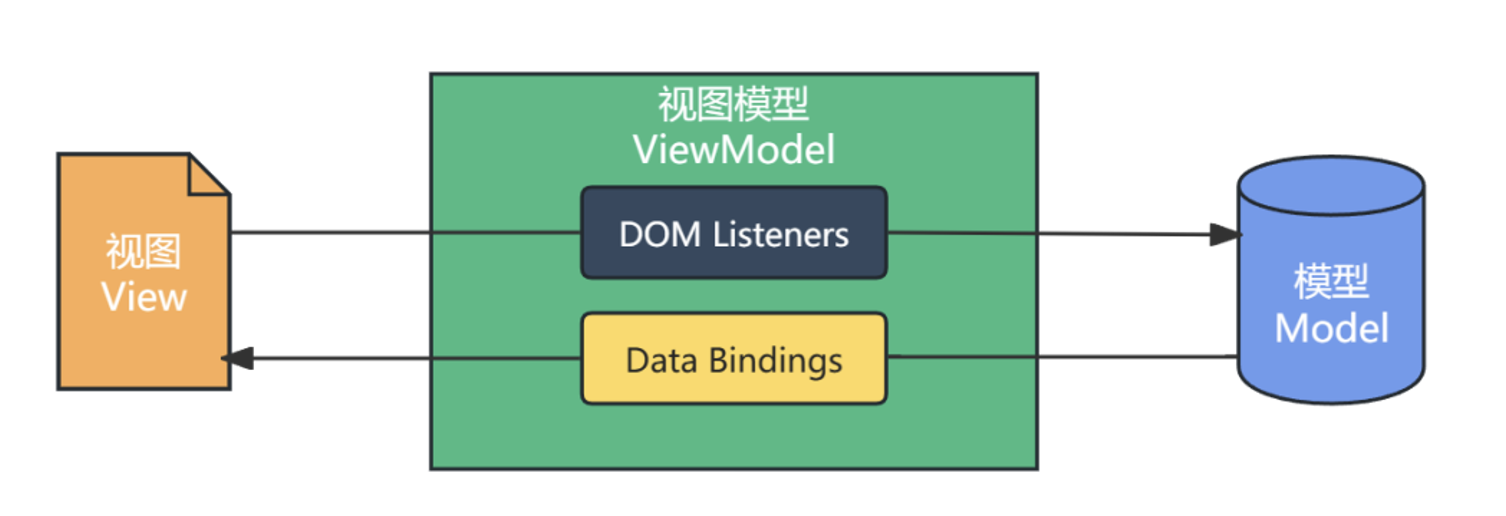
\includegraphics[width=0.95\textwidth]  {MVVM.png}} 
	\caption{Vue的MVVM设计模式}
	\label{MVVM}
\end{figure}
在技术特性方面,Vue.js引入了虚拟DOM(Virtual DOM)与响应式数据系统。其中,响应式系统通过实时追踪状态变化,能在数据更新时智能驱动视图的局部渲染,从而大幅减少直接操作DOM的频率。这一机制不仅降低了开发复杂度,更避免了频繁调用DOM对象的性能损耗,使开发者得以专注于业务逻辑的实现。\par
\subsection{本章小结}
\zihao{-4} 
本章介绍了实现面向多编程语言的代码检索系统的核心理论和技术。首先介绍了代码检索问题的基本内涵及其在现代软件工程中的重要意义,分析了代码结构化表达(如AST、PDG等)对于实现跨语言、深层次代码理解与检索的基础作用。随后,详细阐述了分布式高性能搜索引擎(如Solr、Elasticsearch)在大规模代码数据管理与高并发检索中的应用优势,为系统的可扩展性和高可用性提供了有力支撑。在智能检索层面,重点解析了以Transformer为代表的大规模预训练语言模型的原理及其在代码语义建模、跨语言检索等场景中的应用价值。进一步介绍了混合专家模型(MoE)等前沿深度学习架构在提升模型容量与推理效率方面的创新,以及基于提示工程的语义增强方法对大语言模型能力的优化和扩展。通过这些技术,系统能够实现对自然语言查询和多语言代码的统一语义理解,显著提升检索的准确性和智能化水平。在系统架构方面,论述了微服务架构在多语言代码检索系统中的关键作用。微服务通过服务解耦、异构技术栈支持、弹性伸缩和高可用性,极大提升了系统的灵活性和可维护性。结合gRPC、Docker和Kubernetes等云原生技术,实现了高效的服务通信、环境一致性和自动化运维,满足了大规模、复杂业务场景下的高并发和持续演进需求。最后,介绍了面向高效开发的VS Code插件生态,重点分析了Vue.js等现代前端框架在提升用户交互体验和开发效率方面的优势。通过插件化和组件化开发模式,系统能够为开发者提供美观、易用的代码检索界面,进一步增强了系统的实用性和用户粘性。
\newpage
\fancyhead[LH]{\zihao{-5}{\songti 重庆大学本科学生毕业论文(设计)}}
\fancyhead[RH]{\zihao{-5}{\songti 3\quad 系统需求分析与设计}}
\section{面向多编程语言的代码检索系统需求分析}
随着多语言协同开发模式的日益普及,开发者在实际软件工程实践中面临着跨语言代码检索与复用的复杂需求。传统的代码检索系统已难以满足当前多样化、智能化的开发场景。为此,本文致力于设计并实现一套面向多编程语言的高效代码检索系统。本章将在前述研究背景与相关理论技术的基础上,系统分析该系统的功能需求与技术挑战,提出整体架构设计方案,并详细阐述各核心模块的设计思路与关键技术实现。本章将主要围绕面向多编程语言的代码检索系统的需求分析与设计实现展开,内容包括系统需求分析、系统架构设计、业务功能设计等。首先,从用户需求及系统的功能性与非功能性需求出发,对系统进行全面深入的需求分析。随后,依据需求分析结果,对系统进行详细解析,设计总体架构以及前后端服务架构。最后,重点围绕项目存储、大模型提示词工程等关键功能模块,展开系统的业务功能设计,为系统的高效实现奠定基础。
\subsubsection{用户需求}
本系统的核心目标是为开发人员提供高效便捷的代码检索支持,通过智能化的自然语言搜索能力辅助开发流程,显著提升代码复用效率与开发质量。整体用户需求示意图如图\ref{flow}所示。对于系统用户,可以在VS Code平台插件商城中下载该系统的插件,通过系统的身份认证后即可在开发环境中的侧边栏打开使用该系统,或者使用内置的快捷键也能实现多编程语言搜索的功能。对于系统的运维人员,可以根据本项目的开源平台的项目README指引部署系统,并且通过手动新增或者删除项目的方式管理系统的搜索范围。
\begin{figure}[H]
	\center{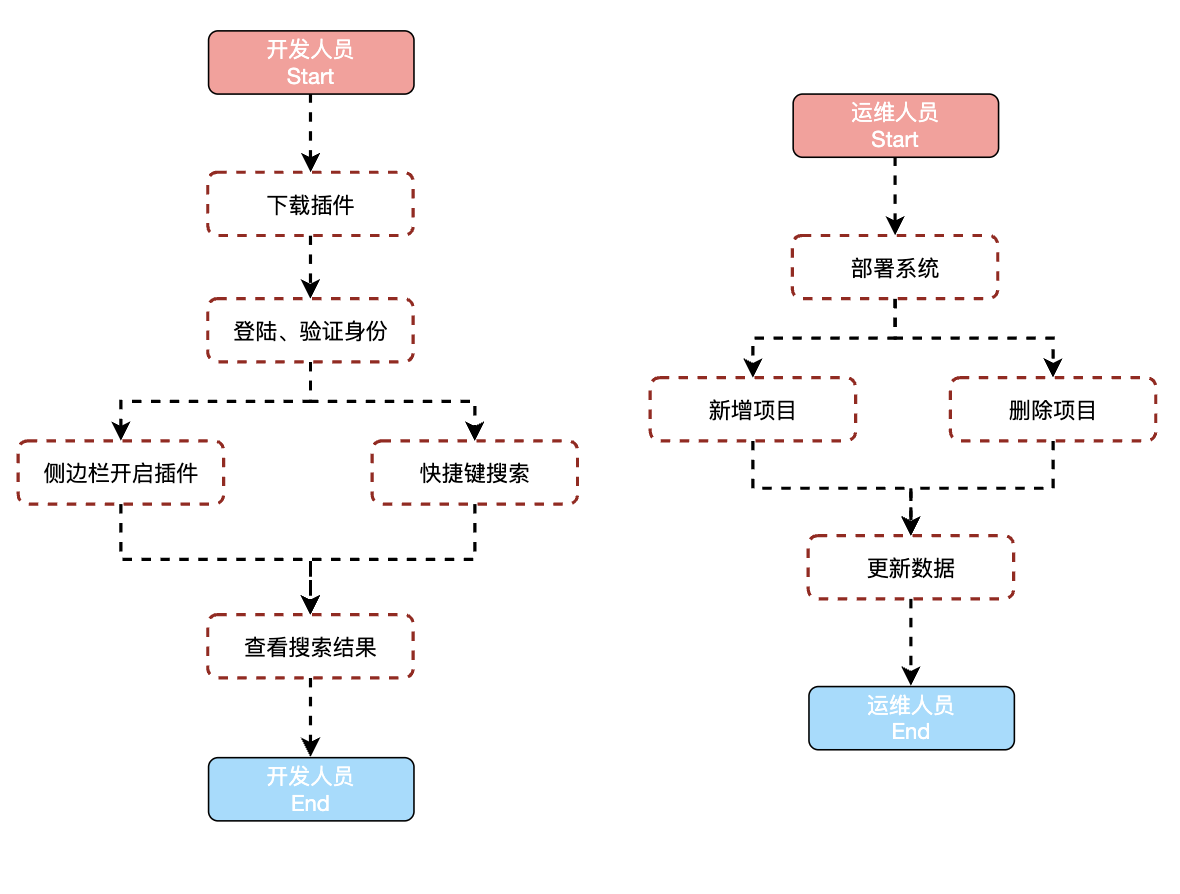
\includegraphics[width=0.95\textwidth]  {flow.png}} 
	\caption{整体用户需求示意图用例图}
	\label{flow}
\end{figure}
\subsubsection{系统功能性需求分析}
本节将根据用户需求,明确系统核心功能性需求,本小节根据系统不同角色定位,做如下功能性需求分析:\par
对于开发者用户,做如下功能分析,图\ref{user}为开发人员的功能需求用例图:\par
\begin{figure}[H]
	\center{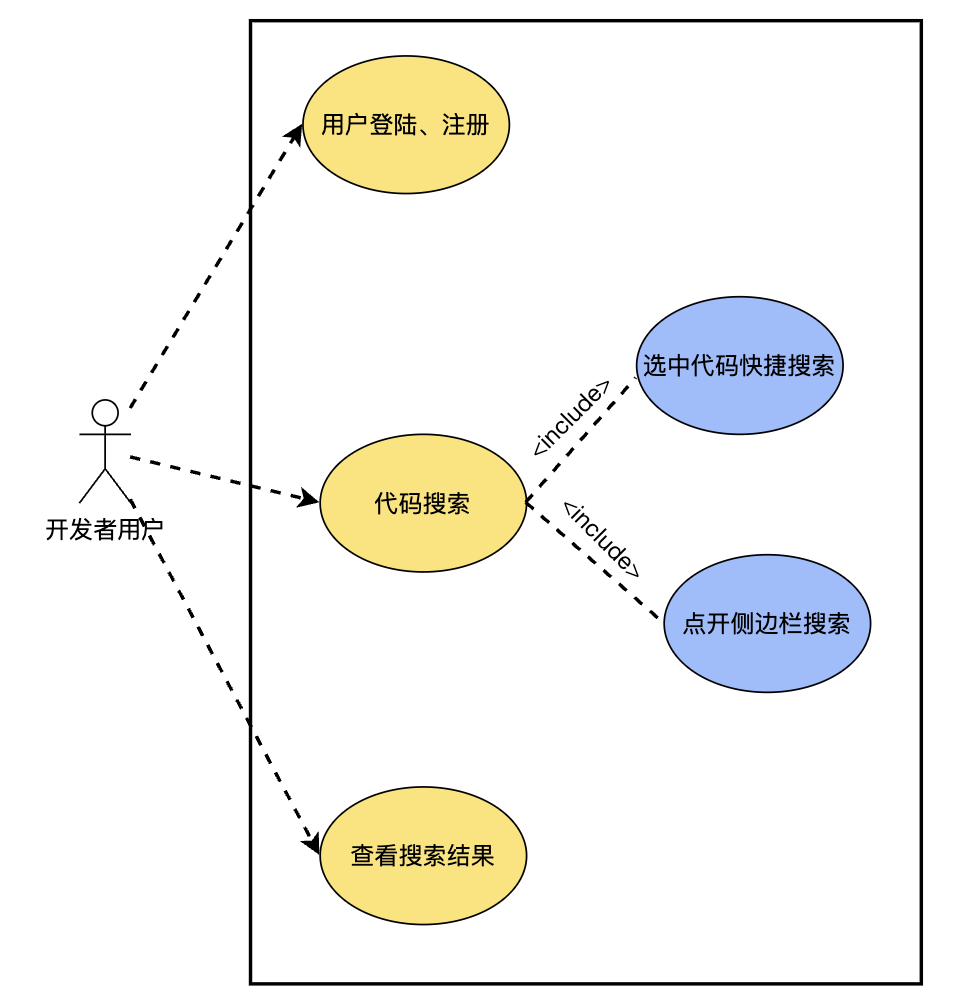
\includegraphics[width=0.95\textwidth]  {user_use.png}} 
	\caption{开发者用户用例图}
	\label{user}
\end{figure}
(1)开发者用户注册:开发者用户下载系统后,由系统弹窗提示用户在未登录状态,此时用户可以选择登录或者注册。如果用户选择注册,则跳转注册页面,用户输入邮箱号后,通过验证码自动完成注册。\par
(2)开发者用户登录:开发者用户下载系统后,由系统弹窗提示用户在未登录状态,此时用户可以选择登录或者注册。如果用户选择登录,则跳转登录页面,用户输入绑定邮箱后,经过验证,成功完成登录。\par
(3)代码搜索:开发者用户在使用VS Code编码过程中,可以通过绑定的快捷键,直接跳转搜索界面。如果此时鼠标选中了代码,则自动将代码复制到用户的系统粘贴面板上;用户也可以点击侧边的插件icon,跳转到搜索界面,手动输入搜索关键词开始搜搜。\par
(4)查看搜索结果,用户在搜索完成后,如果有搜索结果,可点击搜索结果框,通过链接自动跳转项目详情。\par
对于运维人员,做如下功能分析,图\ref{operator}为运维人员的功能需求用例图:\par
\begin{figure}[H]
	\center{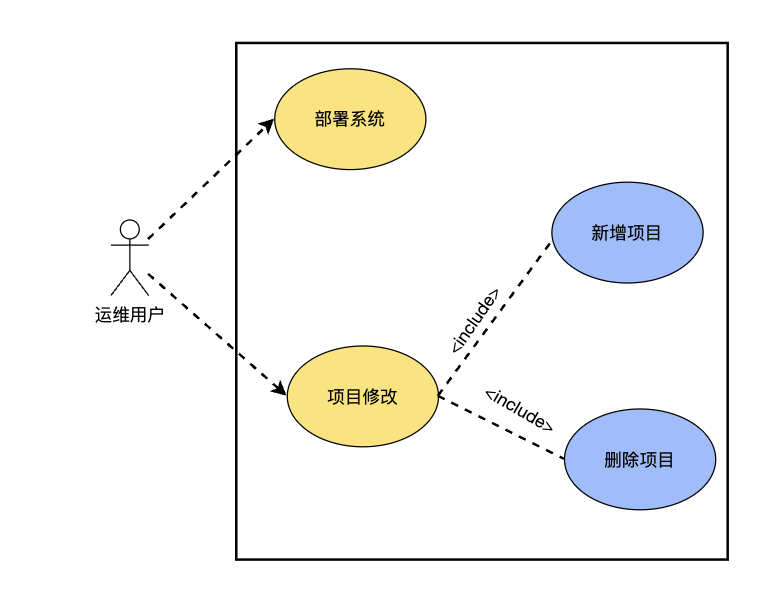
\includegraphics[width=0.95\textwidth]  {operator_user.png}} 
	\caption{运维用户用例图}
	\label{operator}
\end{figure}
(1)系统部署:运维人员能根据系统提供的指示,安装系统必要的依赖,完成系统的部署、迁移。\par
(2)项目修改:运维人员能根据项目变动,灵活新增或者删除Elasticsearch中管理的项目。\par
\subsubsection{系统非功能性需求分析}
(1)	易用性:本系统在界面布局上应当符合使用者的实际习惯与需求,应具备逻辑性和直观性,用户在进行操作时应该能够清晰地了解每个功能的用途和位置,操作流程和反馈信息也应该及时、明确。界面应该呈现出清晰、统一的信息组织结构,将不同功能和信息分类展示,让用户能够快速获取到有用的项目信息\par
(2)	拓展性:本系统应该满足可拓展需求。在前端表现层,能够快速拓展对后续需求页面,对已使用组件做到有效复用。在后端应用层,能够满足后端需求灵活变更,对新增需求和更变需求,通过利用已有功能模板快速开发。\par
(3)	可靠性:本系统的可靠性需求,主要体现在用户登录、项目搜素,大模型改写方面。具体来说,系统需要保障可靠的用户登录体验;实现可靠的搜索体验;大语言模型在改写用户提示词的时候应该确保不随意篡改用户的本意,达到提升搜索准确性等效果。\par
(4)	安全性:本系统在安全性上,做到用户间严格分离,不可跨越权限操作。需要设计具备数据备份、恢复功能的数据库处理方法,保障数据库信息安全。\par
\section{面向多编程语言的代码检索系统方案设计}
\subsection{系统总体架构设计}
面向多编程语言的代码检索系统整体将采用前后端分离的方式进行组织。可以分为前端交互层、后端逻辑层以及数据层三个维度,如图\ref{all_structure}所示。前端交互层使用Vue框架编写交互逻辑,使用ElementUI渲染前端图形化页面和可视化模块。后端使用Gin框架编写应用服务,规范API风格,接受前端请求,同时负责和数据层和大语言模型进行交互,实现主要的搜索逻辑。数据层使用Elasticsearch管理所有的项目数据。
\begin{figure}[H]
	\center{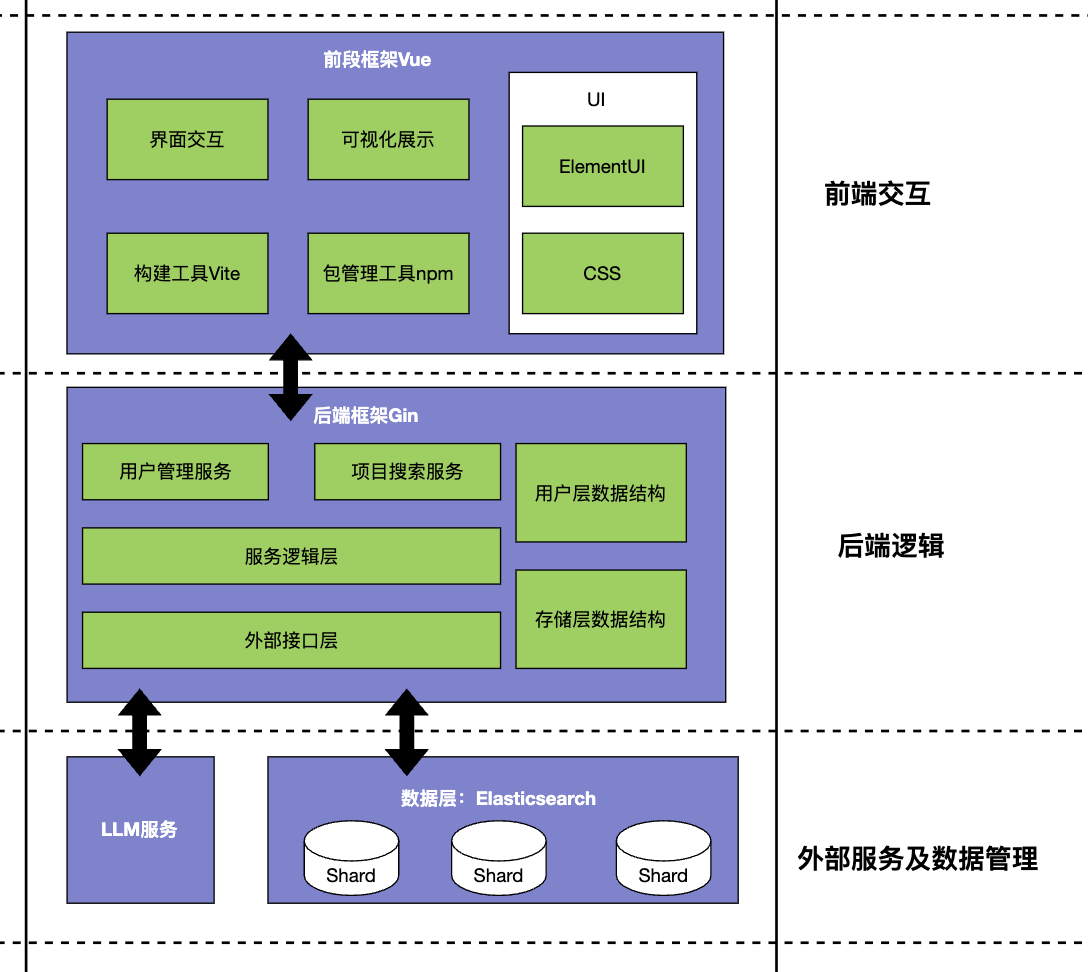
\includegraphics[width=0.95\textwidth]  {structure.png}} 
	\caption{系统总体架构图}
	\label{all_structure}
\end{figure}
\subsection{基于AST的编程语言预处理过程}
在多编程语言代码检索与理解系统中,源代码的结构化表示对于提升模型的语义理解能力和检索精度具有至关重要的作用。AST,作为编程语言语法结构的标准化表达方式,能够有效揭示代码的层次结构与语义关系。基于AST的预处理过程,旨在将原始源代码转化为统一、结构化的中间表示,为后续的特征提取、语义分析及跨语言对齐等任务奠定坚实基础。为此,本文采用了主流开源AST解析工具,对不同编程语言的项目源代码进行统一的结构化预处理。通过AST分析,可以有效揭示代码的层次结构与语义关系,为后续的特征提取和检索任务提供坚实的数据基础。\par
\begin{figure}[H]
	\center{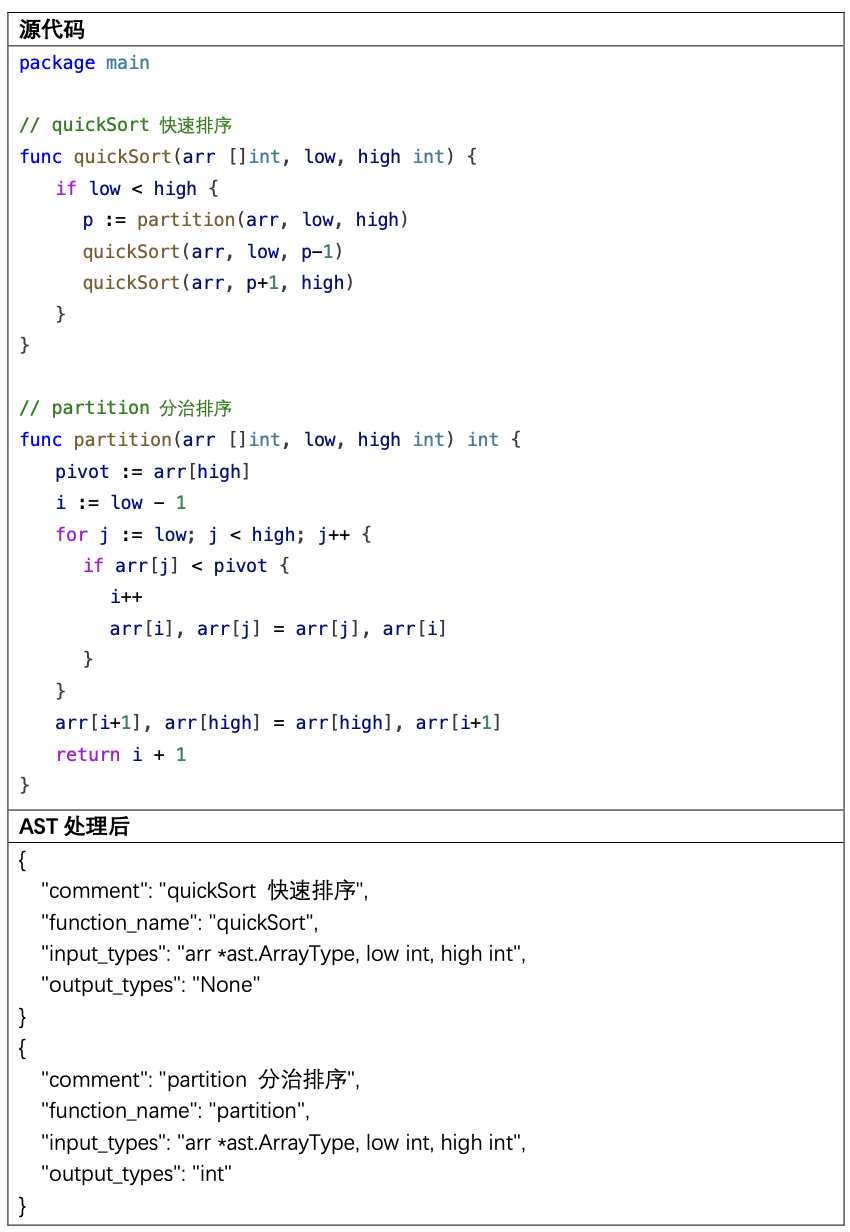
\includegraphics[width=0.95\textwidth]  {ast_example.png}} 
	\caption{AST处理示例图}
	\label{ast_example}
\end{figure}
在预处理过程中,首先,针对不同编程语言,系统调用相应的开源AST解析器,对项目源代码进行语法分析,自动生成抽象语法树。然后,系统对生成的AST进行遍历和筛选,自动去除无关的冗余信息,如单元测试代码,仅保留与核心功能实现相关的函数和代码片段。通过这一过程,极大提升了数据集的纯净度和有效性,确保后续检索模型能够聚焦于高价值的功能。此外,系统还对保留的功能函数进行了进一步的结构化处理,包括统一节点类型命名、规范化变量与函数标识符等操作,以便于多语言代码的对齐和比较。如图\ref{ast_example}所示,一段Go语言的快速排序,经过AST处理后,去除了代码中具体的递归部分,将函数的函数名以及注释和方法输入类型和输出类型提炼出来,大大规范化了这段代码在将来存储中的格式。这些经过AST预处理的数据集不仅具备良好的结构化特性,也为多编程语言代码检索系统提供了高质量的输入基础。\par
\subsection{基于微服务的高可用后台分布式技术}
随着软件系统规模的不断扩大和业务复杂度的持续提升,传统的单体式后端架构已难以满足现代多编程语言代码检索系统在高可用性、可扩展性和灵活性方面的需求。微服务架构作为当前主流的分布式系统设计范式,通过将复杂系统拆分为一组松耦合、自治的服务单元,实现了服务的独立部署、弹性扩容和高效协作,成为支撑大规模智能代码检索平台的关键技术基础。所谓微服务架构,是指将系统按照业务功能划分为多个独立的服务,每个服务围绕特定业务能力构建,拥有独立的数据存储和运行环境,并通过轻量级通信机制(本文使用gRPC协议)进行协作。与传统单体架构相比,微服务架构不仅提升了系统的可维护性和可演化性,还极大增强了系统在高并发、分布式部署和多语言支持等场景下的适应能力。在面向多编程语言的代码检索系统中,微服务架构能够有效支撑多语言解析、智能检索、权限管理等异构服务的协同运行,为系统的高可用性和弹性扩展提供坚实保障。\par
本节围绕高可用后台分布式技术的微服务架构展开,提出了一套系统化的后端设计方案。该方案以服务自治、弹性伸缩和容错机制为核心,结合分布式服务注册与发现、负载均衡、服务治理等关键技术,实现了多编程语言代码检索系统的高可用、可扩展和易维护的后端支撑平台。整体方案包括以下两个阶段:\par
(1)第一阶段为服务拆分与分布式部署。系统根据业务功能将后端划分为网关服务、鉴权服务、搜索服务、大语言模型服务等多个微服务单元。每个服务均可独立开发、测试、部署和扩容,极大提升了系统的灵活性和可维护性。通过容器化技术和分布式编排平台,各服务能够在多节点环境下弹性部署,实现资源的动态调度和高可用保障。服务间通过gRPC等高效通信协议进行数据交互,确保低延迟和高吞吐量。\par
(2)第二阶段为高可用性与服务治理机制设计。系统引入分布式服务注册与发现机制,所有微服务在启动时自动向服务注册中心,注册自身信息,其他服务可通过注册中心动态发现并调用目标服务,提升系统的灵活性和容错能力。为应对高并发和突发流量,系统在网关层集成负载均衡策略,自动分发请求至后端多实例服务,避免单点瓶颈。各服务内部实现健康检查与自动故障转移机制,确保部分节点故障时系统整体仍能稳定运行。此外,系统还支持灰度发布、自动扩缩容、日志追踪与链路监控等服务治理能力,为后续功能迭代和运维管理提供有力支撑。\par
\begin{figure}[H]
	\center{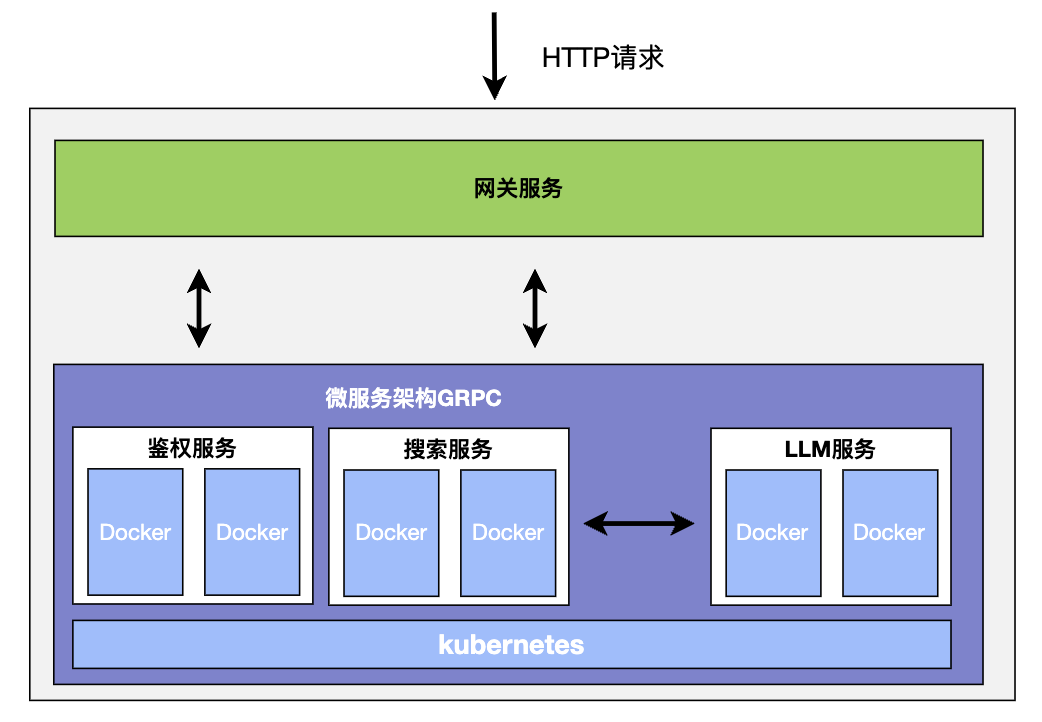
\includegraphics[width=0.95\textwidth]{back_model.png}}
	\caption{微服务架构下的高可用分布式后台结构}
	\label{microservice_arch}
\end{figure}
如图\ref{microservice_arch}所示,为面向多编程语言的代码检索系统的整体后台架构。网关统一对外提供API入口,负责请求路由、鉴权与负载均衡。鉴权服务独立负责用户注册、登录与Token校验,保障系统安全。搜索服务与大语言模型服务协同,实现多语言代码的查询上下文增强以及智能检索。所有服务均支持多实例部署,结合容器编排平台实现弹性扩容和自动恢复,显著地提升系统的高可用性和并发处理能力。\par
\subsection{微服务系统中的统一接入与安全网关服务}
在基于微服务的分布式系统中,服务网关是保证整体服务安全、可扩展性与高可用性的核心基础设施之一。所谓服务网关,是指在分布式微服务系统中,作为所有外部请求的统一入口,负责流量调度、统一鉴权、安全防护、协议转换等多重关键任务。与传统单体系统的直接访问模式不同,服务网关通过集中管理和智能路由,有效屏蔽了后端服务的复杂性,提升了系统的安全性、灵活性和运维效率。在面向多编程语言的代码检索系统中,网关机制不仅承担着请求分发和安全防护的基本职责,更需要适应多语言、多协议和高并发的复杂业务场景,从而保障系统整体的稳定运行和高效服务能力。\par
\begin{figure}[H]
	\center{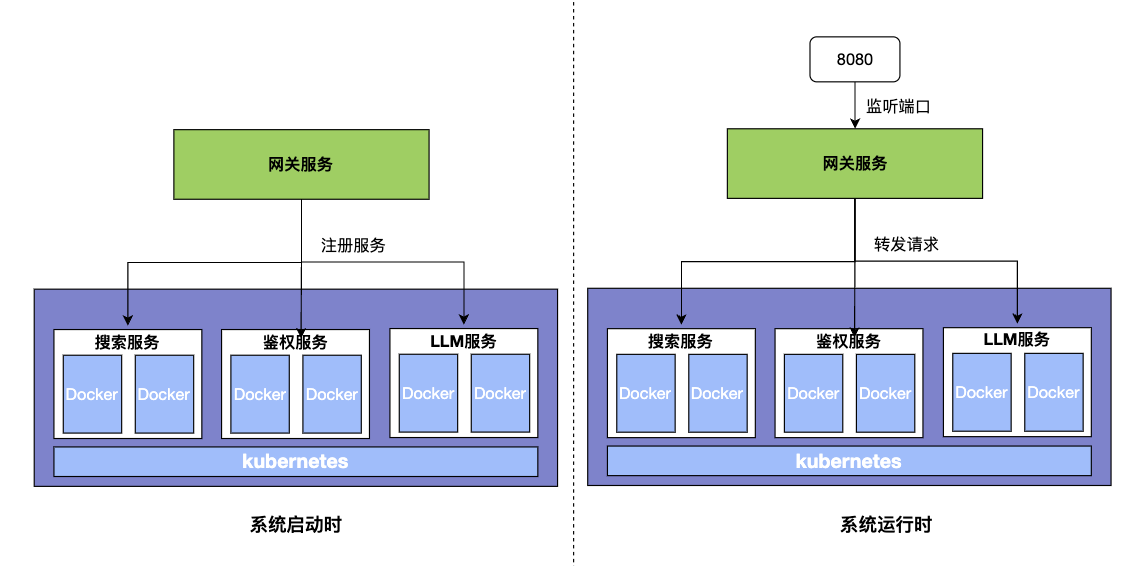
\includegraphics[width=0.95\textwidth]  {gateway.png}} 
	\caption{网关工作原理图}
	\label{gateway}
\end{figure}
在面向多编程语言的代码检索系统中,网关服务基于Gin框架,基本实现了服务的统一注册,均衡路由以及服务鉴权等功能。图\ref{gateway}为本服务的网关服务的简单工作原理图示例。网关的工作过程分为服务启动时和服务运行时两个阶段。在在服务启动时,网关会向鉴权服务、搜索服务和大语言模型服务发送探活请求,确保系统内所有服务都能够正常连接。在服务运行时,网关服务监听服务器的特定端口。在本系统中,网关监听8080端口,所有的请求经过网关集成的多种负载均衡策略(如轮询、最少连接等)之一,根据实时流量和服务健康状态,智能分发至后端对应的微服务实例。同时,对于所有的请求,都将经过鉴权服务鉴权,确保请求访问的权限在安全控制范围呢。\par
\subsection{微服务系统中的统一身份认证与安全鉴权服务}
在现代微服务系统中,统一身份认证与安全鉴权机制是保障系统安全性、数据完整性与用户隐私的核心基础设施。所谓鉴权服务,是指在多服务协同的分布式系统中,专门负责用户身份验证、权限校验及会话管理的独立服务模块。与传统单体系统中嵌入式的认证方式不同,分布式鉴权系统通过集中式管理和标准化接口,有效提升了系统的安全性、可扩展性和运维效率,并且往往依赖分布式数据库解决统一路由问题。在面向多编程语言的代码检索系统中,鉴权服务不仅承担着用户注册、登录与会话管理的基本职责,更需适应高并发环境下的复杂业务场景,从而为系统的安全运行和用户体验提供坚实保障。
\begin{figure}[H]
	\center{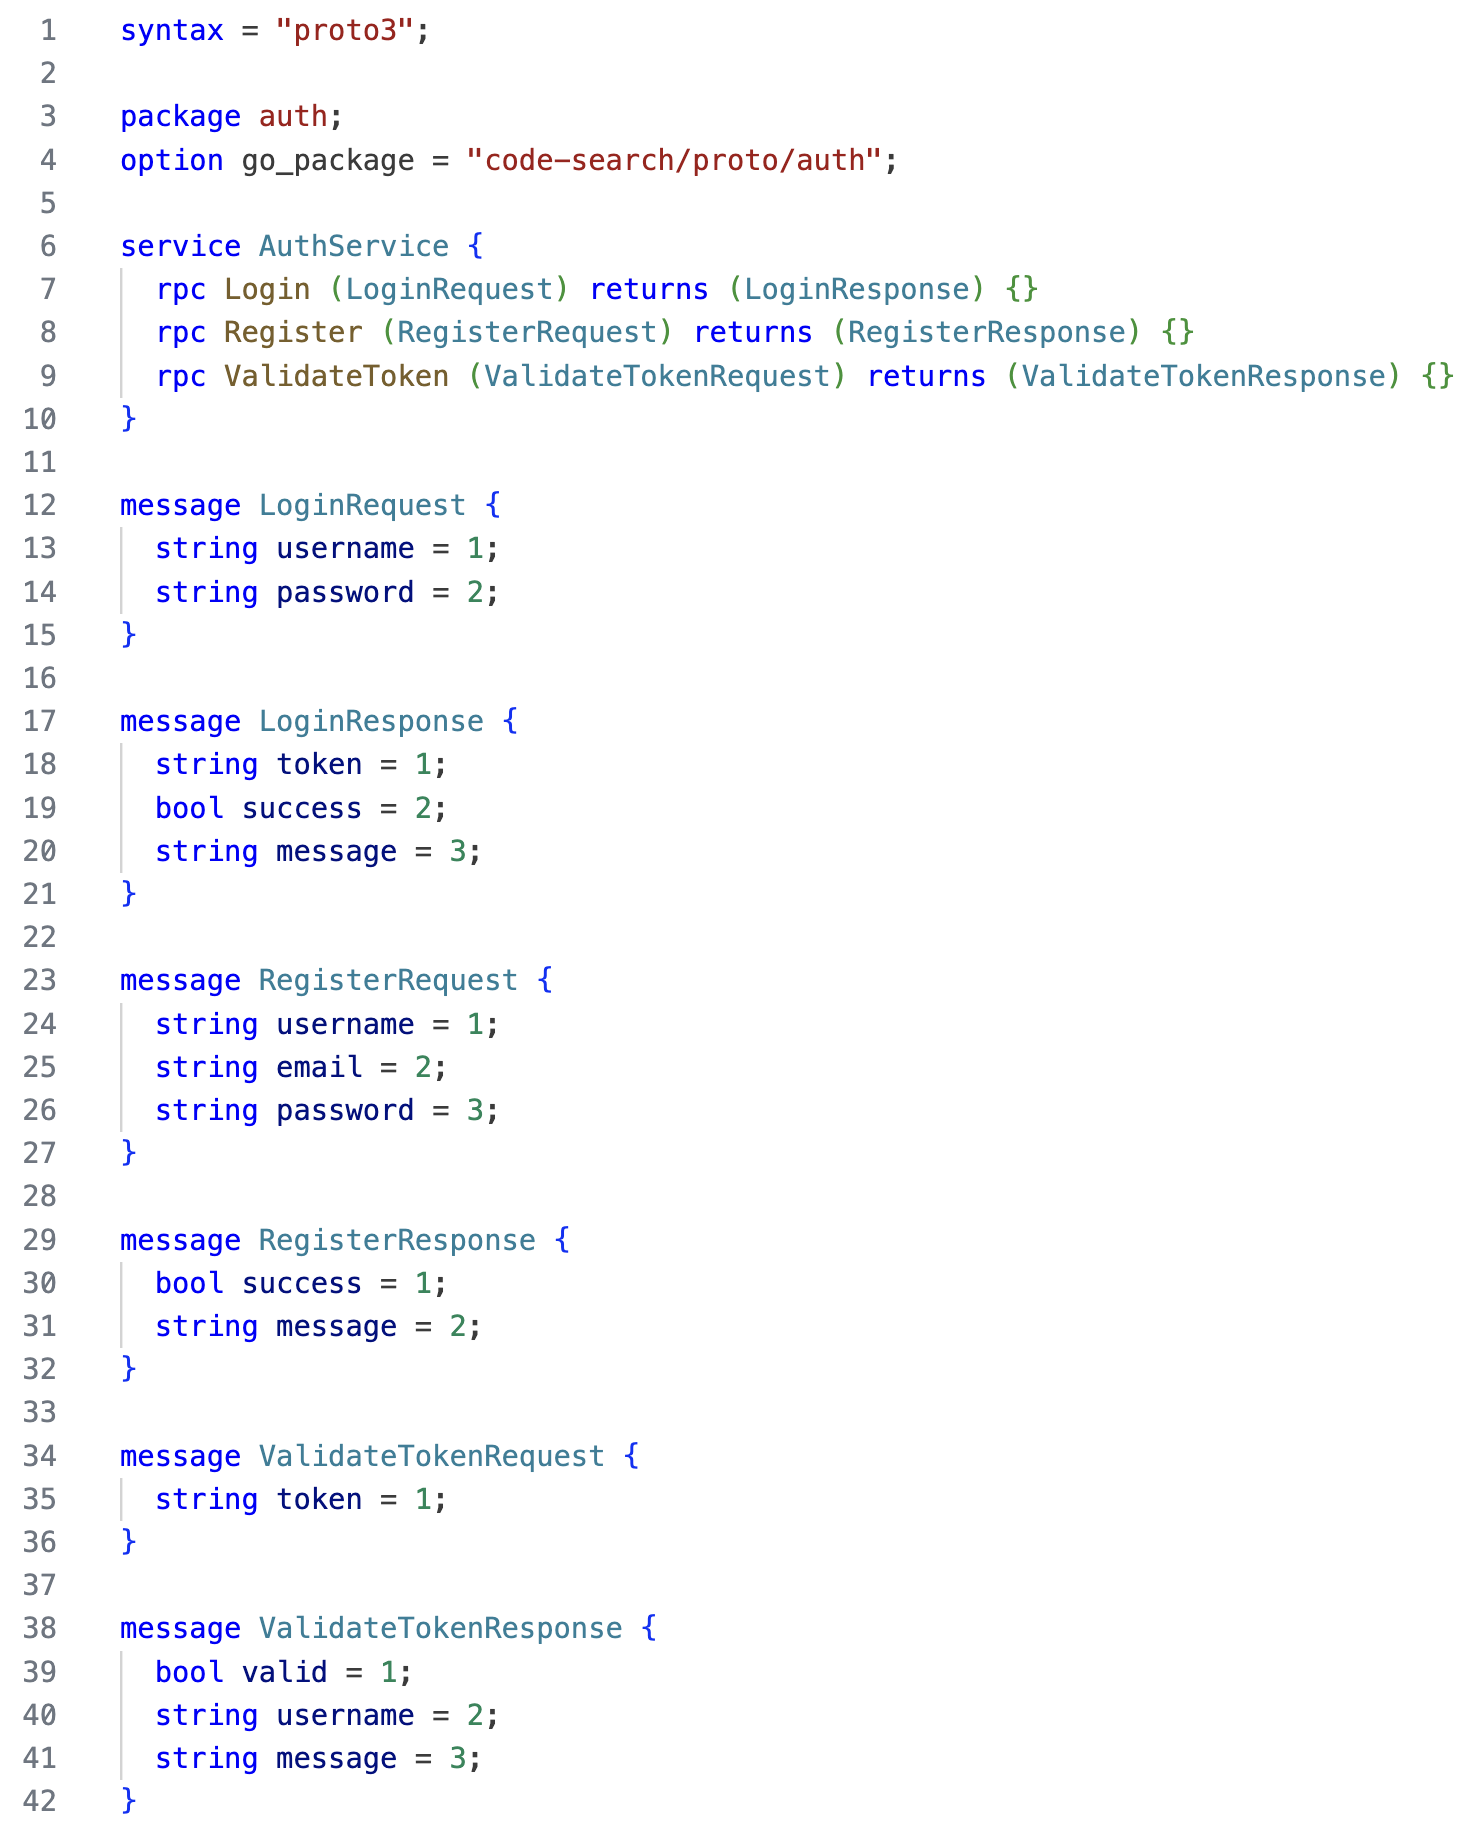
\includegraphics[width=0.95\textwidth]  {proto.png}} 
	\caption{鉴权服务协议}
	\label{auth}
\end{figure}
本系统的统一身份认证与安全鉴权机制基于gRPC高性能通信框架实现,采用标准化的proto协议(如图\ref{auth}所示)定义服务接口,确保各微服务间的高效互操作与安全通信。整体流程涵盖用户注册、登录认证与会话状态校验等核心环节,如图\ref{auth_flow}所示,具体包括以下三个阶段:\par
\begin{figure}[H]
	\center{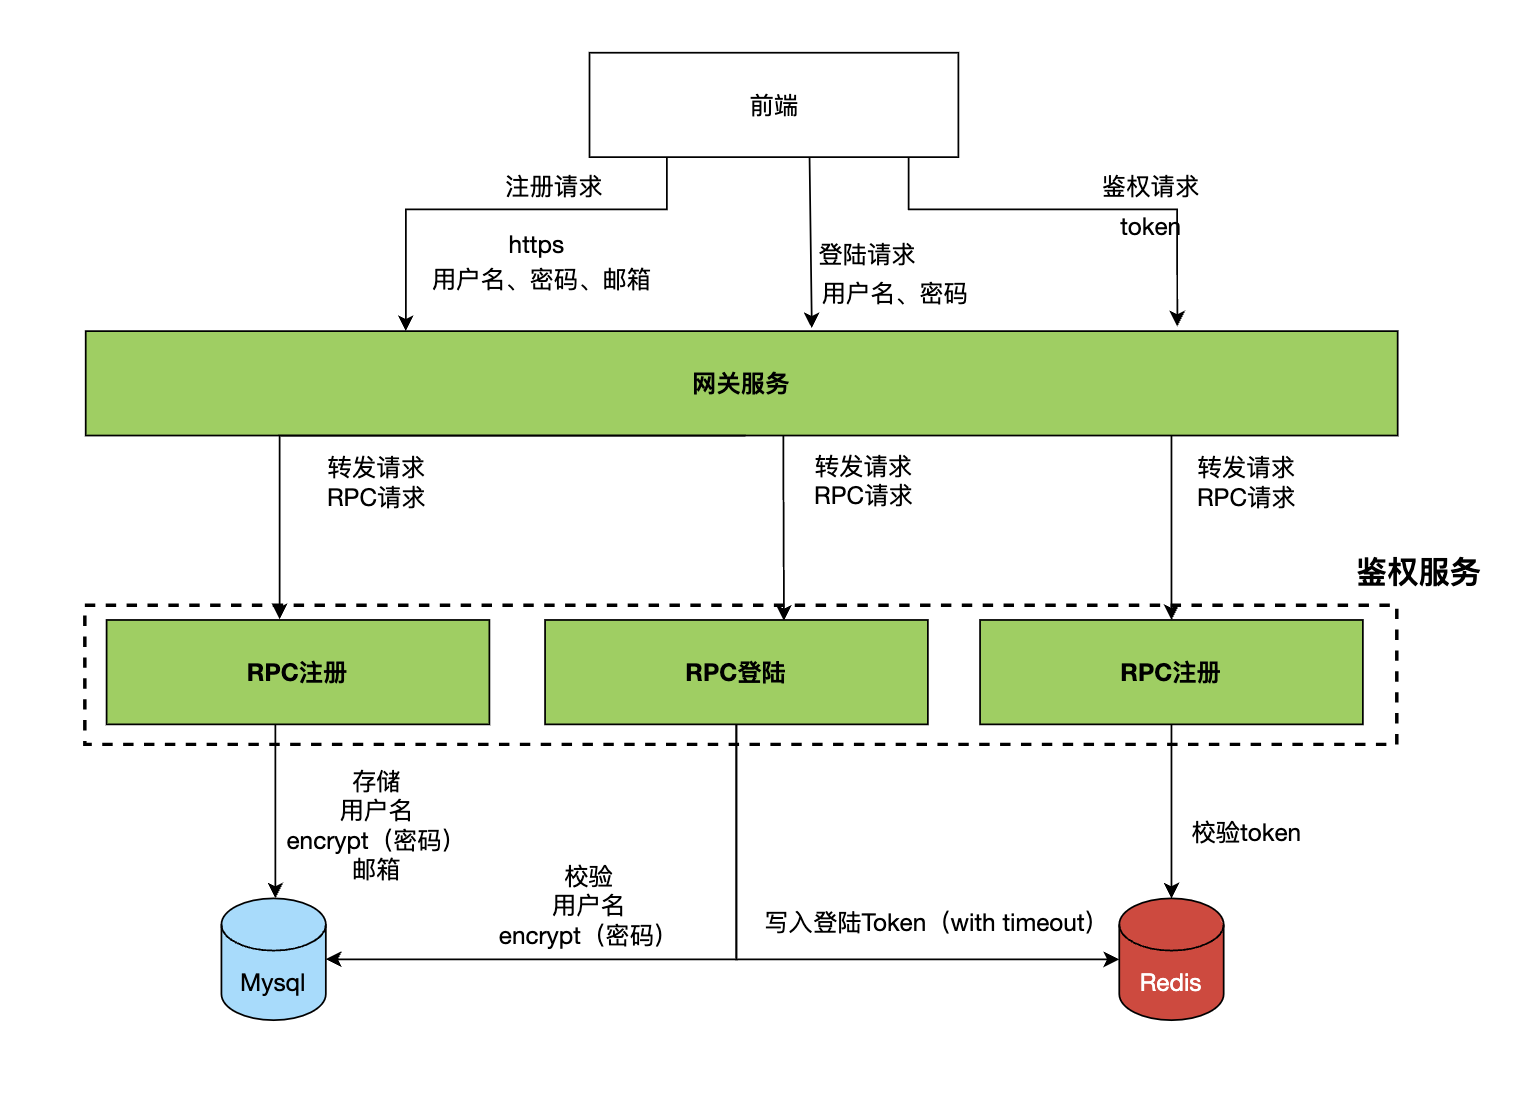
\includegraphics[width=0.95\textwidth]{auth.png}}
	\caption{统一身份认证与鉴权服务工作原理}
	\label{auth_flow}
\end{figure}
第一阶段为用户注册与身份信息安全存储。用户通过前端界面提交用户名、邮箱及密码等注册信息,所有注册请求均通过HTTPS协议加密传输至服务网关,从而防止敏感数据在传输过程中被窃取。服务网关对请求进行初步校验后,将其转发至鉴权服务的注册接口。为进一步保障用户密码安全,系统采用哈希加密算法对密码进行不可逆处理,最终将加密后的密码存储于数据库中。即使数据库遭受攻击,用户的原始密码信息也无法被直接获取,有效提升了系统的抗攻击能力。用户注册信息表如表\ref{usertable}所示,其中id字段作为用户的唯一标识符,由系统使用雪花算法自动生成。雪花算法是一种高效且广泛认可的ID生成方案,能够在本项目的用户基数和并发量下充分保证ID的唯一性。用户名(username)、电子邮件(email)及密码(password)字段则用于用户的注册和认证过程,且密码在存储前均经过哈希加密处理,从而在数据传输和存储环节进一步保障了用户信息的安全性。\par
\begin{table}[H]
	\centering
	\caption{用户信息表(code\_search\_user)}
	\small
	\begin{tabular}{c c c c}
		\toprule
		列名 & 数据类型 & 主键 & 注释\\
		\midrule
		id & bigint & 是 & 用户ID(通过雪花算法自动生成)\\
		username & varchar(255) & 否 & 用户名\\
		email & varchar(255) & 否 & 用户电子邮件地址\\
		password & varchar(255) & 否 & 用户密码(采用哈希加密存储)\\
		\bottomrule
	\end{tabular}
	\label{usertable}
\end{table}
第二阶段为用户登录与会话令牌(Token)分发。用户通过输入用户名和密码发起登录请求,系统在接收到请求后,对用户提交的凭证进行哈希校验。认证通过后,鉴权服务为用户生成唯一的会话Token,并将该Token安全存储于分布式Redis集群中。此后,用户在访问系统各项服务时,均需携带该Token以证明其身份合法性。Token机制不仅提升了系统的安全性,还便于实现分布式环境下的无状态会话管理。\par
第三阶段为会话状态检测与权限校验。每当用户发起请求时,需在请求头中携带有效的Token。服务网关在接收到请求后,首先将Token转发至鉴权服务进行有效性校验。鉴权服务通过验证Token的合法性及其在Redis集群中的存在性或是否超时淘汰判断用户会话是否有效。若校验通过,网关将放行请求并转发至目标微服务;若校验失败,则拒绝请求并返回相应的错误信息。该机制有效防止了未授权访问和会话劫持等安全风险,保障了系统的整体安全性和稳定性。
\subsection{基于高性能分布式查询引擎的代码查询服务}
在面向多编程语言的代码检索系统中,基于分布式的高性能查询引擎是实现高效、精准检索体验的核心功能模块。该服务基于前期AST的预处理,并且依赖LLM对用户查询意图的深度理解与重写,结合Elasticsearch高性能检索引擎最终完成了高效的代码查询与结果排序。本章节将介绍查询服务的整体任务流程,并重点介绍高性能分布式查询引擎Elasticsearch在本项目中的具体使用情况。\par
该服务基于gRPC高性能远程过程调用框架实现,采用protobuf协议定义标准化的服务接口,协议如图\ref{search_proto}所示。\par
\begin{figure}[H]
	\center{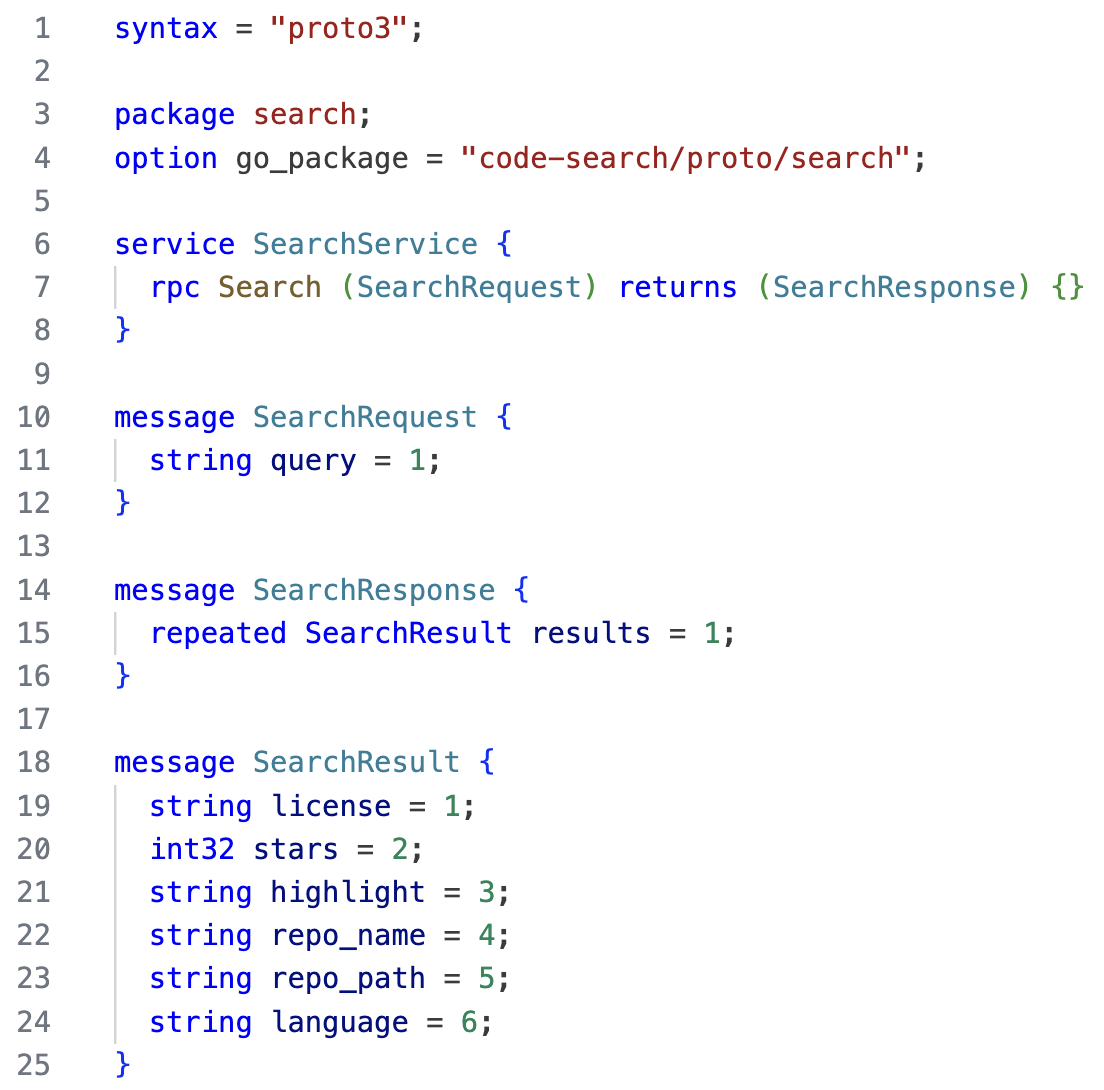
\includegraphics[width=0.95\textwidth]{search_proto.png}}
	\caption{智能搜索服务协议}
	\label{search_proto}
\end{figure}
用户的检索请求通过Search接口提交,SearchRequest与SearchResponse分别定义了请求与响应的数据结构。其中,SearchResponse结构体包含SearchResult列表,用于承载多样化的检索结果,支持多语言、多协议和多维度的代码查询需求。系统整体的用户搜索流程如图\ref{timeline}所示,用户经过鉴权后提交检索请求,系统将用户的原始查询语句发送至模型侧。模型对用户查询意图进行深度理解与专业化改写,并将优化后的检索词返回给查询系统。系统再将经过大模型处理的检索请求发送至底层数据库,数据库返回查询结果,最终由系统进行可视化展示。\par
\begin{figure}[H]
	\center{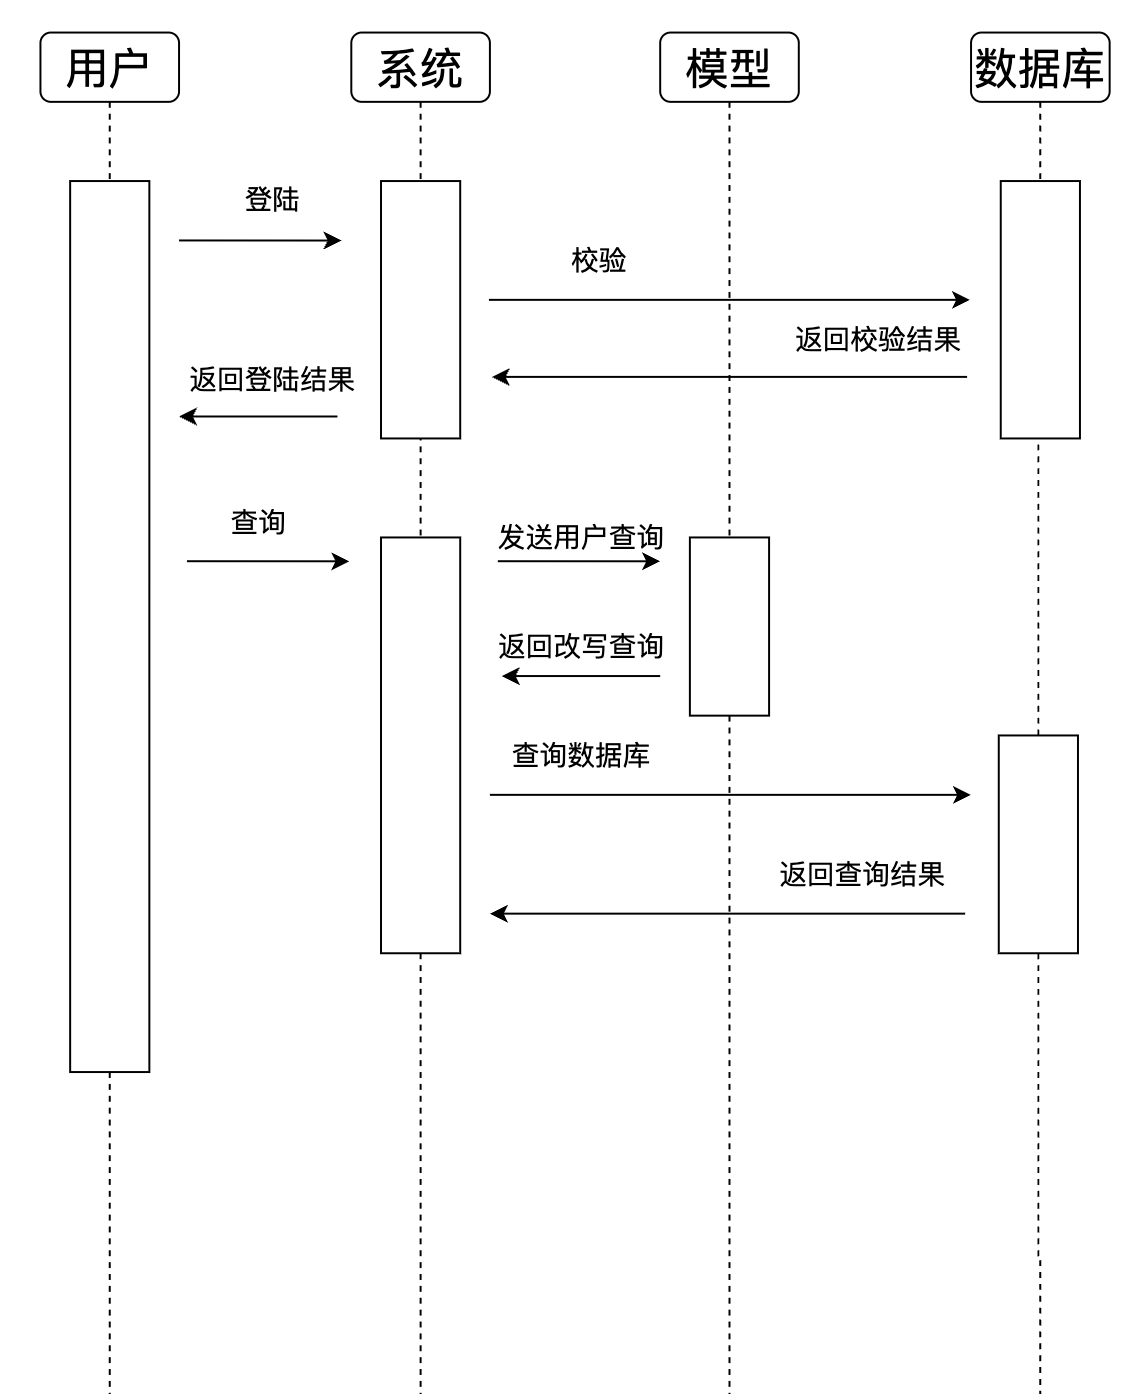
\includegraphics[width=0.95\textwidth]{timeline.png}}
	\caption{用户搜索时序图}
	\label{timeline}
\end{figure}
Elasticsearch作为底层分布式检索引擎,承担着代码数据的高效存储、索引与查询任务。为满足多语言、多协议、多维度的检索需求,系统在Elasticsearch中为代码数据设计了结构化的Mapping,如表\ref{esmapping}所示。
\begin{table}[H]
	\centering
	\caption{索引code的映射结构}
	\label{tab:code_mapping}
	\small
	\begin{tabular}{c c c}
		\toprule
		字段名 & 数据类型 & 描述 \\
		\midrule
		content & text & 代码内容(文本类型) \\
		file\_name & keyword & 文件名(关键字类型) \\
		repo\_name & keyword & 文件所属项目名(关键字类型)\\
		lang & keyword & 编程语言(关键字类型) \\
		lic & keyword & 许可证类型(关键字类型) \\
		stars & integer & 星标数量(整数类型) \\
		\bottomrule
	\end{tabular}
	\label{esmapping}
\end{table}
在该Mapping结构中,content字段采用text类型,支持分词和全文检索,能够对代码内容进行高效的语义匹配和相关性排序。file\_name和repo\_name字段采用keyword类型,便于对特定文件或项目进行精确过滤和聚合统计,同时也方便在搜索结果中展示文件和项目的详细信息。lang字段用于标识代码所使用的编程语言,lic字段记录代码的开源协议类型,这两个字段均为keyword类型,能够支持高效的条件过滤和多维度聚合分析。stars字段则记录项目的星标数量,采用integer类型,便于对检索结果进行数值排序和统计分析,例如优先展示高星项目或实现项目热度排行。基于上述Mapping结构,系统能够灵活支持多维度的检索需求。在实际查询流程中,服务端会根据LLM生成的结构化检索指令,将用户的查询意图映射到Elasticsearch的复合查询语句中,从而提升查询的联想能力以及准确性。
\subsection{基于提示词工程的查询上下文增强技术}
随着大语言模型在自然语言处理和代码智能领域的广泛应用,提示词工程逐渐成为提升模型性能和用户体验的关键技术之一。所谓提示词工程,是指针对特定任务或应用场景,系统性地设计、优化和管理输入给大语言模型的提示,以引导模型生成更符合预期的输出结果。与传统的模型训练和微调方法不同,提示词工程无需对模型参数进行修改,而是通过调整输入内容和结构,充分挖掘和利用预训练模型的知识和推理能力。在基于大语言模型的多编程语言代码检索系统中,提示词的设计与优化对检索效果具有决定性影响。尤其是在处理跨语言、跨领域的复杂检索需求时,提示词不仅承担着任务指令的基本职责,更需要有效整合用户意图、上下文信息以及目标语言特性,从而提升模型对查询语义的理解能力和检索结果的相关性。本节围绕查询上下文增强的提示词工程展开,提出了一套系统化的提示词设计流程。该流程的核心在于以结构化上下文信息为中介桥梁,实现用户自然语言查询与多语言代码语料之间的高效对接。整体流程包括两个阶段:\par
第一阶段为查询意图解析与上下文信息提取。系统首先对用户输入的原始检索词进行语义分析,识别其中的功能需求、目标编程语言、相关API或库等关键信息。同时,结合用户历史检索记录、当前项目上下文等外部信息,自动补全或纠正不完整、模糊的查询表达。该阶段输出结构化的查询意图数据,为后续提示词生成提供事实性基础。\par
第二阶段为提示词模板生成与大模型推理。系统将解析得到的结构化查询意图与用户原始检索词一并输入,通过精心设计的提示词模板,引导大语言模型进行代码检索。该阶段的目标是融合用户需求、上下文信息与目标语言特性,提升模型对检索意图的理解深度和检索结果的准确性。\par
\begin{figure}[H]
	\center{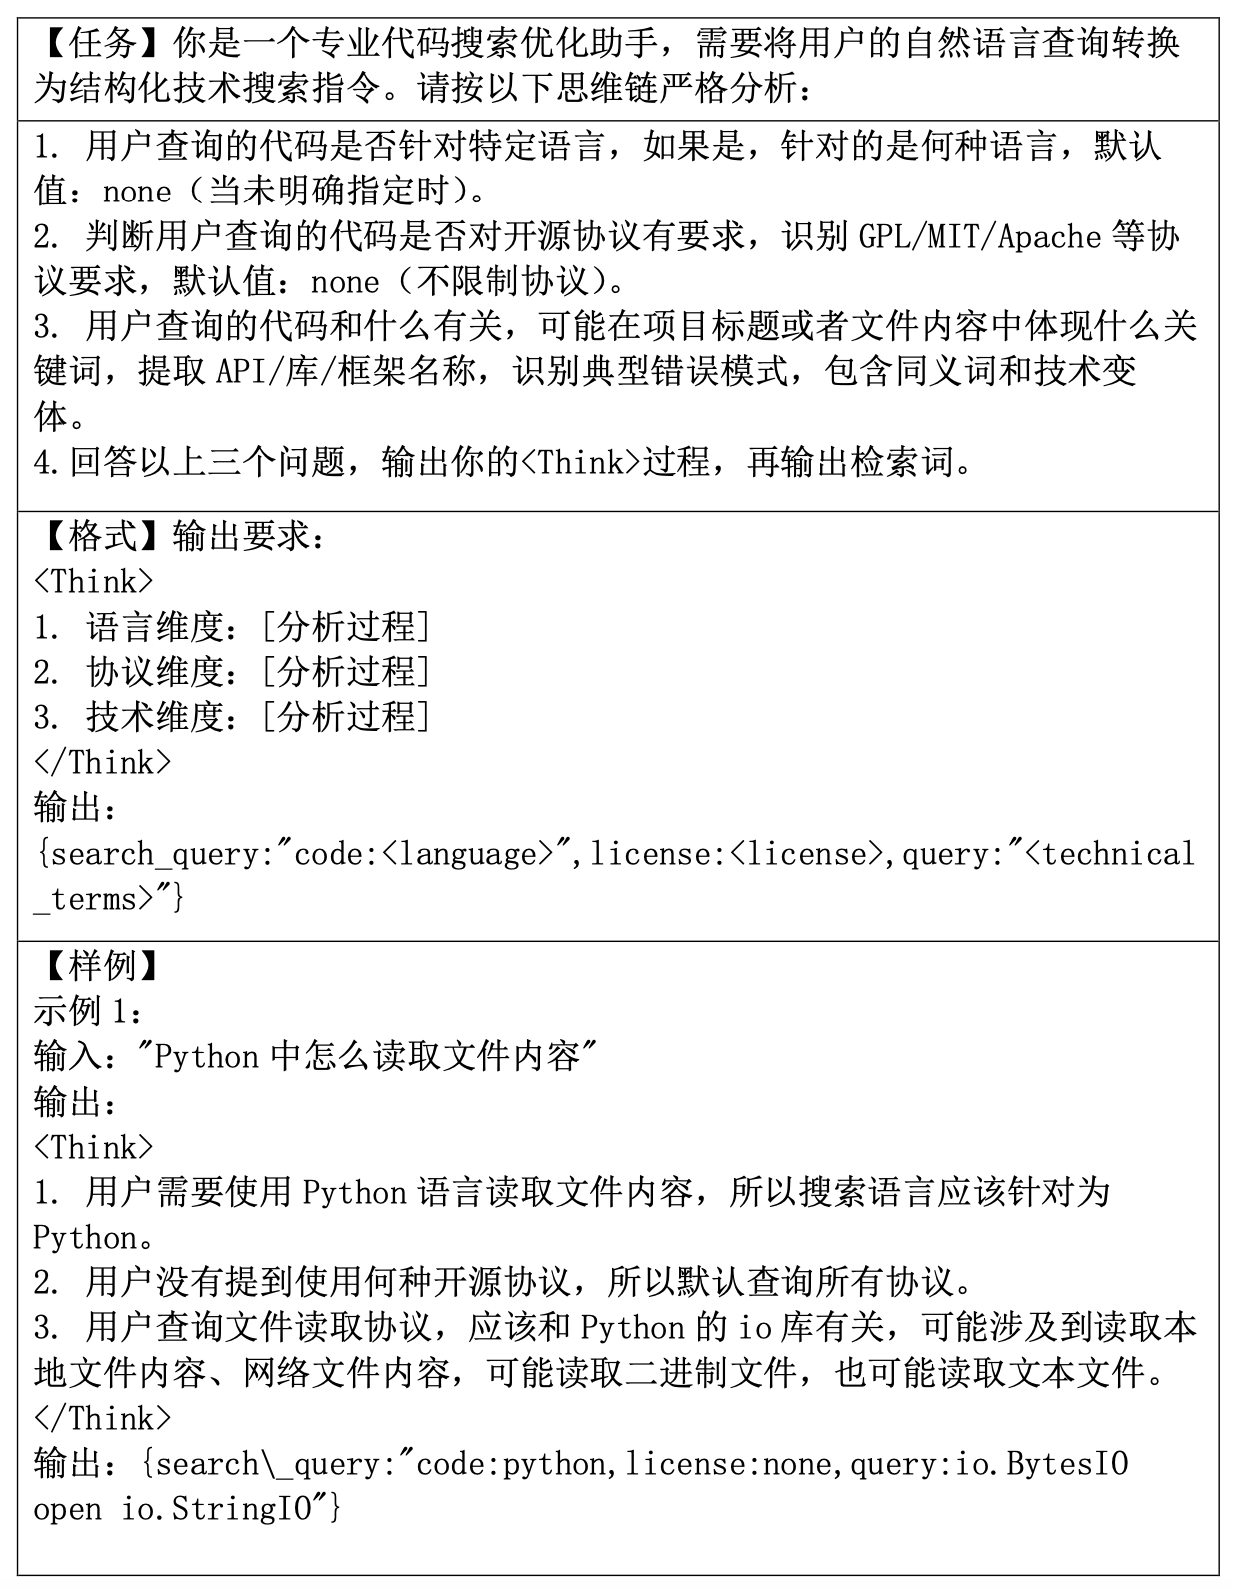
\includegraphics[width=0.95\textwidth]  {prompt1.png}} 
	\caption{提示词结构}
	\label{prompt1}
\end{figure}
\begin{figure}[H]
	\center{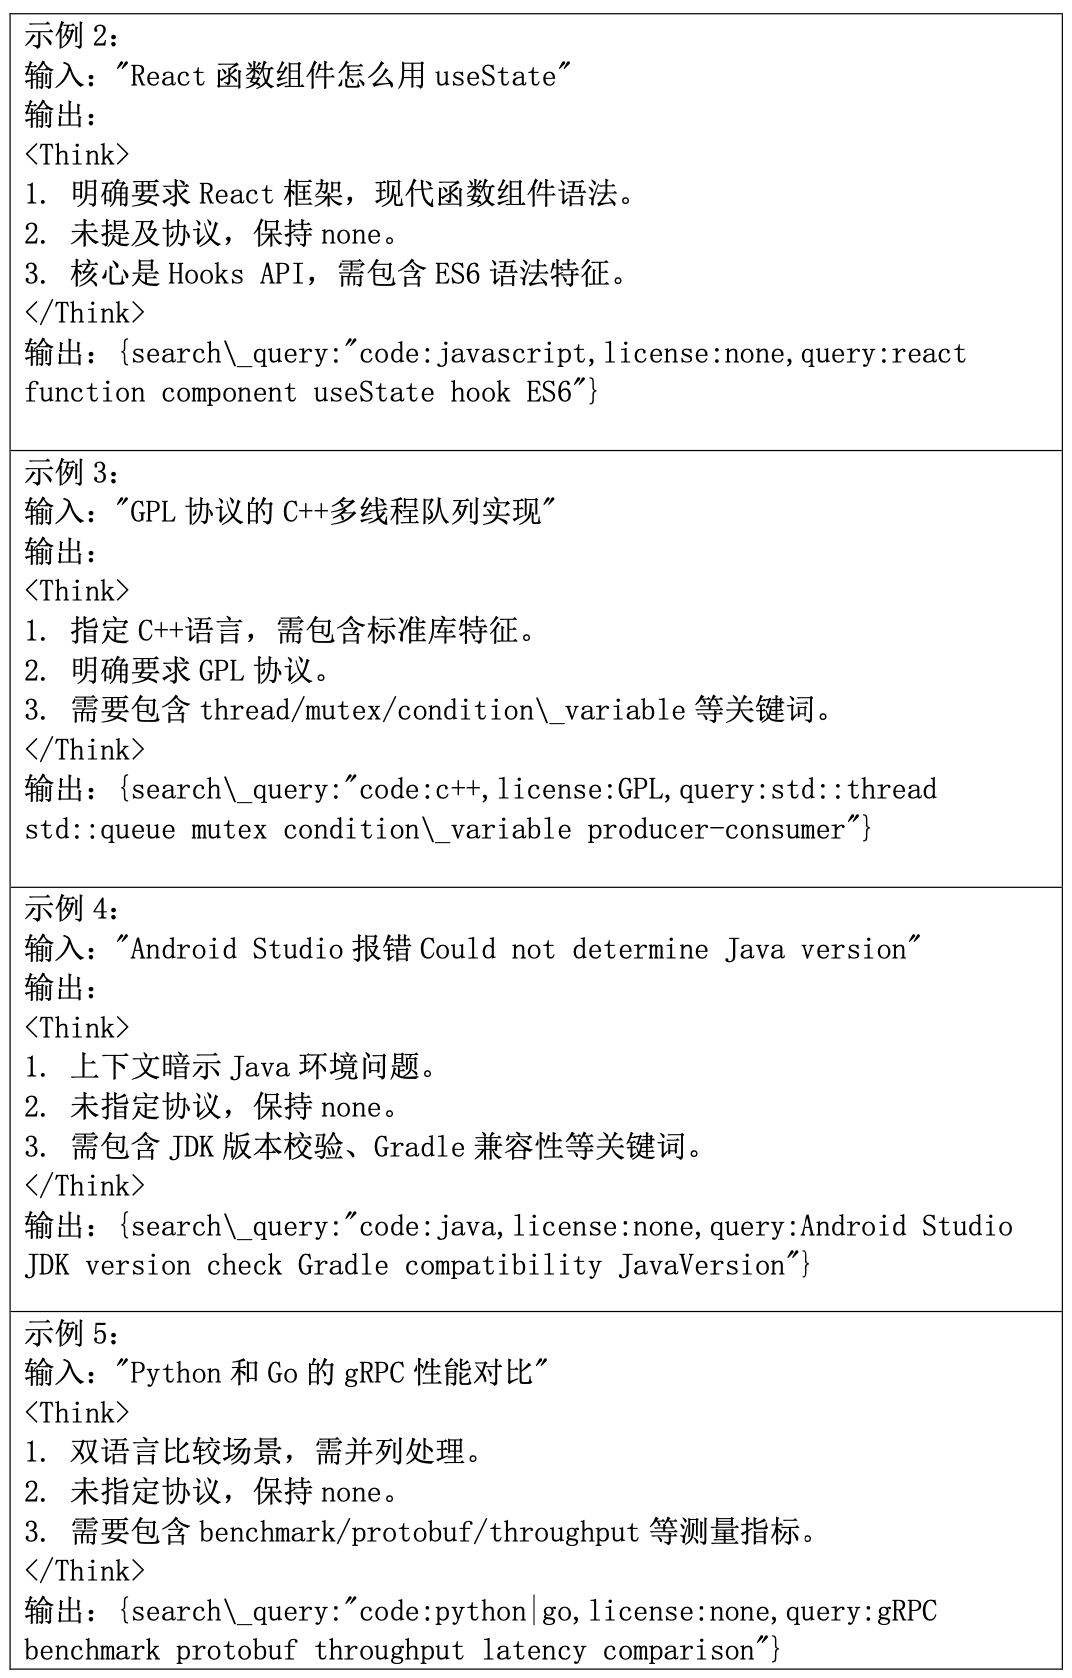
\includegraphics[width=0.95\textwidth]  {prompt2.png}} 
	\caption{提示词结构}
	\label{prompt2}
\end{figure}
为实现上述目标,本文设计了一种多层次的提示词模板,其基本结构如图\ref{prompt1}所示。该结构以“任务-思维链-结构化输出”为核心,系统性地分解和重构用户的自然语言查询。具体而言,提示词首先引导大语言模型依次分析语言、协议、技术三个维度,既能够捕捉用户的显性需求,也能挖掘隐含的上下文信息和技术细节。模型需判断查询是否针对特定编程语言,并据此设定检索范围;其次,识别用户对开源协议的潜在要求,确保检索结果的合规性;最后,深入分析与查询相关的API、库、框架及典型技术关键词,提升检索的专业性和覆盖面。在输出格式上,提示词模板采用<Think>标签对模型的推理过程进行显式分层,要求模型分别阐述对每一维度的分析思路,增强推理的可解释性和透明度。最终,系统将分析结果以结构化的JSON格式输出,明确标注检索语言、协议要求及技术关键词,为后续的代码检索模块提供高质量、可直接执行的查询指令。\par
进一步地,如图\ref{prompt2}所示,本文引入了few-shot示例驱动的提示词工程方法。通过在提示词模板中配备多样化的输入输出示例,涵盖单语言检索、框架API查询、协议限定、错误诊断及多语言对比等典型场景,模型能够更好地学习如何将复杂、模糊的自然语言需求转化为精确、结构化的检索表达。few-shot示例不仅为模型提供了明确的任务范式和推理参考,还显著提升了模型在多编程语言代码检索任务中的理解能力和检索准确率。通过这种“任务-思维链-结构化输出”的提示词工程方法,系统能够有效适应多样化的用户需求,提升整体检索性能和用户体验。
\subsection{智能代码检索系统前端架构与界面设计}
本系统前端交互界面采用基于Vue框架的MVVM(Model-View-ViewModel)架构模式,将整体结构划分为视图层(View)、视图模型层(ViewModel)和模型层(Model)三个部分。前端系统架构如图\ref{front_model}所示。视图层负责呈现用户界面,承载所有用户交互操作。主要包括开发者的注册与登录界面、代码检索页面、检索结果展示页面等功能模块;视图模型层负责前端业务逻辑的处理,是连接视图层与模型层的桥梁。该层实现了账户注册与登录、代码搜索、项目详情展示等核心逻辑,并负责响应用户操作、更新界面状态;模型层主要用于前端数据的临时存储和状态管理。该层对视图模型层传递的数据进行缓存,并实现对数据变化的监听与响应,确保界面数据的实时同步和一致性。
\begin{figure}[H]
	\center{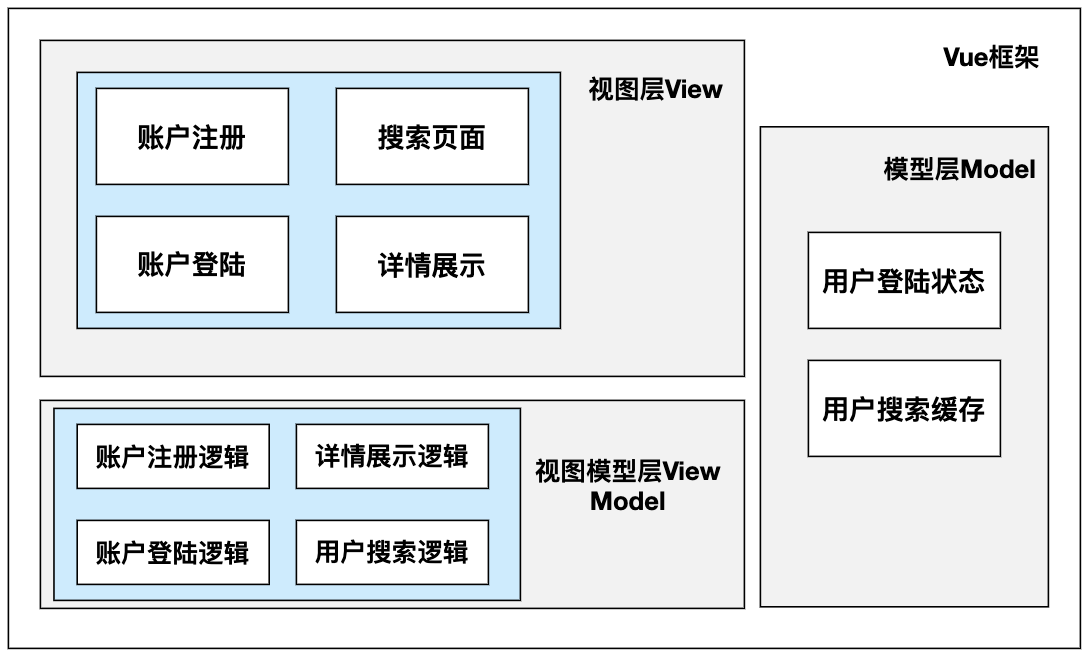
\includegraphics[width=0.95\textwidth]{front_model.png}}
	\caption{前端系统架构图}
	\label{front_model}
\end{figure}
系统支持通过VS Code插件进行代码检索,极大提升了用户的使用便捷性。插件依托VS Code提供的 \texttt{vscode.WebviewViewProvider} 接口开发,将前端Web页面无缝集成到VS Code左侧Tab栏。用户只需点击Tab栏按钮,即可进入代码搜索界面,体验与Web端一致的检索与结果展示功能。插件界面如图\ref{vscode}所示。
\begin{figure}[H]
	\center{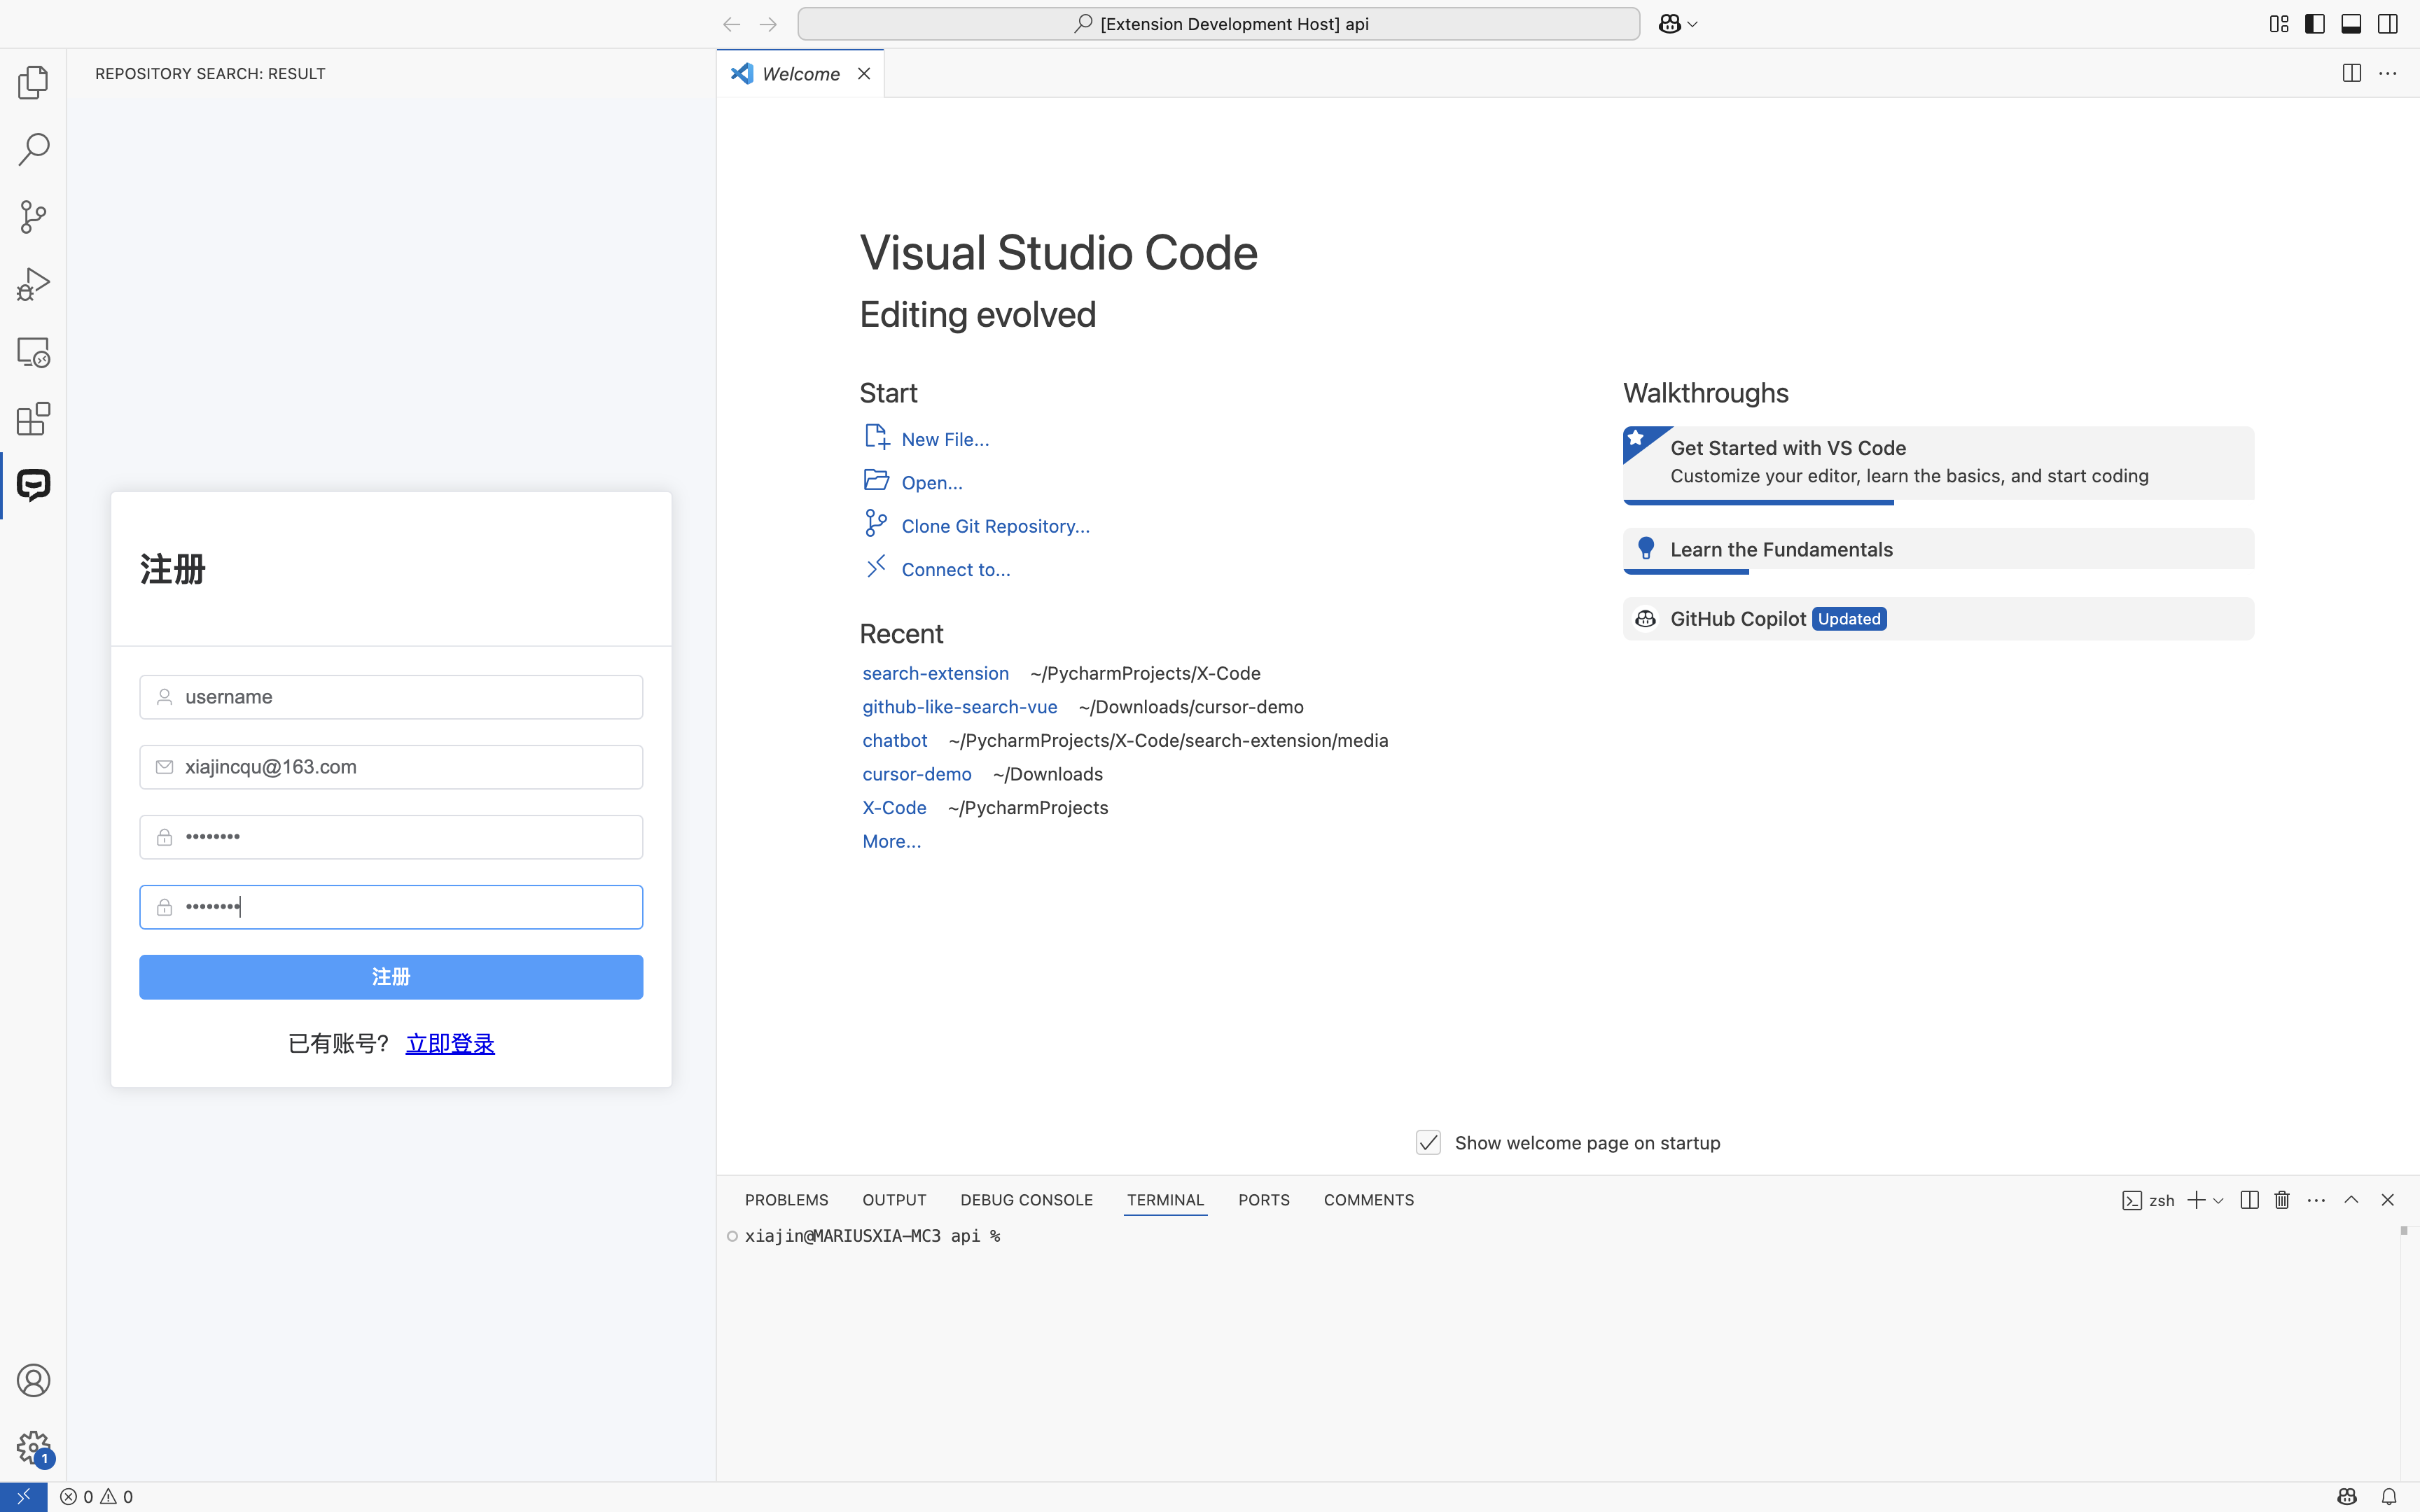
\includegraphics[width=0.95\textwidth]{register.png}}
	\caption{VS Code插件页面}
	\label{vscode}
\end{figure}
在登陆界面,如图\ref{logincheck}和图\ref{loginpage}所示,支持账号密码输入检测,防止空表单提交,提升系统安全性。用户信息在前端加密后传输至后端进行校验。
\begin{figure}[H]
	\center{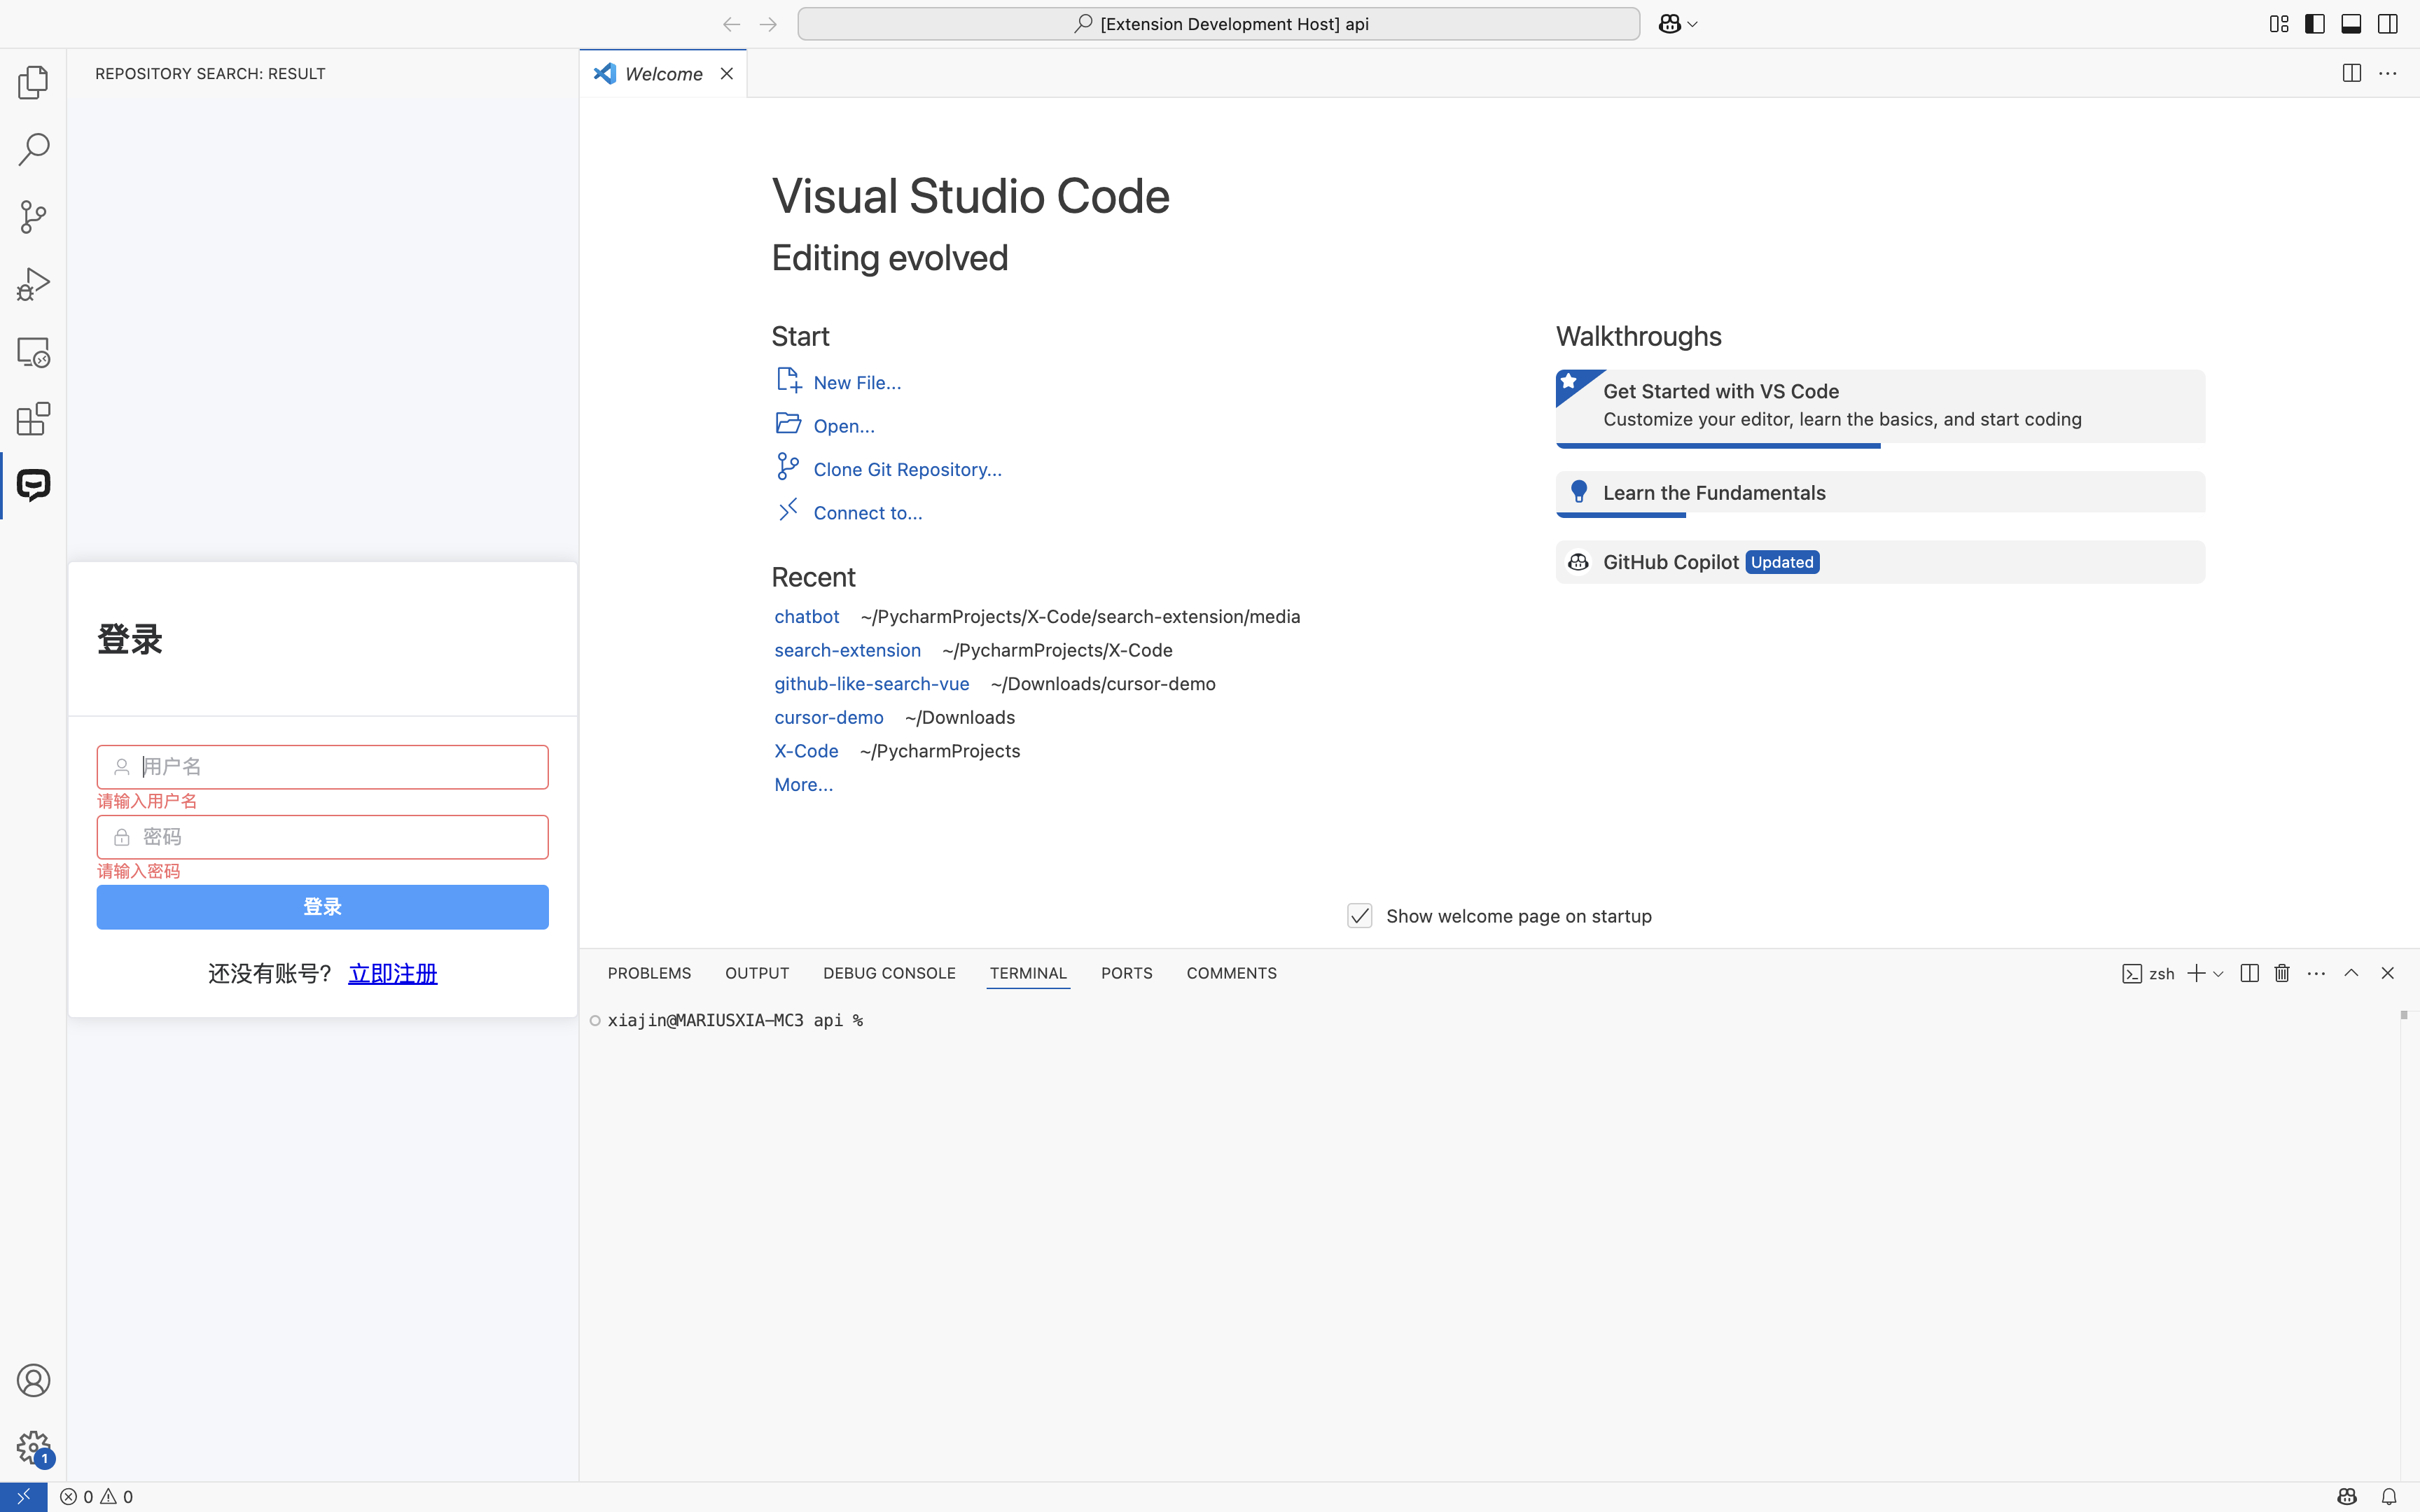
\includegraphics[width=0.95\textwidth]{login_check.png}}
	\caption{登录校验示例}
	\label{logincheck}
\end{figure}
\begin{figure}[H]
	\center{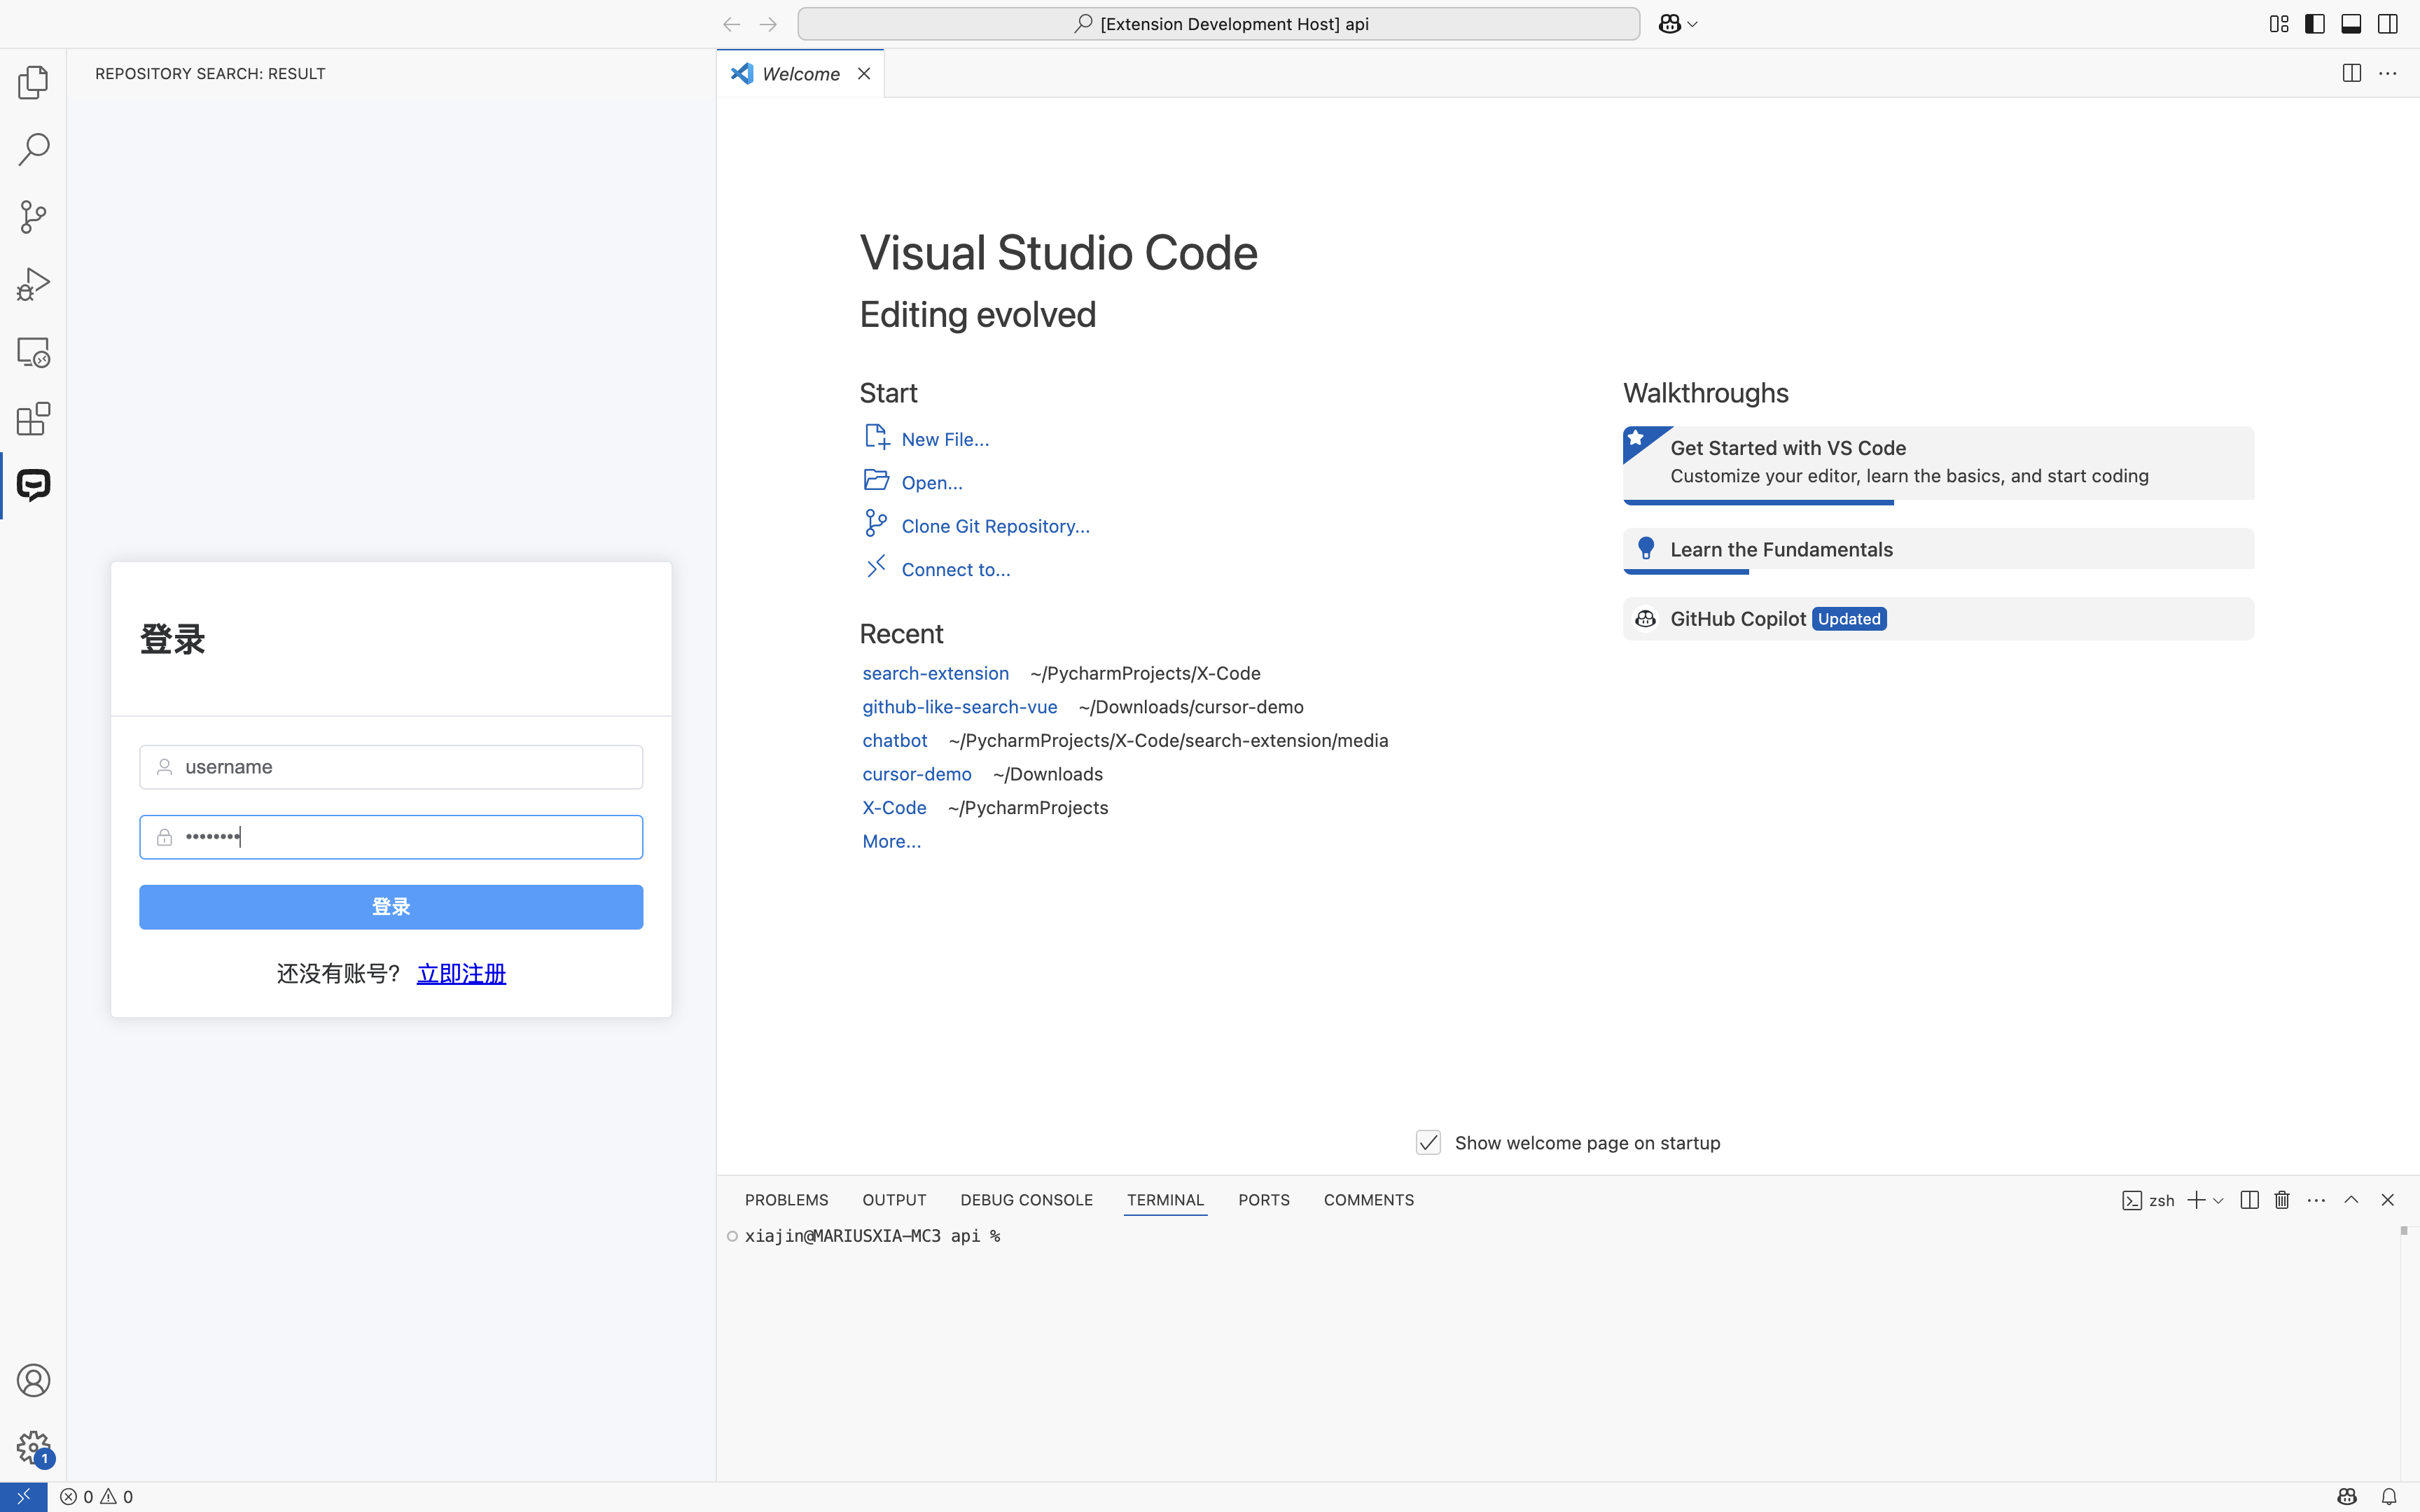
\includegraphics[width=0.95\textwidth]{login.png}}
	\caption{登录示例}
	\label{loginpage}
\end{figure}
注册页面同样具备输入检测功能,支持密码一致性校验,防止无效数据提交。如图\ref{registerpage}和图\ref{registercheckpage}所示。
\begin{figure}[H]
	\center{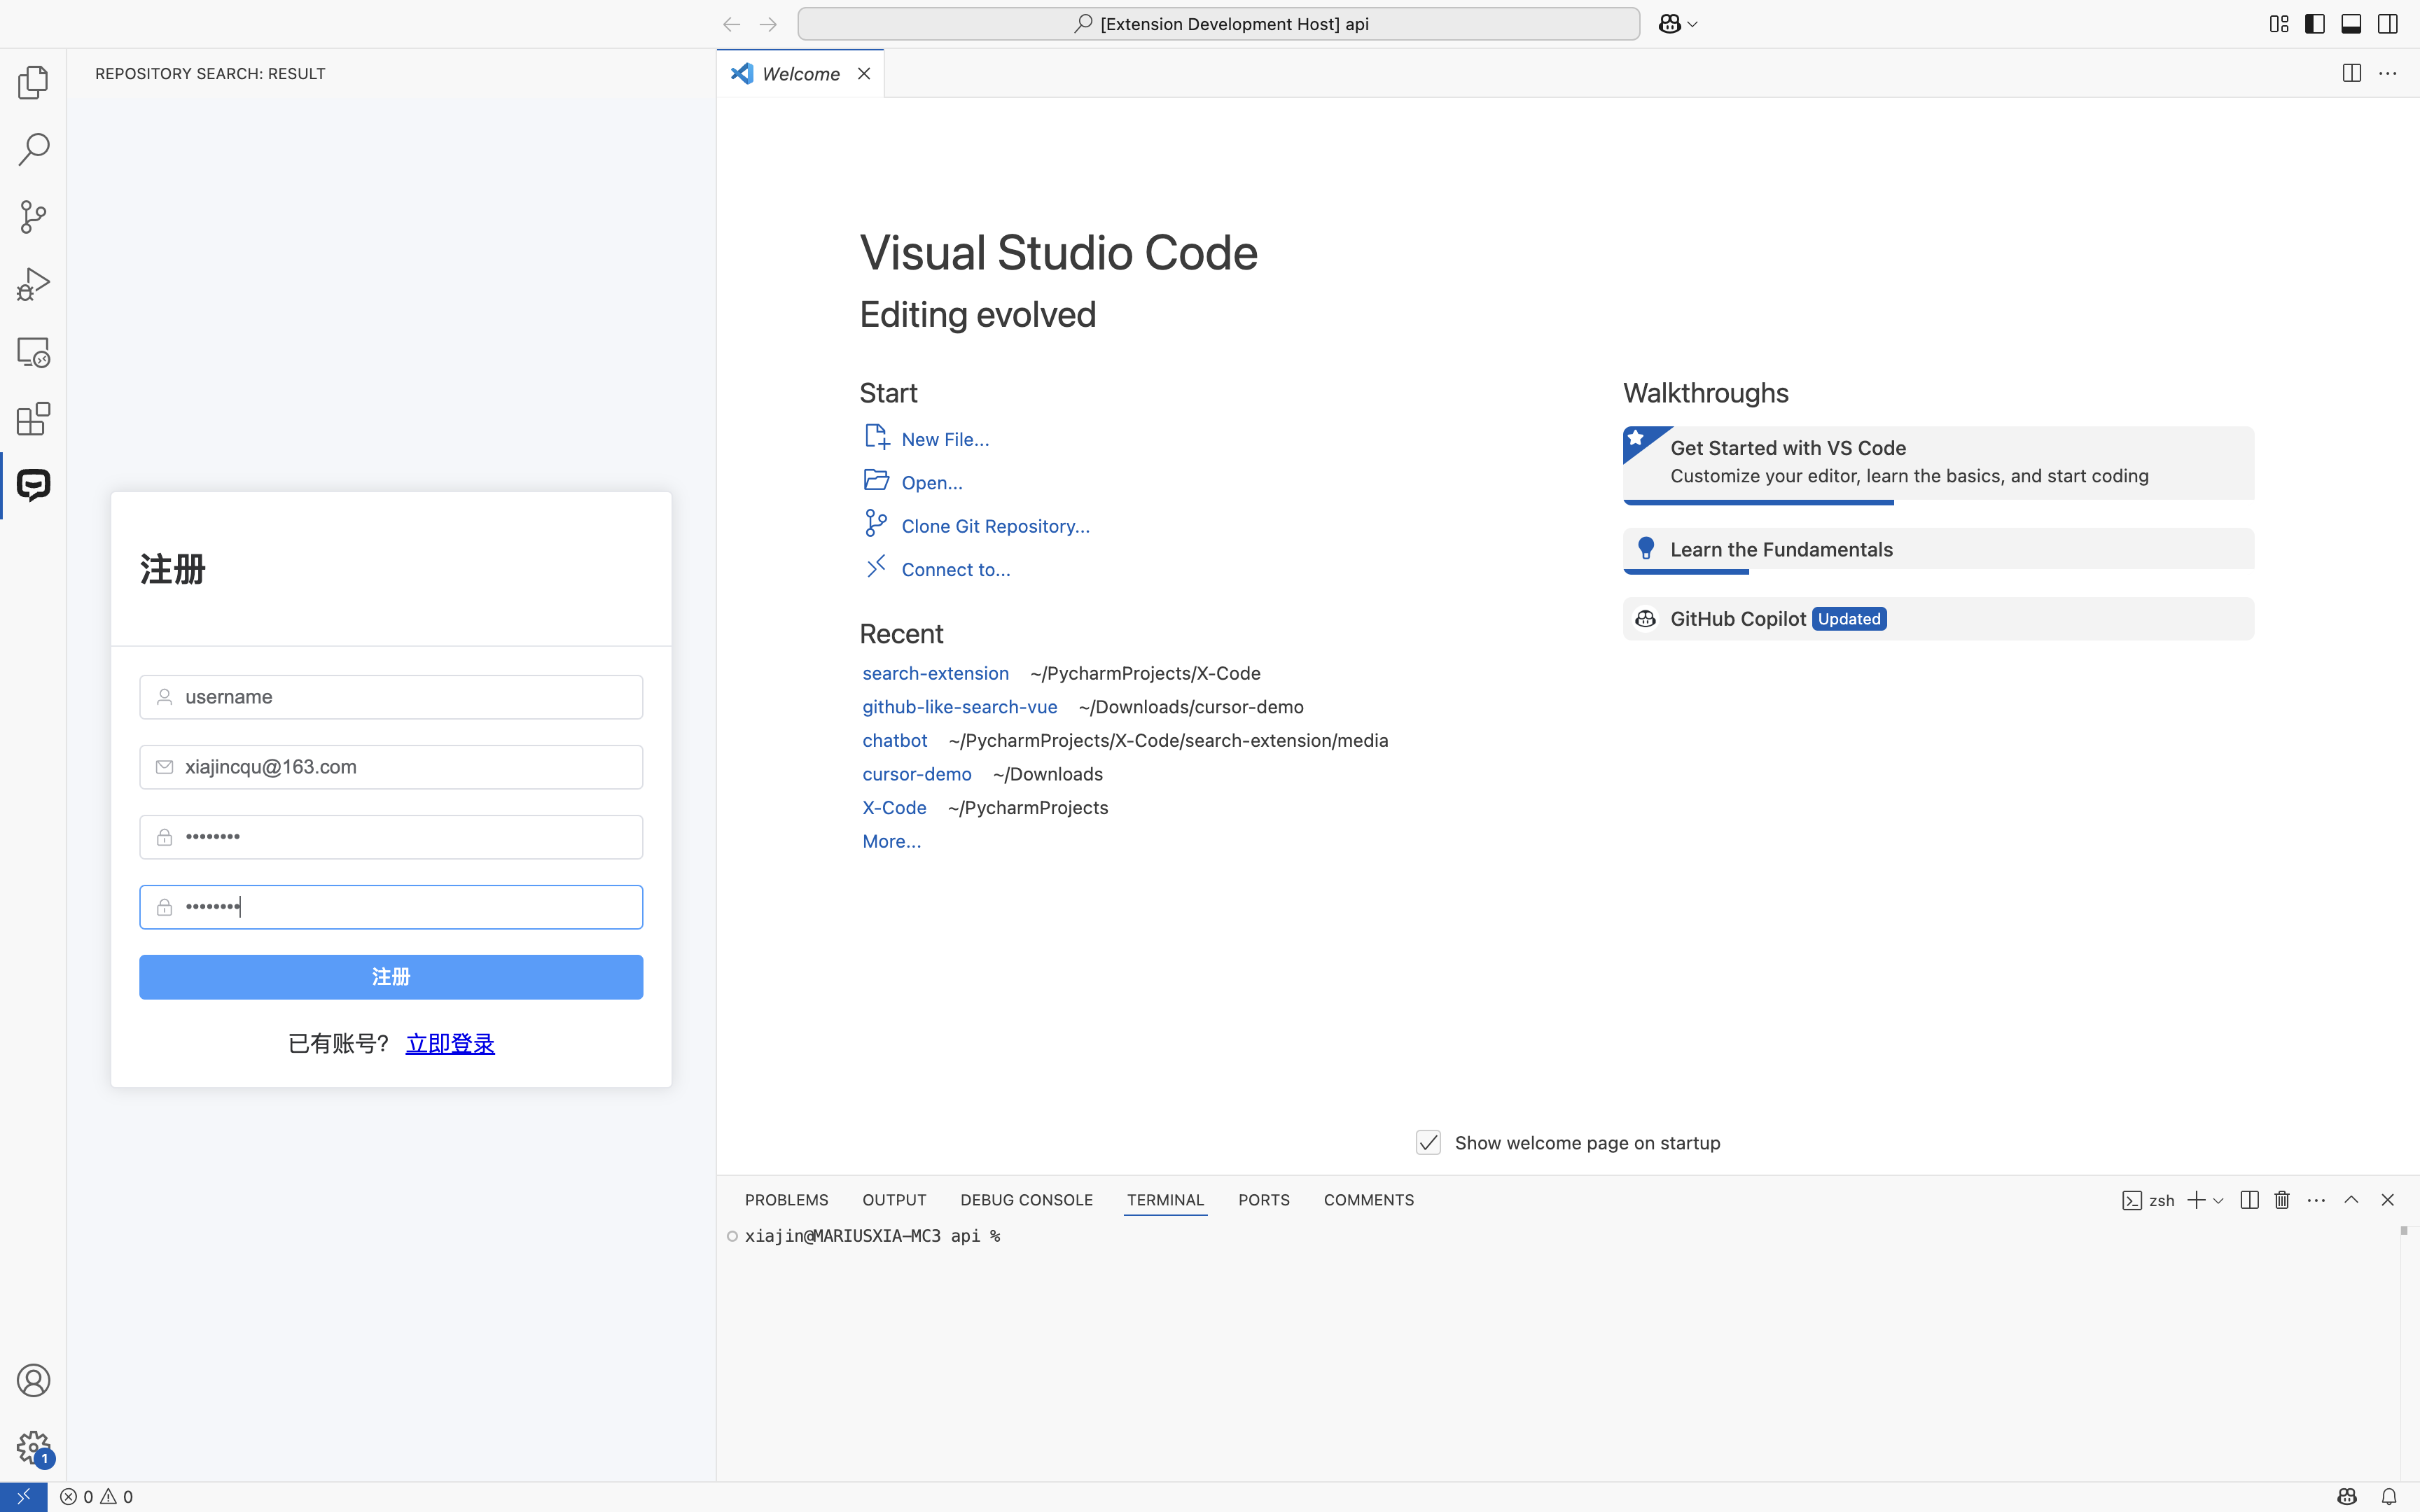
\includegraphics[width=0.95\textwidth]{register.png}}
	\caption{注册示例}
	\label{registerpage}
\end{figure}
\begin{figure}[H]
	\center{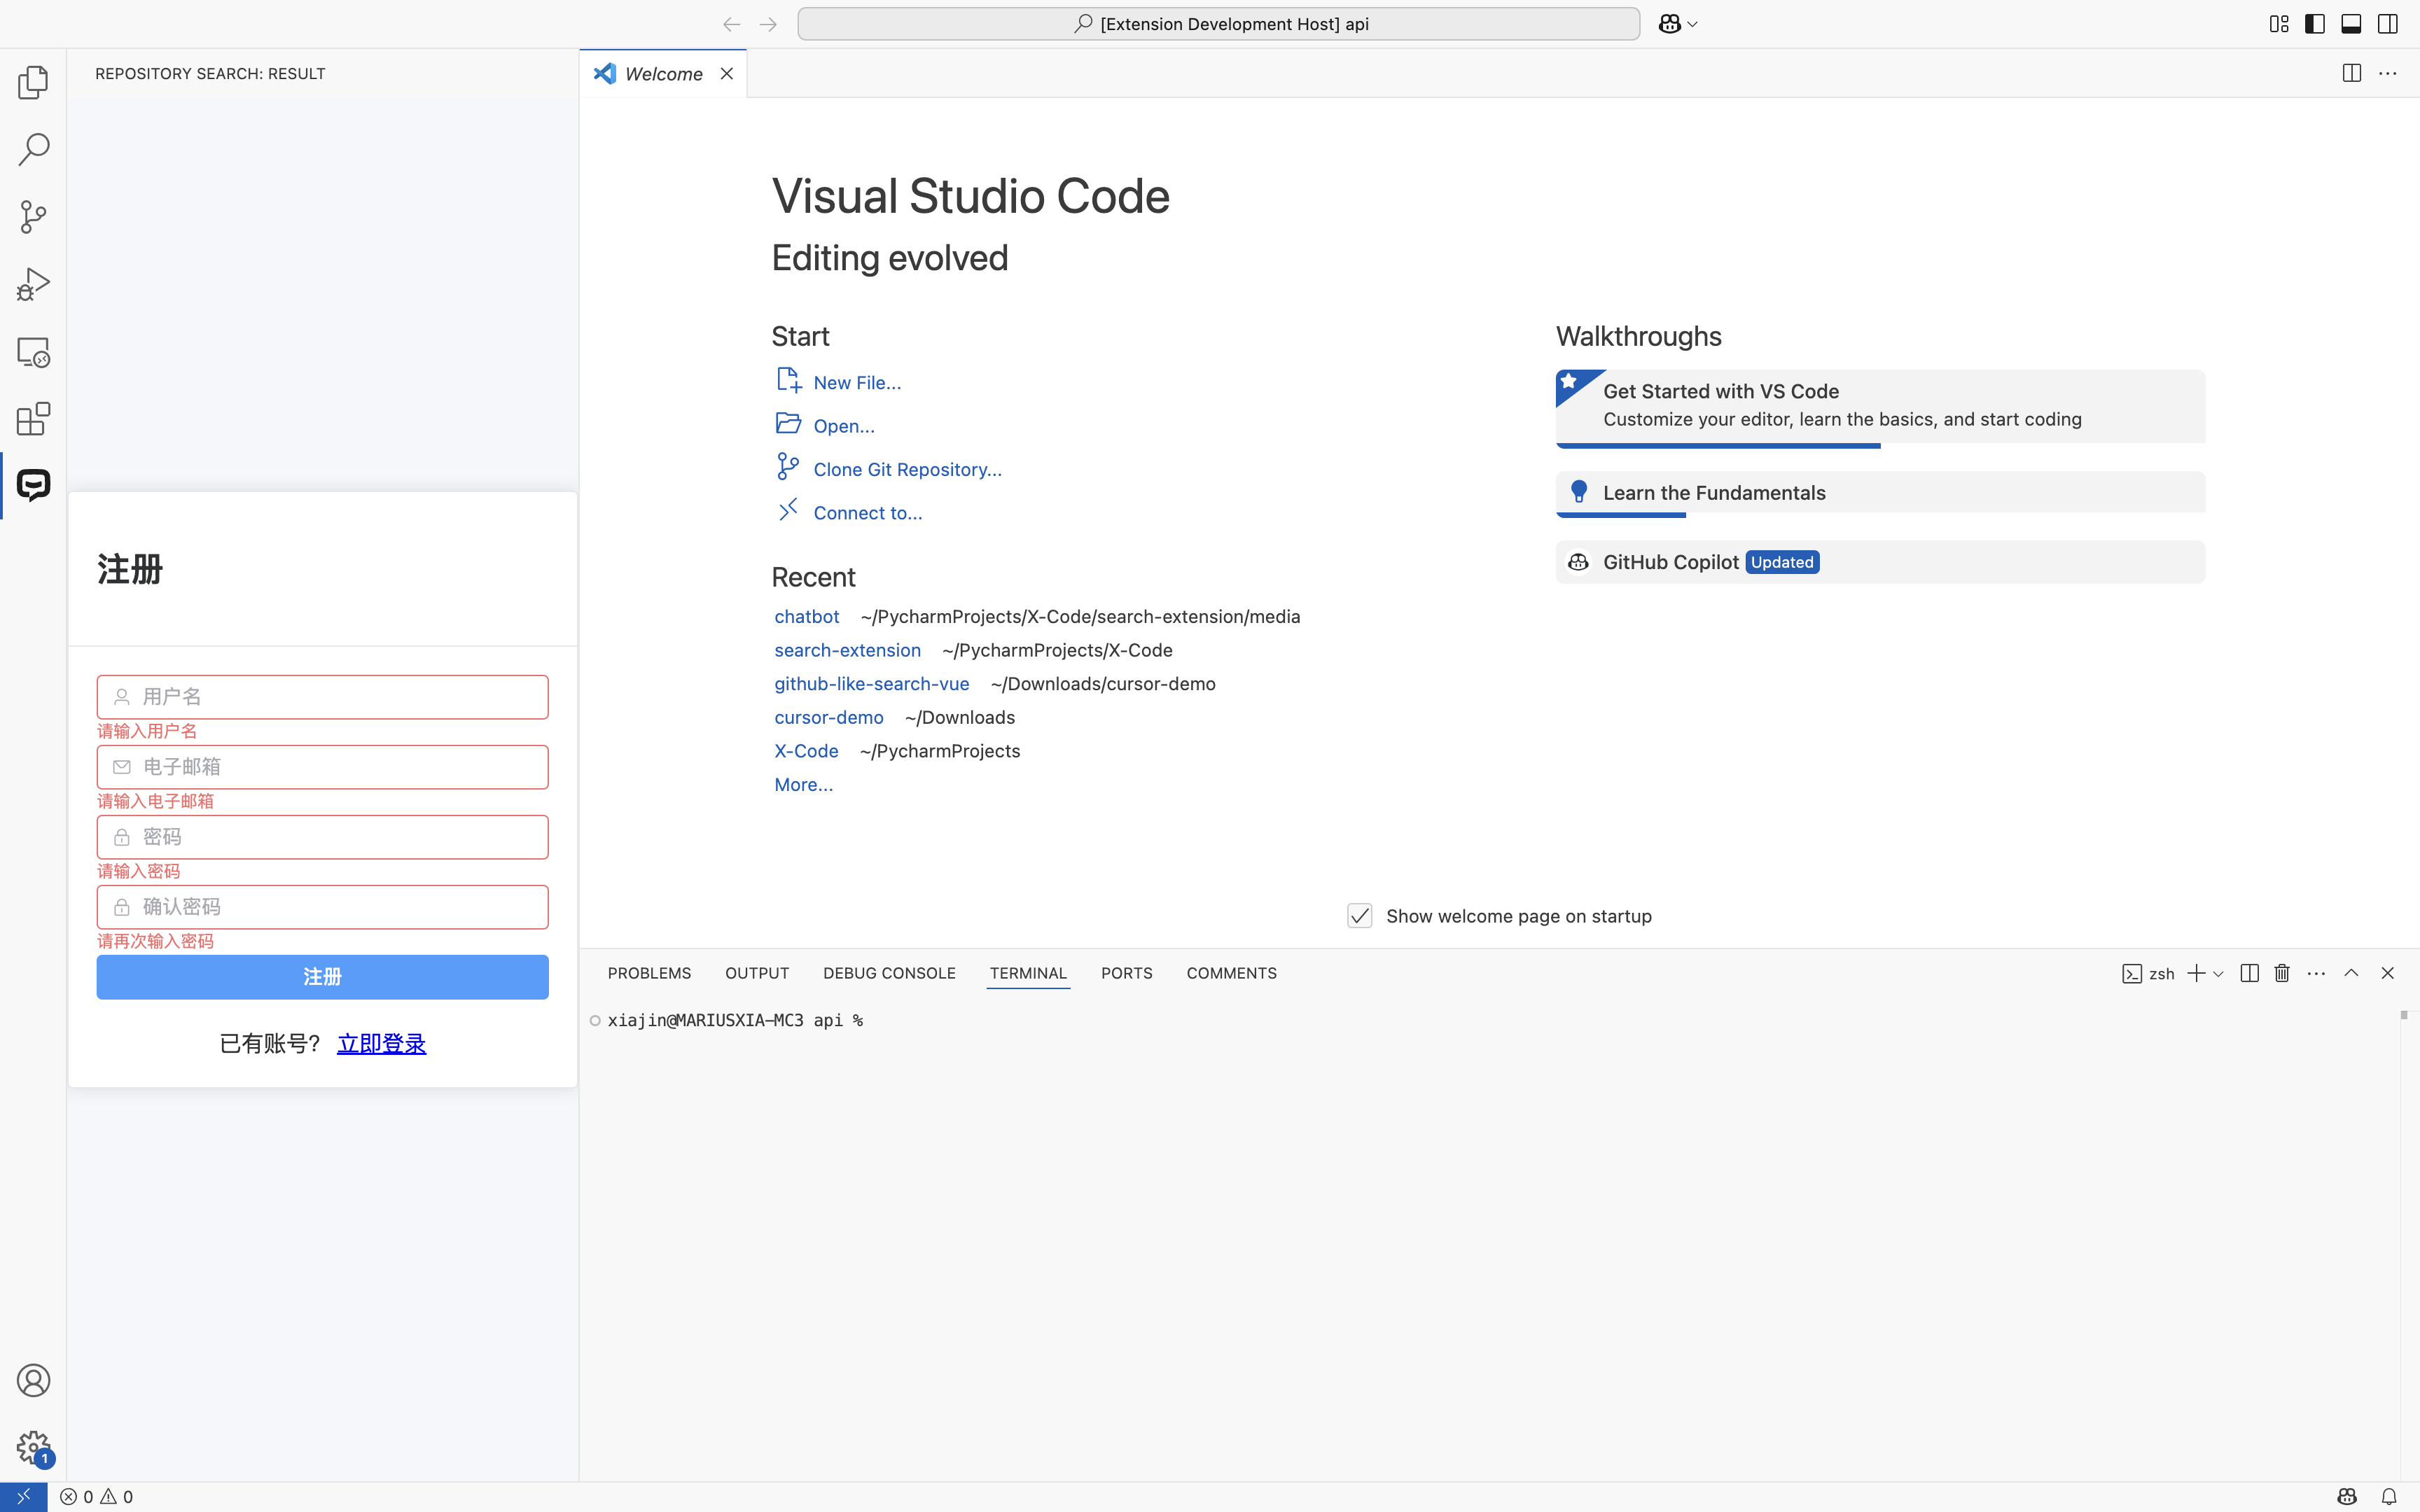
\includegraphics[width=0.95\textwidth]{register_check.png}}
	\caption{注册校验示例}
	\label{registercheckpage}
\end{figure}
系统的搜索页面设计简洁直观,用户可输入关键词进行代码检索。与传统搜索引擎不同,系统会对用户输入的查询词进行智能改写,并通过后端专业查询方法获取高质量结果。搜索结果以列表形式展示,支持项目选中高亮动画,提升交互体验。相关界面如图\ref{searchpage}和图\ref{select}所示。
\begin{figure}[H]
	\center{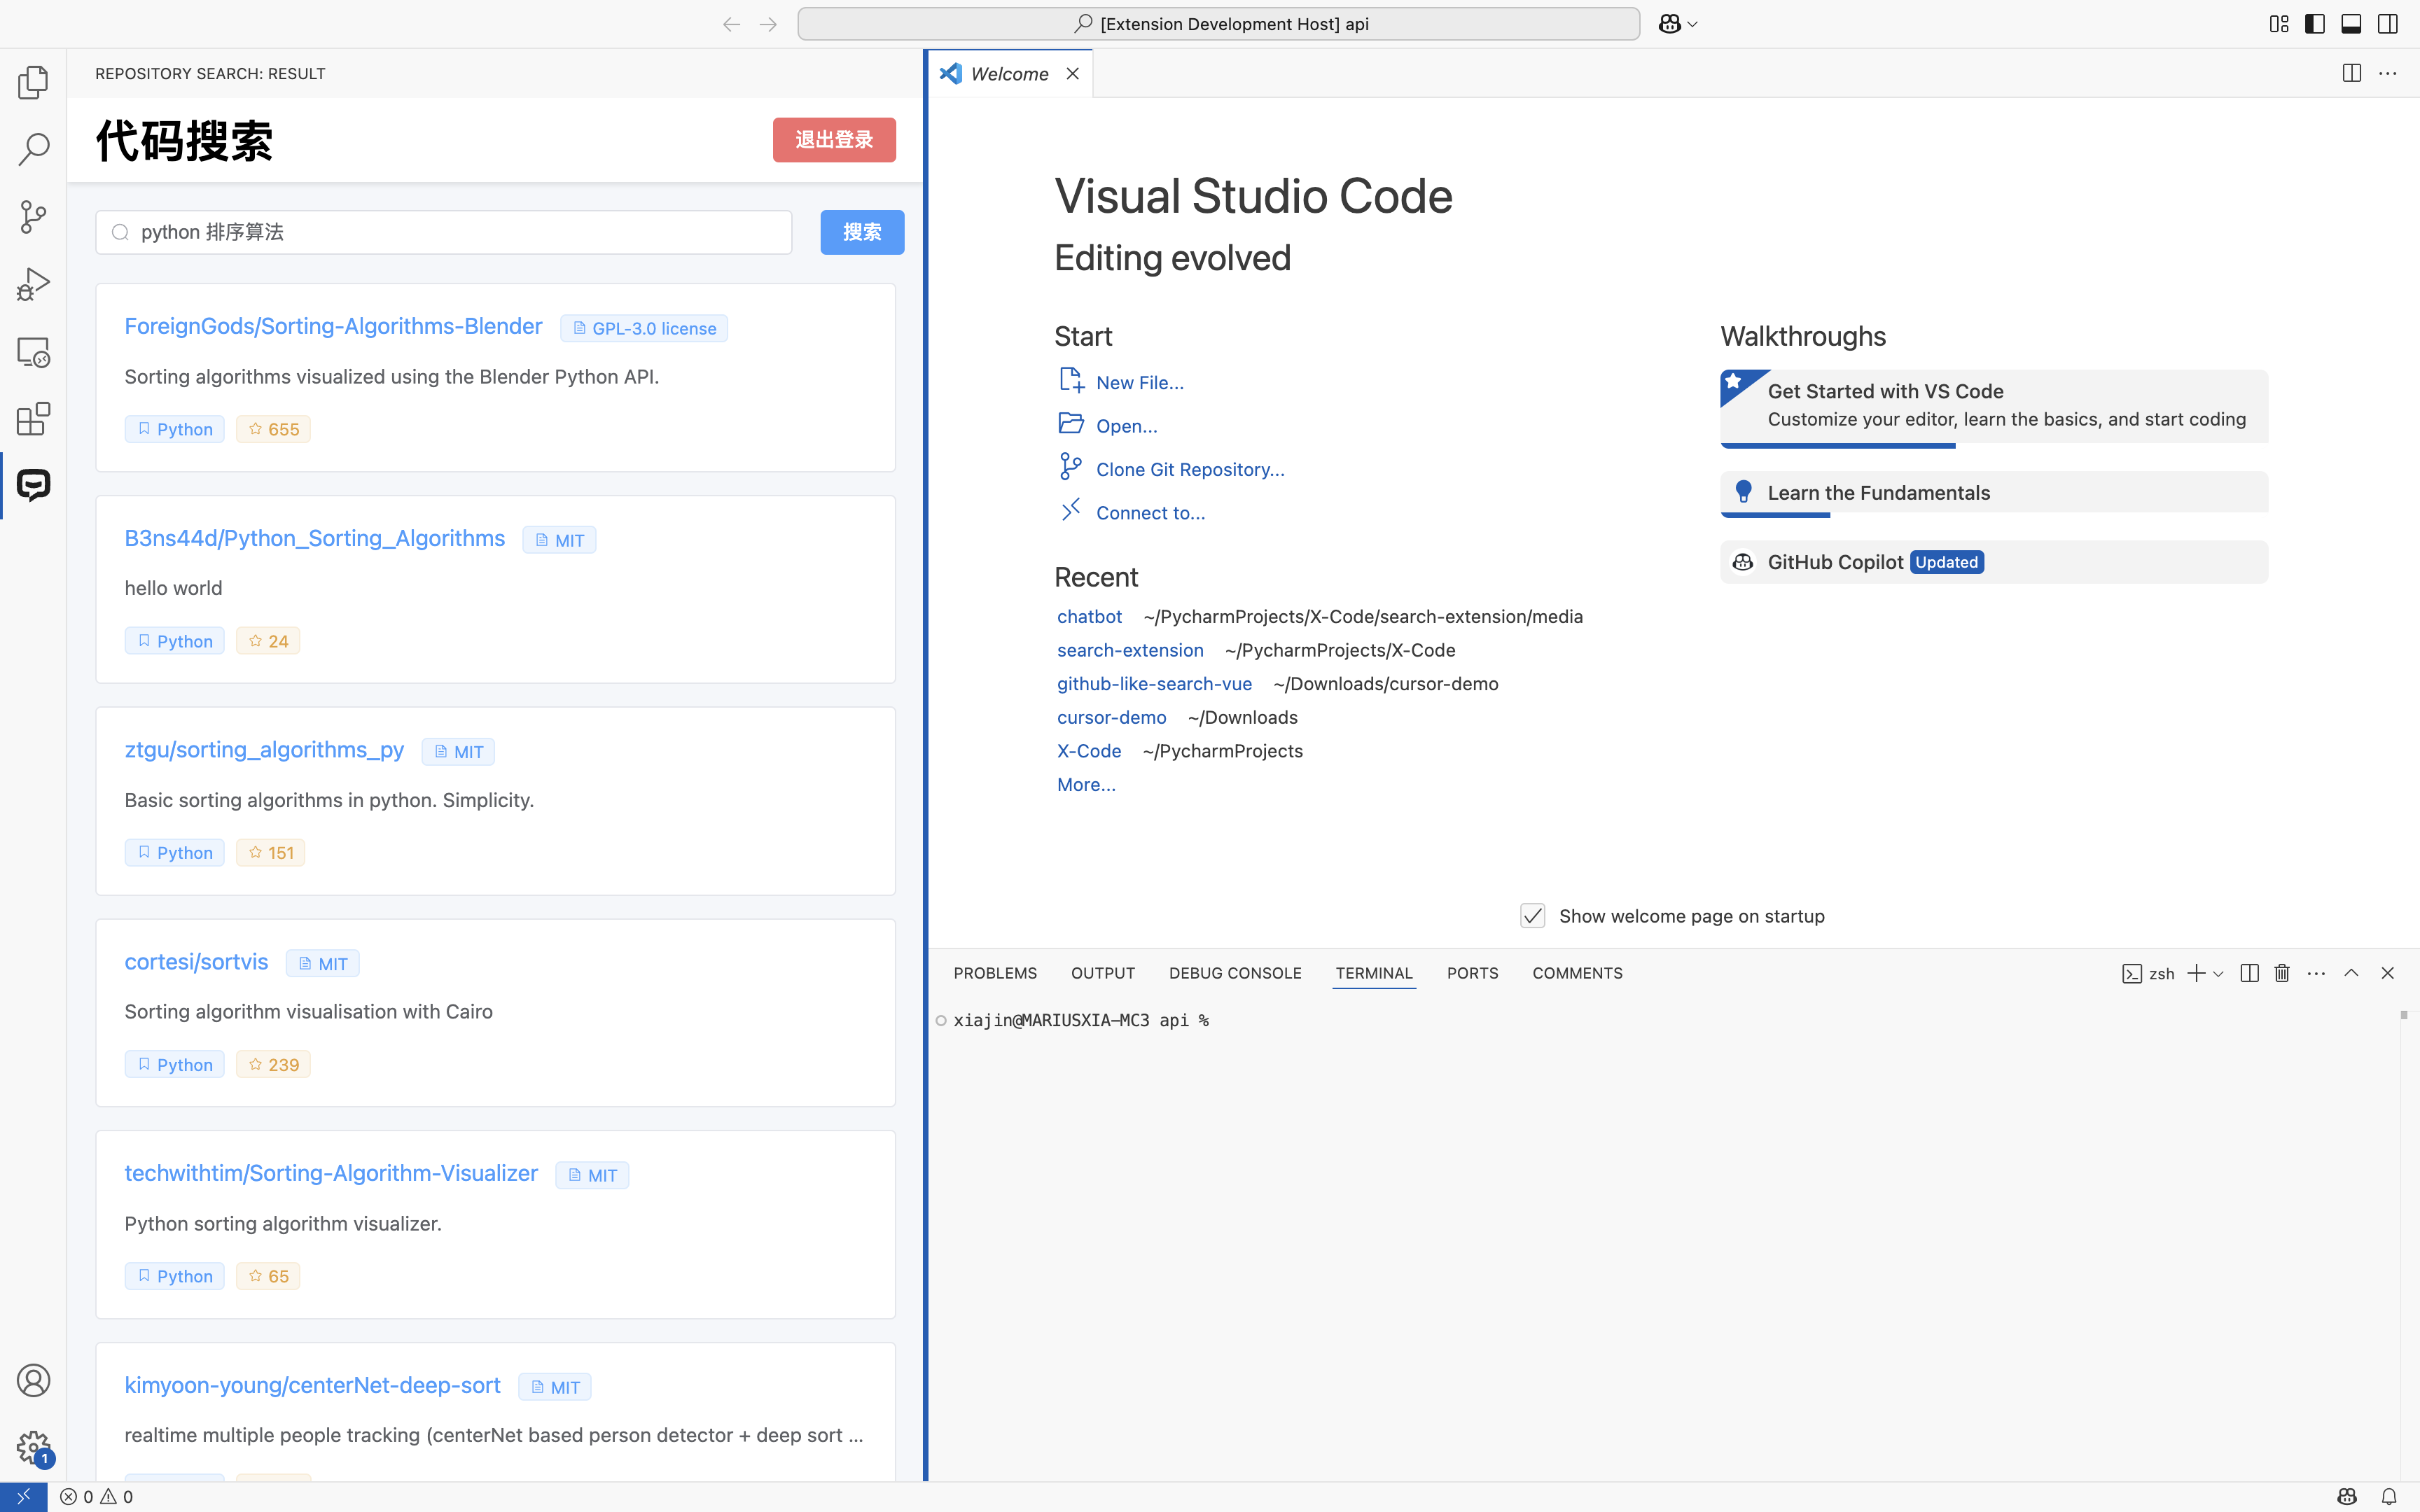
\includegraphics[width=0.95\textwidth]{search_page.png}}
	\caption{搜索页面示例}
	\label{searchpage}
\end{figure}
\begin{figure}[H]
	\center{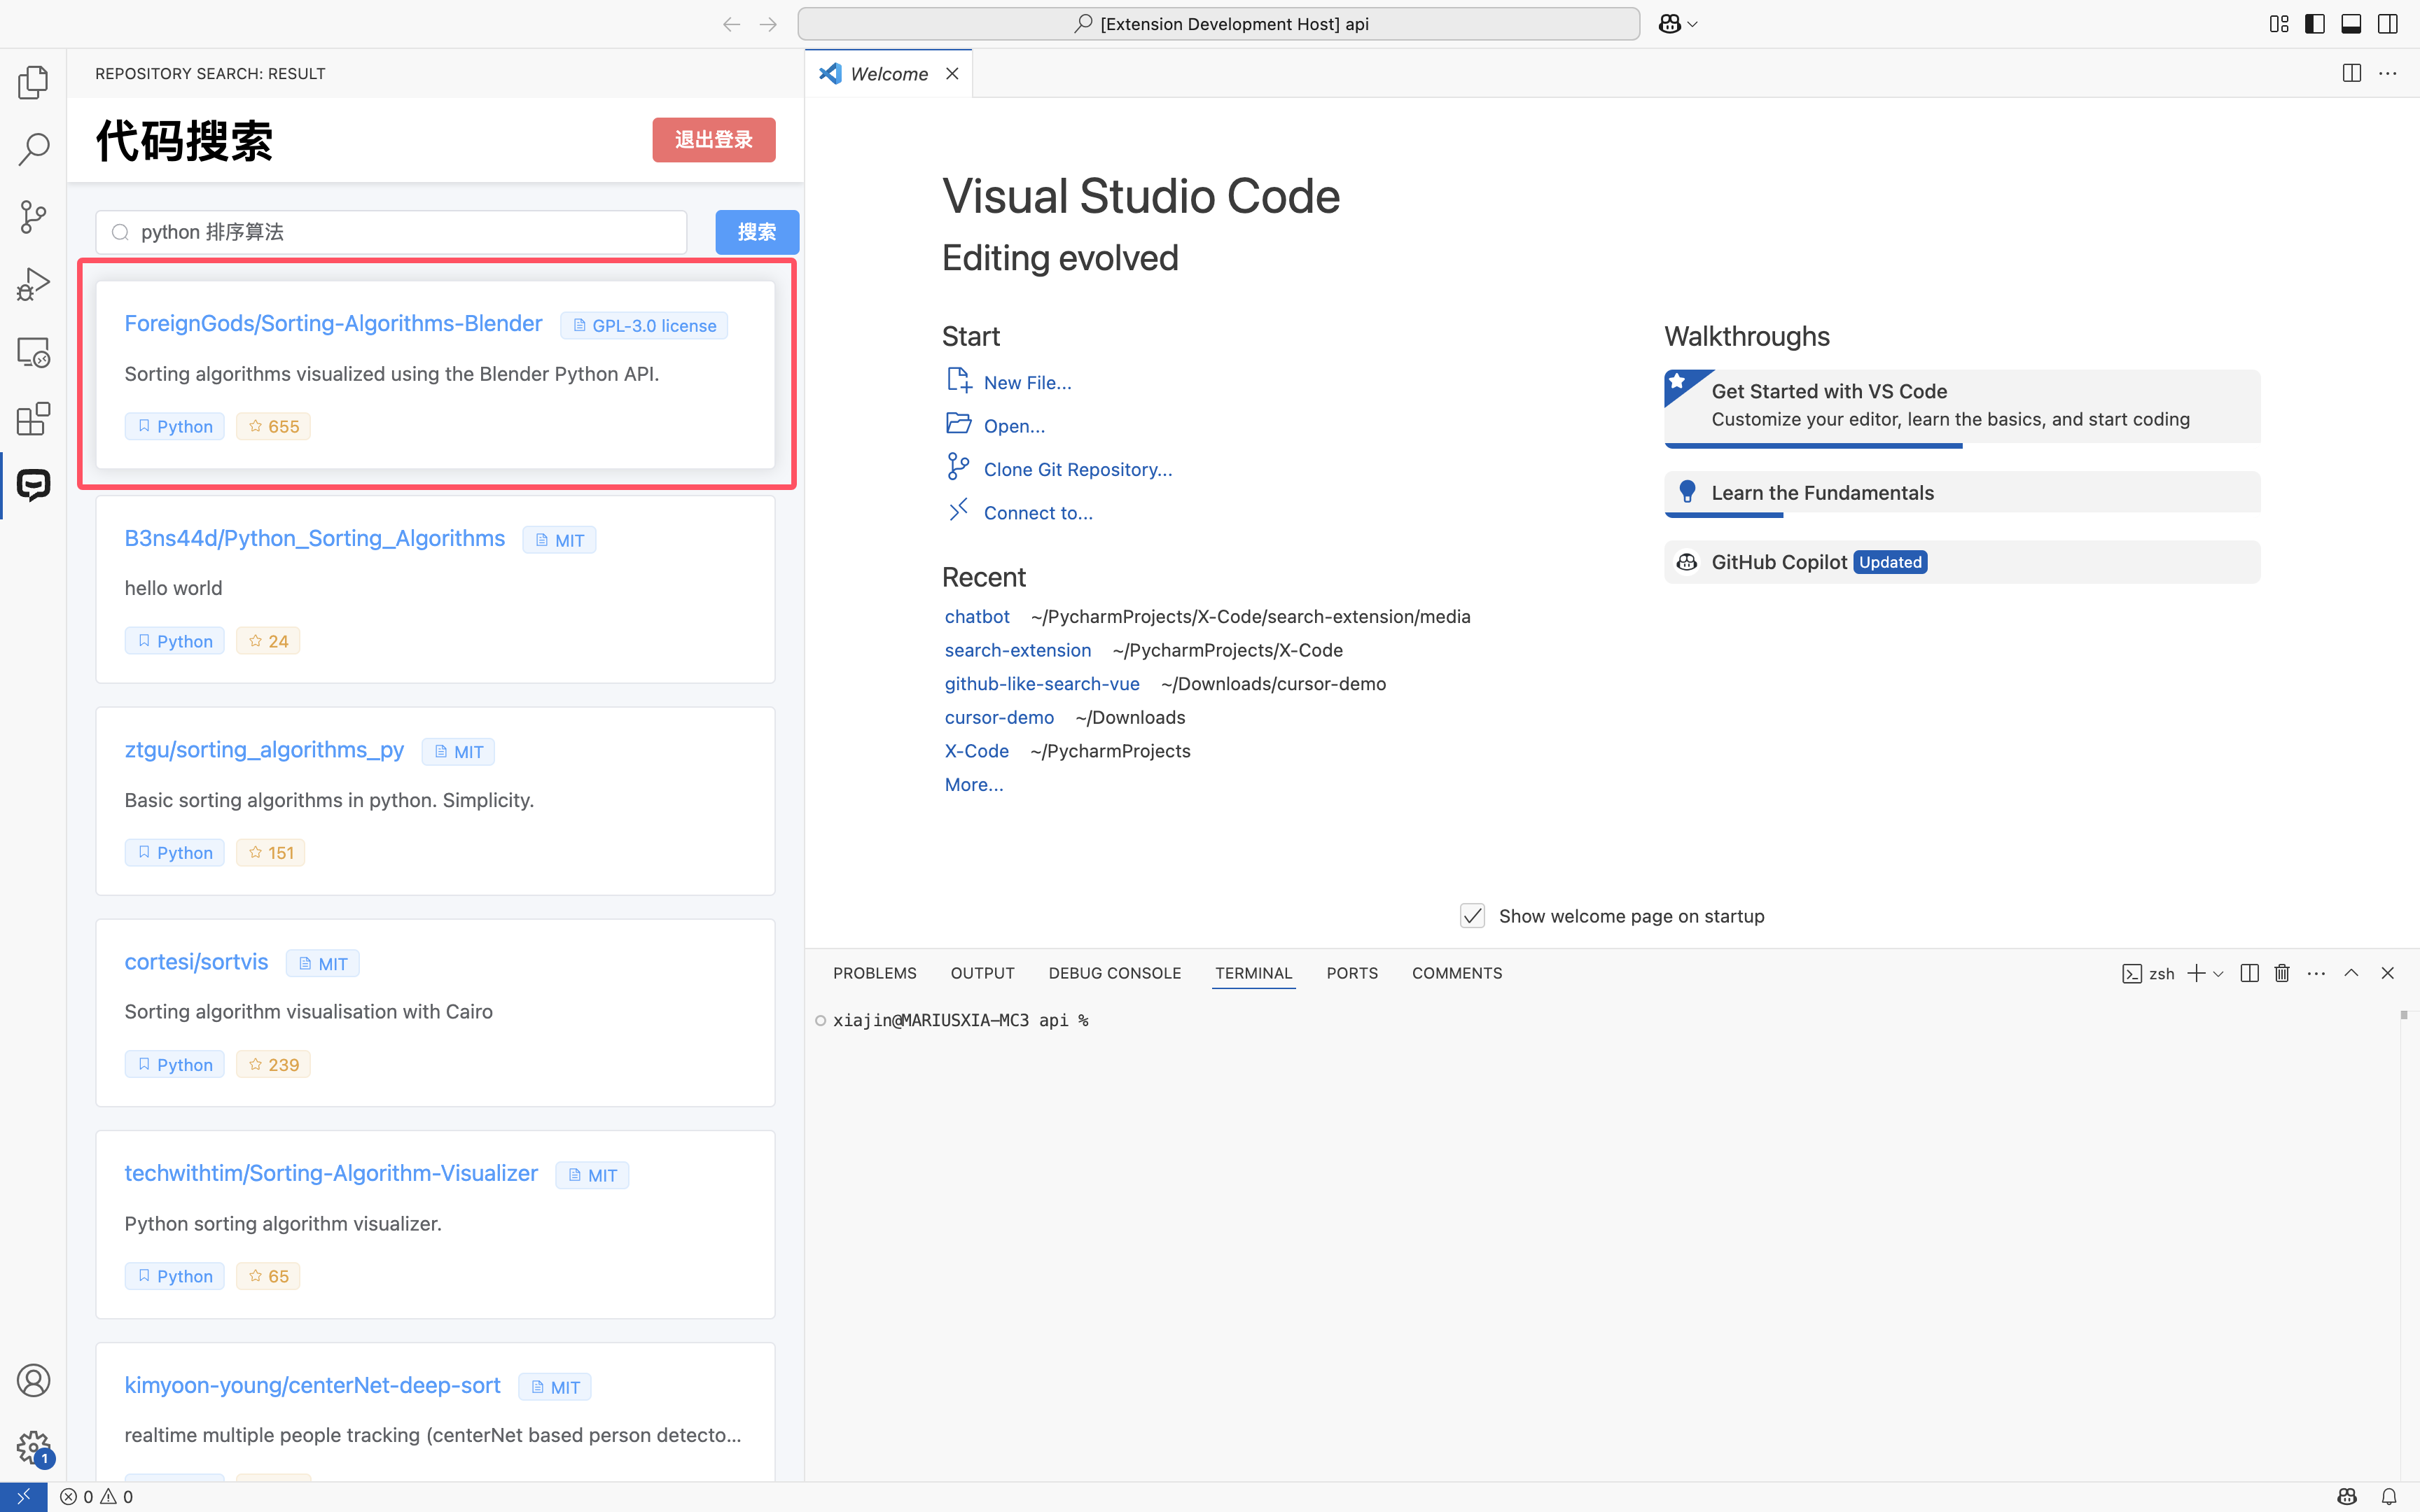
\includegraphics[width=0.95\textwidth]{search_select.png}}
	\caption{选中项目示例}
	\label{select}
\end{figure}
点击某一搜索结果后,用户可进入项目详情页面。该页面详细展示了项目名称、开源协议、项目描述、编程语言、星数、原始链接及文件列表,支持一键跳转至项目原网页,便于进一步浏览和分析。项目详情界面如图\ref{repodetailpage}所示。
\begin{figure}[H]
	\center{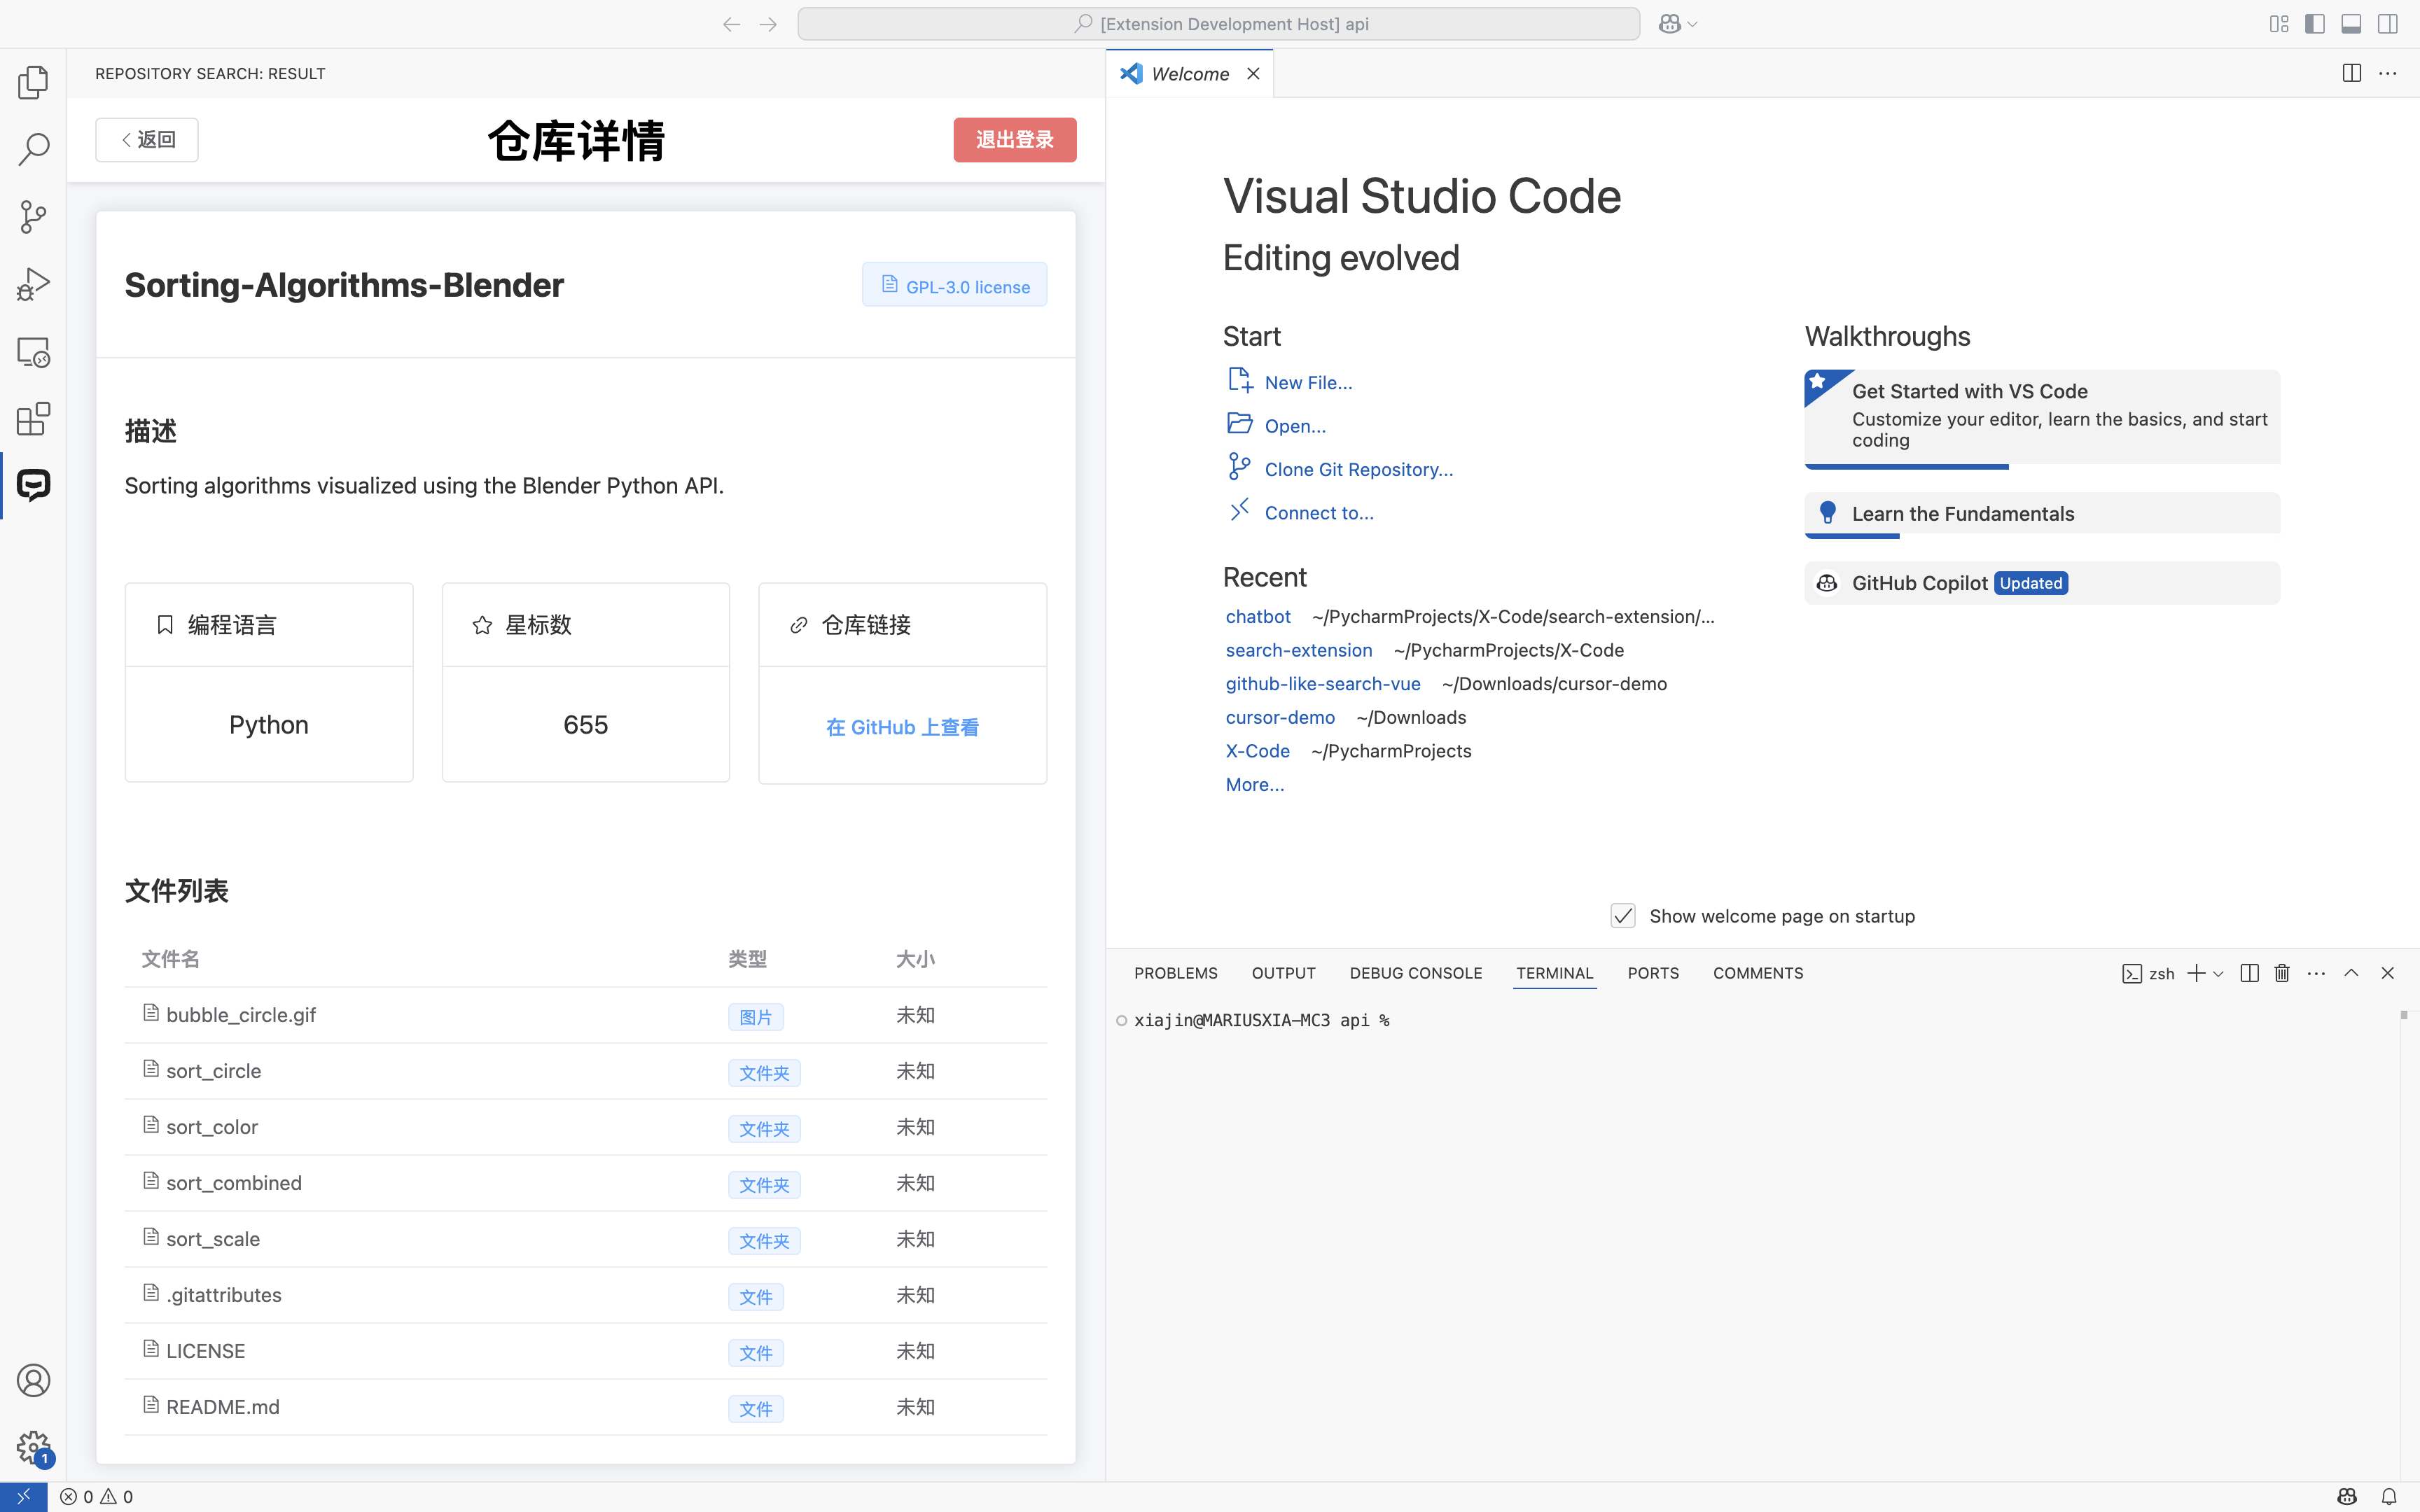
\includegraphics[width=0.95\textwidth]{repo_detail.png}}
	\caption{搜索详情示例}
	\label{repodetailpage}
\end{figure}
通过上述多端界面与分层架构的有机结合,系统实现了从用户注册、登录、代码检索到结果展示的完整闭环,极大提升了面向多编程语言的代码检索系统的易用性与用户体验。
\subsection{本章小结}

\section{总结与展望}

\newpage
\fancyhead[LH]{\zihao{-5}{\songti 重庆大学本科学生毕业论文(设计)}}
\fancyhead[RH]{\zihao{-5}{\songti 参考文献}}

\addcontentsline{toc}{section}{参考文献}
\renewcommand\refname{参考文献}

\zihao{5}

\begin{thebibliography}{1}
\setlength{\itemsep}{0pt}
\bibitem{1} 杨瑞林, 李力军. 新型低合金高强韧性耐磨钢的研究[J]. 钢铁. 1999(7): 41-45.
\bibitem{2} 于潇, 刘义, 柴跃廷, 等. 互联网药品可信交易环境中主体资质审核备案模式[J]. 清华大学学报(自然科学版), 2012, 52(11): 1518-1523.
\bibitem{3} Schinstock D.E., Cuttino J.F. Real time kinematic solutions of a non-contacting, three dimensional metrology frame[J]. Precision Engineering. 2000, 24(1): 70-76. 
\bibitem{4} 温诗铸. 摩擦学原理[M]. 北京: 清华大学出版社, 1990: 296-300.
\bibitem{5} 蒋有绪, 郭泉水, 马娟, 等. 中国森林群落分类及其群落学特征[M]. 北京: 科学出版社, 1998: 5-17.
\bibitem{6} 贾名字. 工程硕士论文撰写规范[D]. 重庆: 重庆大学, 2000: 177-178.
\bibitem{7} 张凯军. 轨道火车及高速轨道火车紧急安全制动辅助装置: 201220158825.2[P]. 2012-04-05.
\bibitem{8} 全国信息与文献标准化技术委员会. 文献著录: 第4部分 非书资料: GB/T 3792.4-2009[S]. 北京: 中国标准出版社, 2010: 3.
\end{thebibliography}
%(参考文献格式请参考GB/T 7714-2015《信息与文献 参考文献著录规则》)

\newpage
\fancyhead[LH]{\zihao{-5}{\songti 重庆大学本科学生毕业论文(设计)}}
\fancyhead[RH]{\zihao{-5}{\songti 附录A:XX公式的推导}}

\addcontentsline{toc}{section}{附录A:XX公式的推导}
\section*{致\quad 谢}
\zihao{-4}
致谢主要感谢导师和对论文工作有直接贡献和帮助的人士和单位。致谢言语应谦虚诚恳,实事求是。

\newpage
\thispagestyle{empty}

\addcontentsline{toc}{section}{原创性声明和使用授权书}
\begin{center}
\heiti \zihao{3}
原创性声明
\end{center}

\songti\zihao{-4}
郑重声明:所呈交的论文(设计)\underline{《  \hspace{6em}》},是本人在导师的指导下,独立进行研究取得的成果。除论文(设计)中已经标注引用的内容外,本论文(设计)不包含其他人或集体已经发表或撰写过的作品成果。对本文的研究做出贡献的个人和集体,均已在文中以明确方式标明。本人完全意识到本声明的法律后果,并承诺因本声明而产生的法律结果由本人承担。

~\\
\begin{flushleft}
\begin{tabular}{l}
\songti\zihao{-4}
论文(设计)作者签名: \underline{\hspace{6em}}\\
\songti\zihao{-4}
日期:\underline{\hspace{6em}}
\end{tabular}
\end{flushleft}

~\\
\begin{center}
\heiti \zihao{3}
使用授权书
\end{center}

\songti\zihao{-4}
本论文(设计)作者完全了解学校有关保留、使用论文(设计)的规定,同意学校保留并向国家有关部门或机构送交论文(设计)复印件和电子版,允许论文(设计)被查阅和借阅。本人授权重庆大学将本论文(设计)的全部或部分内容编入有关数据库进行检索,可以采用影印、缩印或扫描等复制方式保存和汇编本论文(设计)。

~\\
\songti\zihao{-4}
本论文(设计)属于:\par
保\quad 密 $\Box$  \quad 在\underline{\qquad}年解密后适用本授权书\par
不保密 $\Box$

~\\
~\\
\begin{flushleft}
\songti\zihao{-4}
\begin{tabular}{l l}
论文(设计)作者签名:\underline{\hspace{6em}} \hspace{300mm}&指导教师签名:\underline{\hspace{6em}} \\
日期:\underline{\hspace{6em}} &日期:\underline{\hspace{6em}}\\
\end{tabular}
\end{flushleft}

\end{document} 